% For printing in a4
%\documentclass[a4,10pt,twoside,openright,italian,english]{book}% twoside!
\RequirePackage{silence}
\WarningFilter{scrreprt}{Usage of package `titlesec'}
\WarningFilter{scrreprt}{Activating an ugly workaround}
\WarningFilter{titlesec}{Non standard sectioning command detected}
% For printing with the A5 format
%\documentclass[10pt,twoside,openright,english]{book}% twoside!
\documentclass[ 
%draft,
                fontsize=9pt,
                oneside,
                twoside,
                openright,
                titlepage,
                dottedtoc,
                a5paper,
                fleqn,%
                headinclude,
                footinclude=true,
                BCOR=10mm,%
                DIV=12,
                numbers=noenddot,
                cleardoublepage=empty
                ]{scrbook}
\input{thesis_init2.tex}



% \includeonly{chapters/ack}
% \includeonly{chapters/introduction}
% \includeonly{chapters/chapter1}
% \includeonly{chapters/chapter3}
% \includeonly{chapters/chapter4}
% \includeonly{chapters/chapter5}
% \includeonly{chapters/chapter6}
% \includeonly{chapters/chapter7}
\includeonly{chapters/chapter8}
% \includeonly{chapters/appendix1}
% \includeonly{chapters/appendix2}


%\includeonly{chapters/introduction}

%%%%%%%%%%%%%%%%%%%%%%%%%%%%%%%%%%%%%%
% Let's Start The Real Document
%%%%%%%%%%%%%%%%%%%%%%%%%%%%%%%%%%%%%%
\begin{document}
\selectlanguage{english}

\cleardoublepage
\maketitle

\pagestyle{empty}

\cleardoublepage
\newpage
\newpage

%%%%%%%%%%%%%%%%%%%%%%%%%%%%%%%%%%%%%%
% Acknowledgement
%%%%%%%%%%%%%%%%%%%%%%%%%%%%%%%%%%%%%%
 \chapter*{Acknowledgements}
 
 This work has been supported by research grants within the following research projects:
\begin{itemize}
 \item[] SINOPIAE project, from the Italian Ministry of University and Research and Regione Lombardia
 \item[] MEP: Maps for Easy Paths project funded by Politecnico di Milano under the POLISOCIAL program
 \item[] I.DRIVE Inter-department Laboratory Grant from Politecnico di Milano
\end{itemize}
We also thank NVIDIA who kindly supported this work through the Hardware Grant Program.


\bigskip 



Aside from the institutional acknowledgements, I also want to thank all the people who supported me in these four years of PhD. 
I am especially grateful to my Sara, that will be soon my wife; she has been close to me for all this time and she went through my deadline madnesses and my overnight clikkety clikings.
I thanks my mother,  Gianni, and all my family that, for better or for worse, they had took a huge role in who I am.
I thank my old and new friends and my PhD companion who shared with me all the joy and sorrow of these four years, in particular, Francesco.  
I thank of course my advisor Matteo who supported me financially but especially who drove me through the crowded jungle of academics
Finally, I want to acknowledge Prof. Marc Pollefeys who kindly hosted me in his laboratory and Amaël Delaunoy who gave me useful advices and in-sights about Multi-View Stereo.



\cleardoublepage
\newpage

%\pagestyle{fancy}
% change numbering into Roman numbers for the introductory part
\setcounter{page}{1}
\pagenumbering{Roman}
\pagenumbering{roman}
\pagestyle{plain}

%%%%%%%%%%%%%%%%%%%%%%%%%%%%%%%%%%%%%%
% Abstract
%%%%%%%%%%%%%%%%%%%%%%%%%%%%%%%%%%%%%%
\chapter*{Abstract}
\vspace{-5pt}

 

In the last decade, the growing interest about autonomous driving brought many computer vision and robotics researchers to focus on the  vehicles understanding of the surrounding environment through a map of it.
A map is needed to plan a path to reach a specific destination, or to estimate the current position by comparing the current perception of the environment against a reference.
In robotics, a suitable mapping, or reconstruction, algorithm needs  to be scalable, incremental and to provide a dense map. 
Scalability is needed especially in large-scale environments; an incremental algorithm allows map update as new data are acquired; density enables a consistent and coherent navigability.
Researchers, in computer vision, focused their reconstruction algorithms on accurate and dense results, disregarding any incremental processing, and only few works shows large-scale capabilities.  
Instead, in robotics the focus is mainly on incremental algorithms but the output maps are usually point clouds; only a very limited amount of works estimate dense and continuous surfaces, but they are limited to small scale scenes.
As the main contribution of this thesis, we propose a novel incremental, automatic and scalable reconstruction  pipeline to estimates continuous dense manifold meshes; we especially focused on keeping the manifold property valid, to enable a coherent mesh refinement based on image appearance.  
Our contribution first improves the accuracy of the state-of-the-art incremental reconstruction algorithm both in case of video sequences of urban landscape, and in case of unordered set of images.
Then, to embed and refine automatically and incrementally new part of the scene in a reference  model, we proposed a novel mesh merging algorithm that preserves the manifold property.
Finally, we extended our work to jointly deal with laser range finders and images, exploiting the accuracy of the laser range measurement and the appearance provided by the images.
We tested our proposals against publicly available KITTI, Middlebury and EPFL datasets, which provide different scenarios in order to stress the flexibility of our approach.




%%%%%%%%%%%%%%%%%%%%%%%%%%%%%%%%%%%%%%
% TOC
%%%%%%%%%%%%%%%%%%%%%%%%%%%%%%%%%%%%%%
\dominitoc% Initialization
\tableofcontents
\cleardoublepage
\newpage

% Now lets go back to normal numbering
\setcounter{page}{1}
\pagenumbering{arabic}

\cleardoublepage
\newpage

\chapter{Introduction}
\label{sec:intro}
We are in the era of autonomous driving: vehicles endowed with a wide variety of sensors, are becoming  capable to navigate more and more challenging environments.
As the humans use mostly vision among their senses to perceive and act, the vehicles could heavily rely on images perceived by the cameras to interact with the surrounding.
Indeed, many advancements towards the autonomous driving have been achieved thanks to the joint efforts of Computer Vision and Robotics communities.
Computer Vision aims at extracting meaningful information from images such as the class the subject belongs to, the action happening in the scene or the 3D model of the environment, while Robotics aims at designing robots, or autonomous machines, and at deploying them in the real world.

One of the key aspect needed to navigate is the knowledge of the map of the environment. 
In Robotics and Computer Vision, visual mapping and 3D reconstruction, represent two very active research fields.
Early works of Robotics focuses especially in the creation of the map while the camera is navigating through an environment, leading to the so called Simultaneous Localization and Mapping (SLAM) algorithms.  Computer Vision researchers not only tried to recover the joint motion of the camera together with the structure with the Structure from Motion (SfM) algorithms, which are close to SLAM, but they also focused on the reconstruction of a detailed and accurate dense 3D model of the environment.





have been proposed to navigate through an environment without the map, in real world scenario we need to decouple these aspects in order to achieve both robustness and speed.
If a map of the environment is known, the robot is able to localize itself and navigate through them following a path defined by the user.
 it aims at building a 3D model of environment assuming that the pose of the camera is known from external calibration, for instance from explicit measurements, from telemetry or self-calibration algorithms.
While Robotics focuses on the real-time capabilities of the algorithm and 

multi view

robotics mostly slam


dicotomia robotics e computer vision

\section{Motivation}
In the last decade, many mapping approaches have been proposed; they differ from various aspects, e.g., initialization, optimization procedure, 3D model representation.

The scene can be represented by different geometric entities: point, 3D patches, volumes or surfaces.
Points are adopted when the computational time is the limited resource, for instance, in Robotics when Simultaneous Localization and Mapping, and algorithm relying on 3D patches show impressive results on highly textured scenes. 
These representations cannot be adopted for robot navigation, since they are sparse, therefore not a continuous navigable surface.
%All the feature-based and semi-dense SLAM approaches, for computational reasons output such a sparse result, therefor their map are not suitable 

Volumetric and mesh-based reconstruction are the most common in the Multi-View Stereo community;they especially get a boost from the widespread availability of GPU hardware that enable massive parallel processing.
The former algorithms partition the scene into voxels or tetrahedra and define which subset is the free space and which is the matter, the latter bootstrap from an initial mesh, which is evolved in order to minimize pairwise photometric error, i.e., the error between one image and the projection of a second image through the mesh to the first image.

Volumetric algorithms achieve very accurate results but their application is limited to small scene, since their data structure is not scalable. 
The best trade off between scalability and accuracy is achieved by the mesh-based algorithms which have been proven to score state of the art accuracy \cite{li2015detail} and to reconstruct large-scale scenes \cite{vu_et_al_2012}.


Mesh-based algorithms requires an initial mesh, which would be evolved by the optimization algorithm; a widespread initialization is known as visual hull, the reconstruction is the intersection of cones with the vertex in the camera and tangent to the perceived object.
Visual hull needs the knowledge of the silhouette of the objects, which is not a realistic assumption for real world scenarios.
Different approaches have been proposed to initialize a general scene after initialization but the process requires human intervention to fix non manifold vertices, because they induce inconsistencies in the mesh refinement.

Even if the Multi-View stereo algorithms described thus far achieve very accurate reconstructions, they need to process all the images at the same time. 
In order to fill the gap between this field and the Robotics SLAM, we want to propose an incremental algorithm which builds the map while the robot, e.g., a surveying vehicle, is navigating through the environment. 
This approach aims at providing an updated detailed map as soon as possible.
A typical scenario could be a mapping campaign.
As we want to inspect the map while we are acquiring the data, e.g., to collect more data were details are missing, we need to visualize the reconstruction on-the-field. 

\todo{add images and obtain reconstruction}


\section{Thesis contributions}
In this thesis we overcome the issue described thus far and we started to build a bridge between Robotics, and mesh-based Multi-View Stereo.
We propose the first automatic and incremental pipeline able to build a dense, scalable and manifold mesh.
The mesh representation is necessary to reconstruct  large-scale scenes and, by keeping the manifold property valid along the whole processing, we are also able to design a completely automatic pipeline.

The building blocks of our pipeline are essentially two: incremental reconstruction from Sparse Points and incremental refinement.
The former estimates a  manifold mesh from camera poses, sparse point clouds and camera-to-point viewing rays, e.g., the output of a Structure from Motion algorithm.
The algorithm relies on a volumetric representation, in particular the Delaunay triangulation; each tetrahedron is voted consistently with the rays ant the manifold mesh is extracted as the boundary between those which receive high votes (free space) and those traversed by non or few rays (matter).
We investigated which kind of 3D points are suitable for Delaunay Triangulation for 3D reconstruction; since 3D points on the real-world edges lead the edges of Delaunay tetrahedra to lay on them, we proved that, when the output is a video, 2D edge-points on the images are the most convenient feature to be reconstructed in 3D.
We also proposed a new voting scheme which improves the accuracy of the reconstruction with respect to the state of the art, and we now efficiently handle moving point inside the triangulation.

In the incremental refinement we propose a novel approach to build a dense and detailed map of the environment. 
We present this contribution as a first attempt to fill the gap between the dense SLAM and Multi-View Stereo.
While all of the Multi-View Stereo algorithm process all the images  at the same time, and Robotics dense SLAM algorithms works in small environment, we reconstruct small and large scenes incrementally. 
In this module of the pipeline we evolve photometrically the part of the scene yet estimated by the previous step, once the refinement is over, we merge it with the new mesh from the sparse point cloud with a novel merging algorithm which is able to keep the manifold property valid.

Aside from this incremental pipeline this thesis presents to other relevant contributions.
First, we noticed that the manifold mesh estimated from the sparse data can sometimes get the refinement to be stucked  in local minima or in other cases can cause a slow convergence. 
We investigated how to overcome this issue and improve the accuracy to move the initialization closer to the real solution.
We found that by adding few accurate 3D points in the sparse point clouds can significantly speed up the convergence and achieve better results.
For this purpose, we sweep the initial mesh in the space and we extract a 3D point where the matching score induced in a pair of camera is very high, which likely means that this point belongs to the real scene.

Second, since lidar data are often available together with images in autonomous driving applications, we tested and extended our mapping pipeline to work with hybrid lidar and image data.
We propose a complete mapping framework  that leverages on the high accuracy of the 3D lidar data and on the appearance and density of the images.
By detecting removing moving points from lidar point clouds, we reconstruct the map of the scene with our manifold reconstruction algorithm; we refine it by neglecting the moving objects from the photometric optimization. Finally we recover a full textured map where moving points where filtered out.



\section{Thesis outline}

The thesis is organized in three parts. 
In the first part we provide all the background materials needed to completely understand the contributions of the thesis.
In Chapter \ref{ch:computational} we give an overview of the computational geometry tools we use in particular to describe ho we reconstruct a manifold mesh.  
Chapter \ref{ch:camera} contains the classic definitions of pin-hole camera and the geometry behind the  multi-view setting, we also present how to formulate the pin-hole model in OpenGL.
In Chapter \ref{ch:soa} we review the state of the art in mapping and Multi-View Stereo, focusing on the dichotomy between the Robotics and  Computer Vision algorithms propose to solve the same mapping problem from two different perspectives

The second part of the thesis presents the incremental pipeline. 
In Chapter \ref{ch:incrDenseRef} we show the incremental manifold reconstruction algorithm which, from a sparse point cloud produces an initialization for the incremental refinement described in  Chapter \ref{ch:computational}.

In the third part of the thesis we illustrate our contribution aside the incremental algorithm, which are closely related to the mesh-based reconstruction.
In particular Chapter \ref{ch:sweeping} shows how to improve the speed and the accuracy and convergence speed through a novel mesh sweeping algorithm.
In Chapter \ref{ch:laser} we present our approach extended to work with lidar data: we explain how we remove the moving point from the lidar point cloud and how we leverage on this information to estimate a refined and textured mesh.
In Chapter \ref{ch:further} we finally show some further experiments in which our algorithm plays a major role, in particular we show how the dense map can be adopted to localize a camera.















\part{Background Materials}
\chapter[Computational Geometry Background]{Computational Geometry \\ \mbox{Background}}
\label{ch:computational}
In this chapter, we present some of the Computational Geometry notions about meshes and Delaunay triangulation useful to fully understand the reconstruction method described in the remaining of this thesis. 

First, we derive the formal definition of a 2-manifold surface in a topological space $\mathbb{R}^n$, together with the connected concept of genus. 
We extend the definitions to the discrete case in order to define a mesh and the corresponding discrete manifold property. 
In particular, we introduce the 3D Delaunay Triangulation as a simplicial complex partitioning the 3D space, and we define  triangulated $k$-manifold as a subcomplex of the 3D Delaunay Triangulation. 
Finally we define a mesh as a case of triangulated $k$-manifold, and we describe the mesh processing algorithms adopted in the proposed reconstruction system: smoothing, subdivision and self-intersection removal



\minitoc
\newpage
\section{Manifold Surfaces in \texorpdfstring{$\mathbb{R}^n$}{}}
In this thesis we aim at reconstructing a 2D surface in a 3D space representing the observed scene; since the proposed contributions deals with 2-manifold surfaces, we give all the needed definition to formally understand the representation we are dealing with. We span  
\subsection{Topological Space}
A 2-manifold surface is particular specialization of a topological space. 
A topological space is a set of points adjoined with a  relationship defining a set of neighbors for each of them. More formally:
\begin{mydef}
\textbf{Topological Space}
  Given a set $X$ and a set of subsets $\tau$, named open sets; $(X, \tau)$ is a topological space if:
  \begin{itemize}
    \item $\emptyset \in \tau$;
    \item $X \in \tau$;
    \item $\forall t_1,t_2 \in \tau $, $t_1 \cup t_2 \in \tau$;
    \item the intersection of any finite number of subsets is in $\tau$.
  \end{itemize}
\end{mydef}
The set $\tau$ is named topology.
For each set $X$ is always possible to define two topologies: the indiscrete or trivial topology, consisting of $X$ and $\emptyset$; the discrete topology, containing all of the possible subsets of $X$.

Metrical spaces represent examples of topological spaces. 
\begin{mydef}
  \textbf{Metrical Space}  
A metrical space is a pair $(M, d)$, where $M$ is a set of points, and $d$ is a metric on $M$ such that, for any $x$, $y$ and $z \in M$:
\begin{itemize}
  \item $d(x, y) \geq 0$
  \item $d(x, y) = 0 \Longleftrightarrow x = y$
  \item $d(x, y) = d(y, x)$
  \item $d(x, z) \leq d(x, y) + d(y, z)$
\end{itemize}

\end{mydef}


Whenever $M = \mathbb{R}^k$ and $d$ is the Euclidean distance, then, $(\mathbb{R}^k, d)$ is the Euclidean topological space; in the case of 3D reconstruction, $k=3$.
The set of subset $\tau$ defining a topology in this case is composed by all the open balls
\[
B_k(\mathbf{x_0}, r) = \{x \in \mathbb{R}^k | d(x_0, x) < r\}
\]
with $x_0 \in M$ and $r > 0$.
To define a 2-manifold in $M = \mathbb{R}^k$  we need the notion of homeomorphism.

\begin{mydef}
   \textbf{Homeomorphism}
   Given two topological spaces $(M_1, d_1)$ and $(M_2, d_2)$, a homeomorphism is a function $f:M_1\longrightarrow M_2$, such that:
   \begin{itemize}
    \item $f$ is bijective;
    \item $f$ is continuous;
    \item $f{-1}$ is continuous.
   \end{itemize}
\end{mydef}

For instance, the open interval $(a, b)$ is homeomorphic to $\mathbb{R}$ for any $a < b$; and $B_k(\mathbf{0}, 1)$ is homeomorphic to $\mathbb{R}^k$. 

\subsection{\texorpdfstring{$k$}{k}-manifold} 
A $k$-manifold, with $k \in \mathbb{N}$ is a topological space that is locally similar to $\mathbb{R}^k$. More formally:

\begin{mydef}
 \textbf{$k$-manifold in $\mathbb{R}^n$}
 Given $M \subseteq \mathbb{R}$ and $1 < k < n, k \in \mathbb{R}$, $(M, \tau_M)$ is a $k$-manifold if $\forall \mathbf{x} \in M$, $\mathbf{x} \in V$ and $V$ is homeomorphic to $B_k(\mathbf{0}, 1)$.
\end{mydef}

In the thesis we deal with 2-manifolds in $\mathbb{R}^3$, named surfaces, in particular with connected surfaces. 

\begin{mydef}
\textbf{Connected Space}
A topological space is connected if it cannot be represented as the union of two disjoint nonempty open sets. 
\end{mydef}

Every 2-manifold can be categorized according to its genus. Intuitively, the genus is the number of holes in the surface. Formally


 
\begin{mydef}
\textbf{Genus}
Given a connected surface $M$, its genus is an integer number $h$ equals to the maximum number of cuts along non intersecting curves such that the resulting surfaces keeps the connected property.
\end{mydef}

In Figure \ref{fig:torus} we show examples of different genus surfaces: the sphere has no holes, so its genus is 0, the torus has one ``hole`` and its genus is 1, double torus and triple torus have respectively two and three holes therefore their genus is 2 and 3.
\begin{figure}

 \begin{tabular}{cccc}
  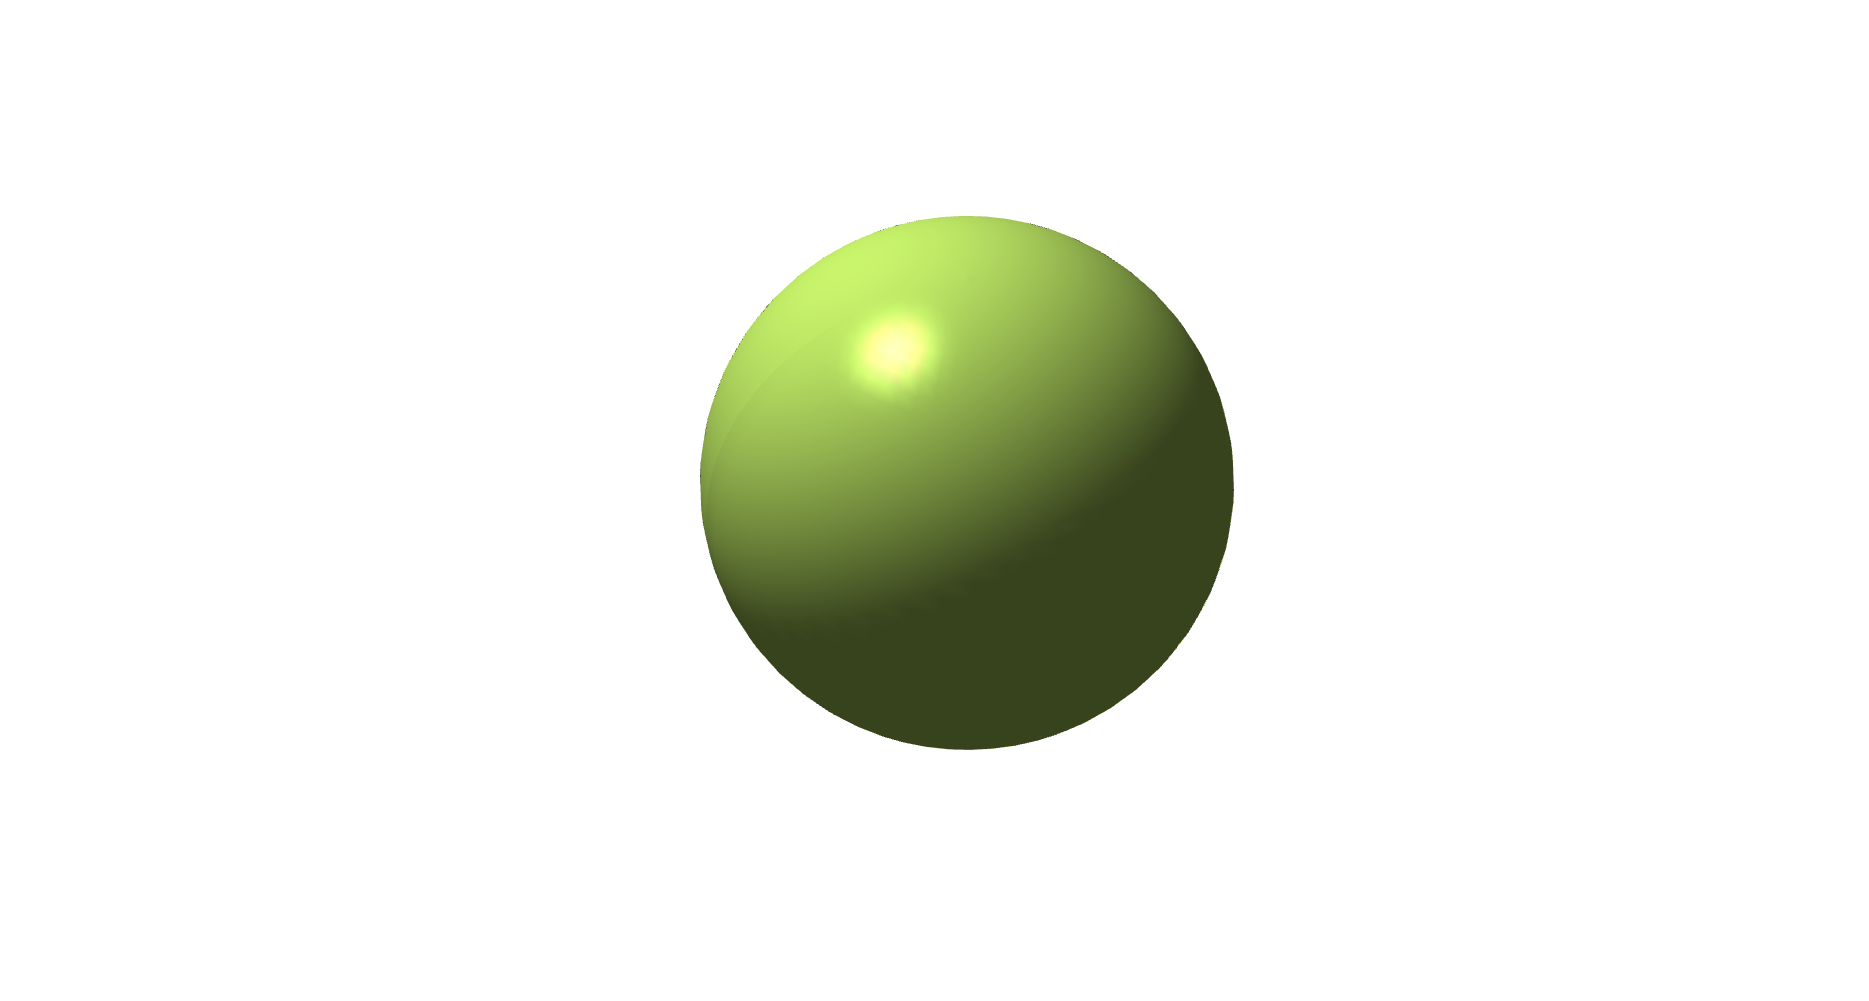
\includegraphics[width=0.2\textwidth]{./img/sphere}&
  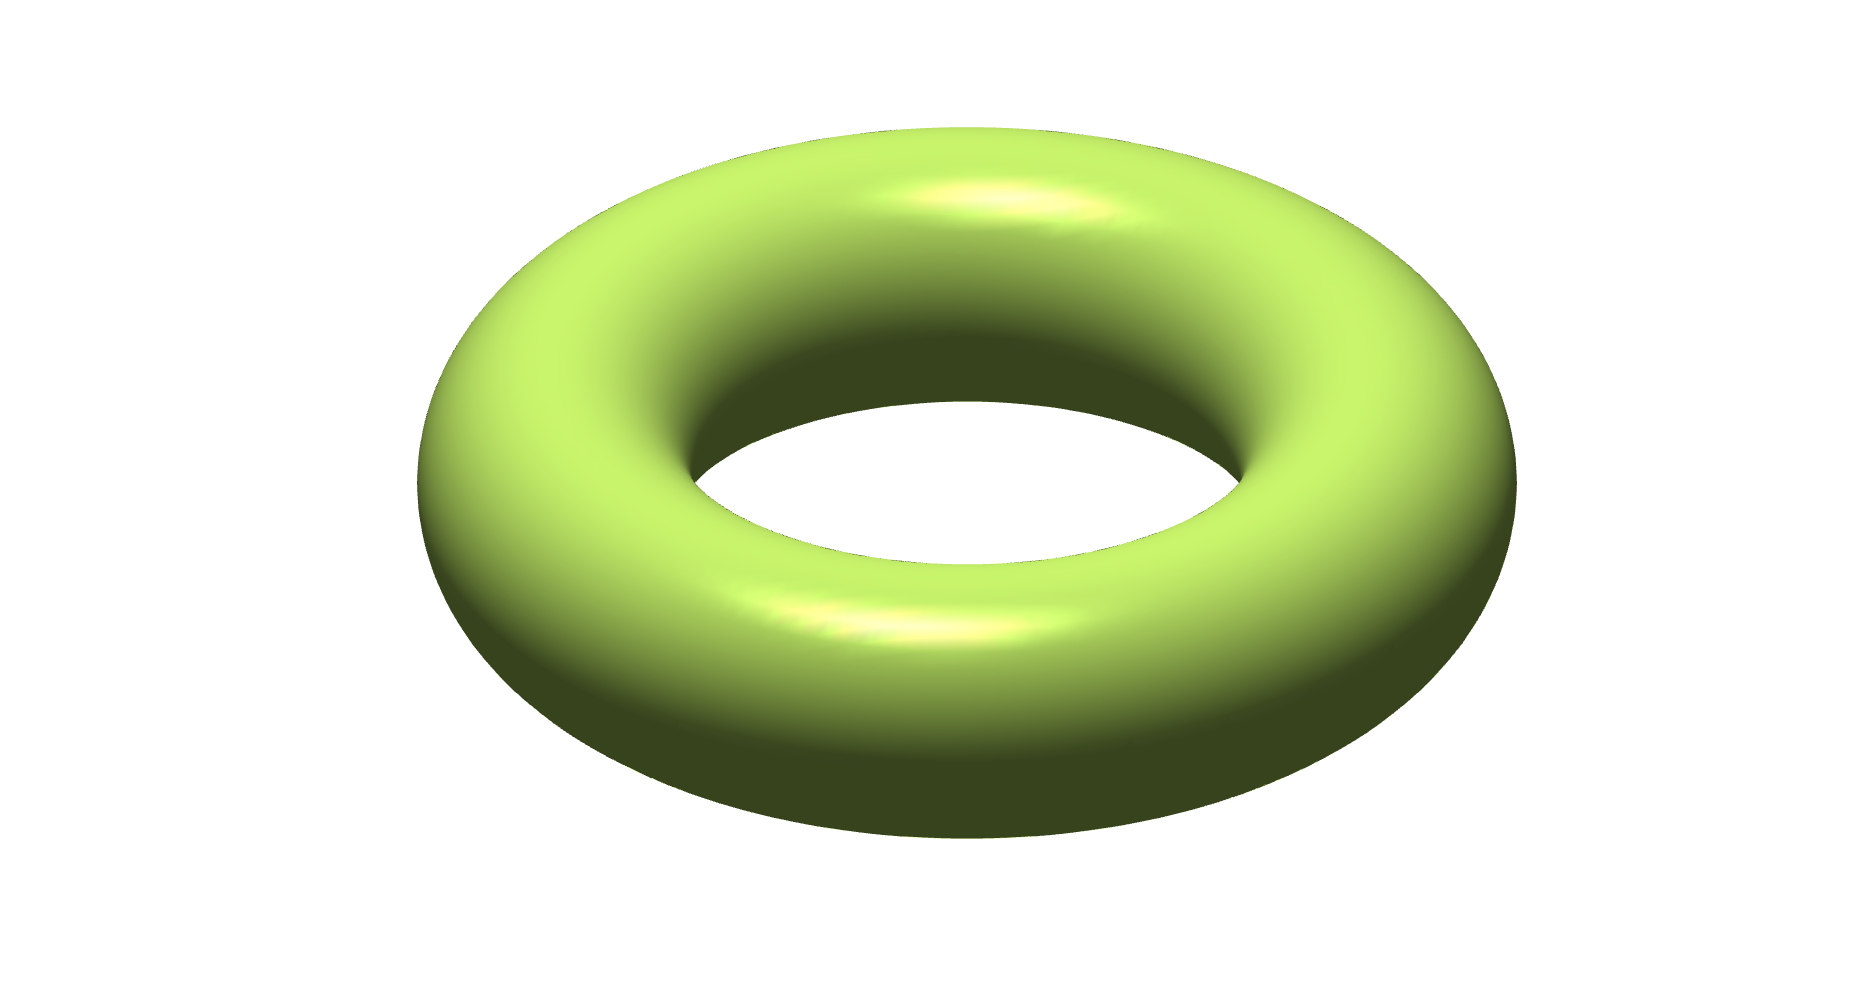
\includegraphics[width=0.2\textwidth]{./img/torus}&
  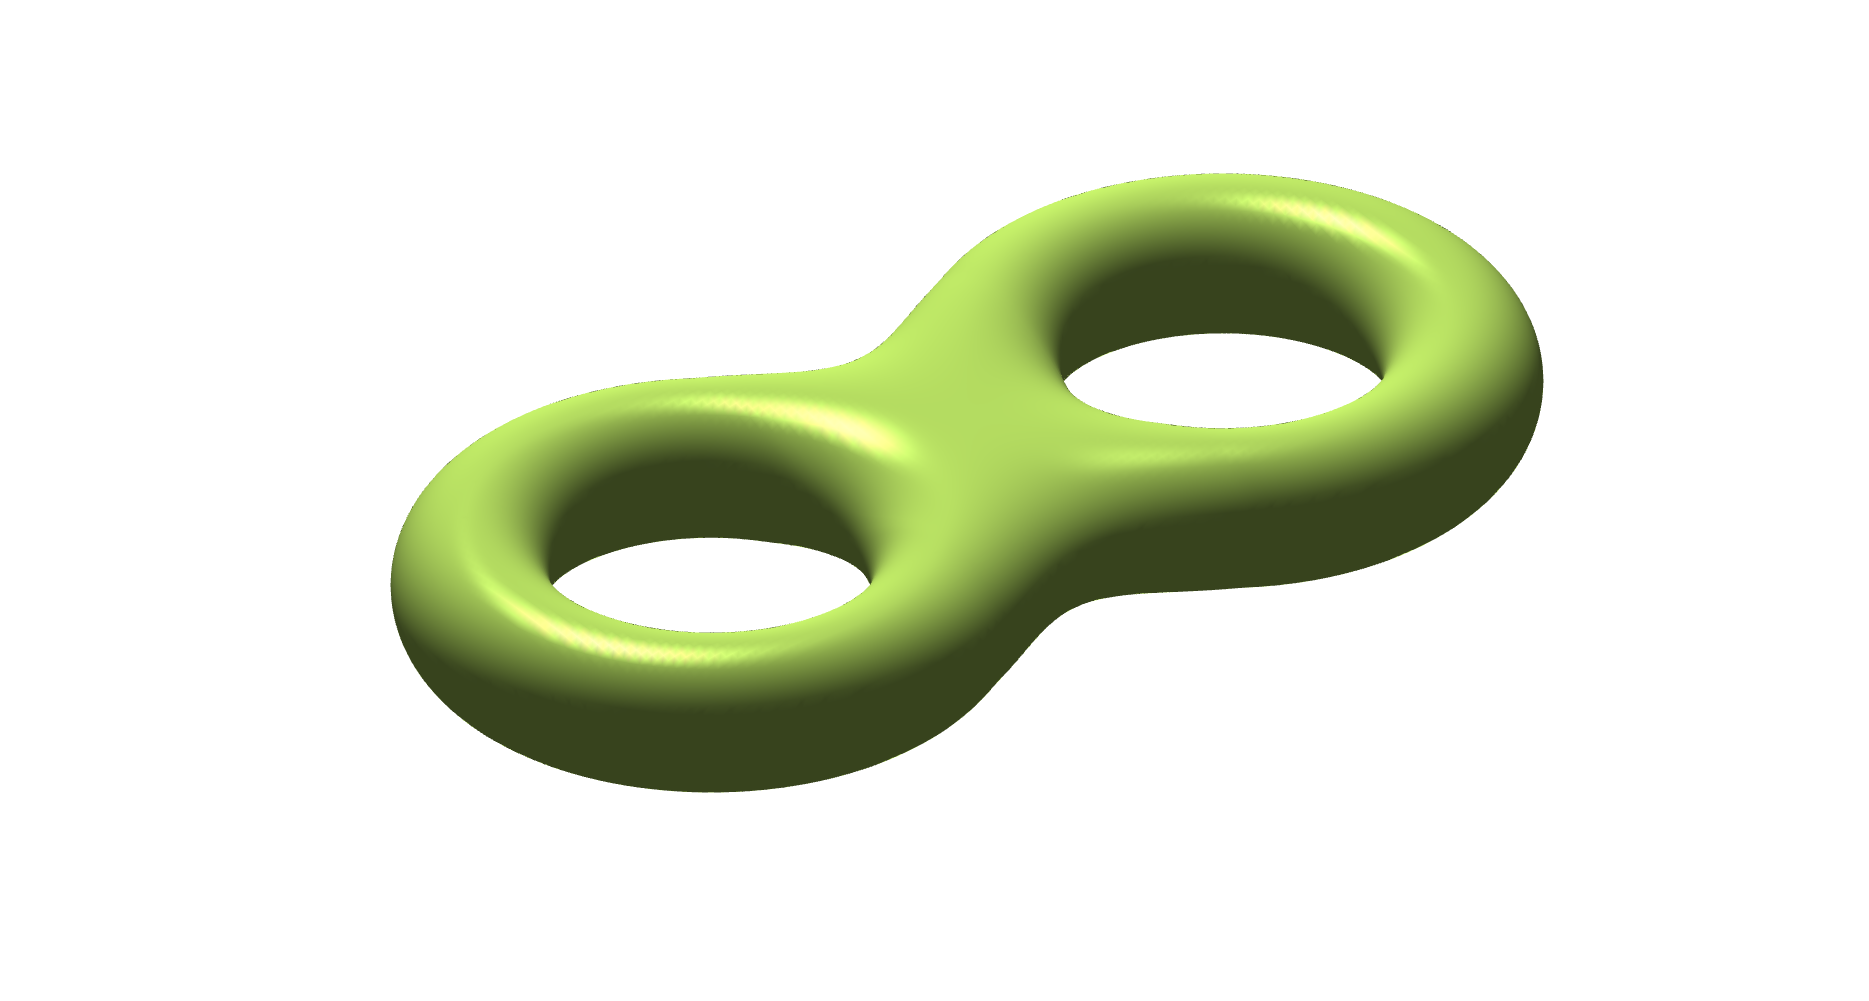
\includegraphics[width=0.2\textwidth]{./img/doubleTorus}&
  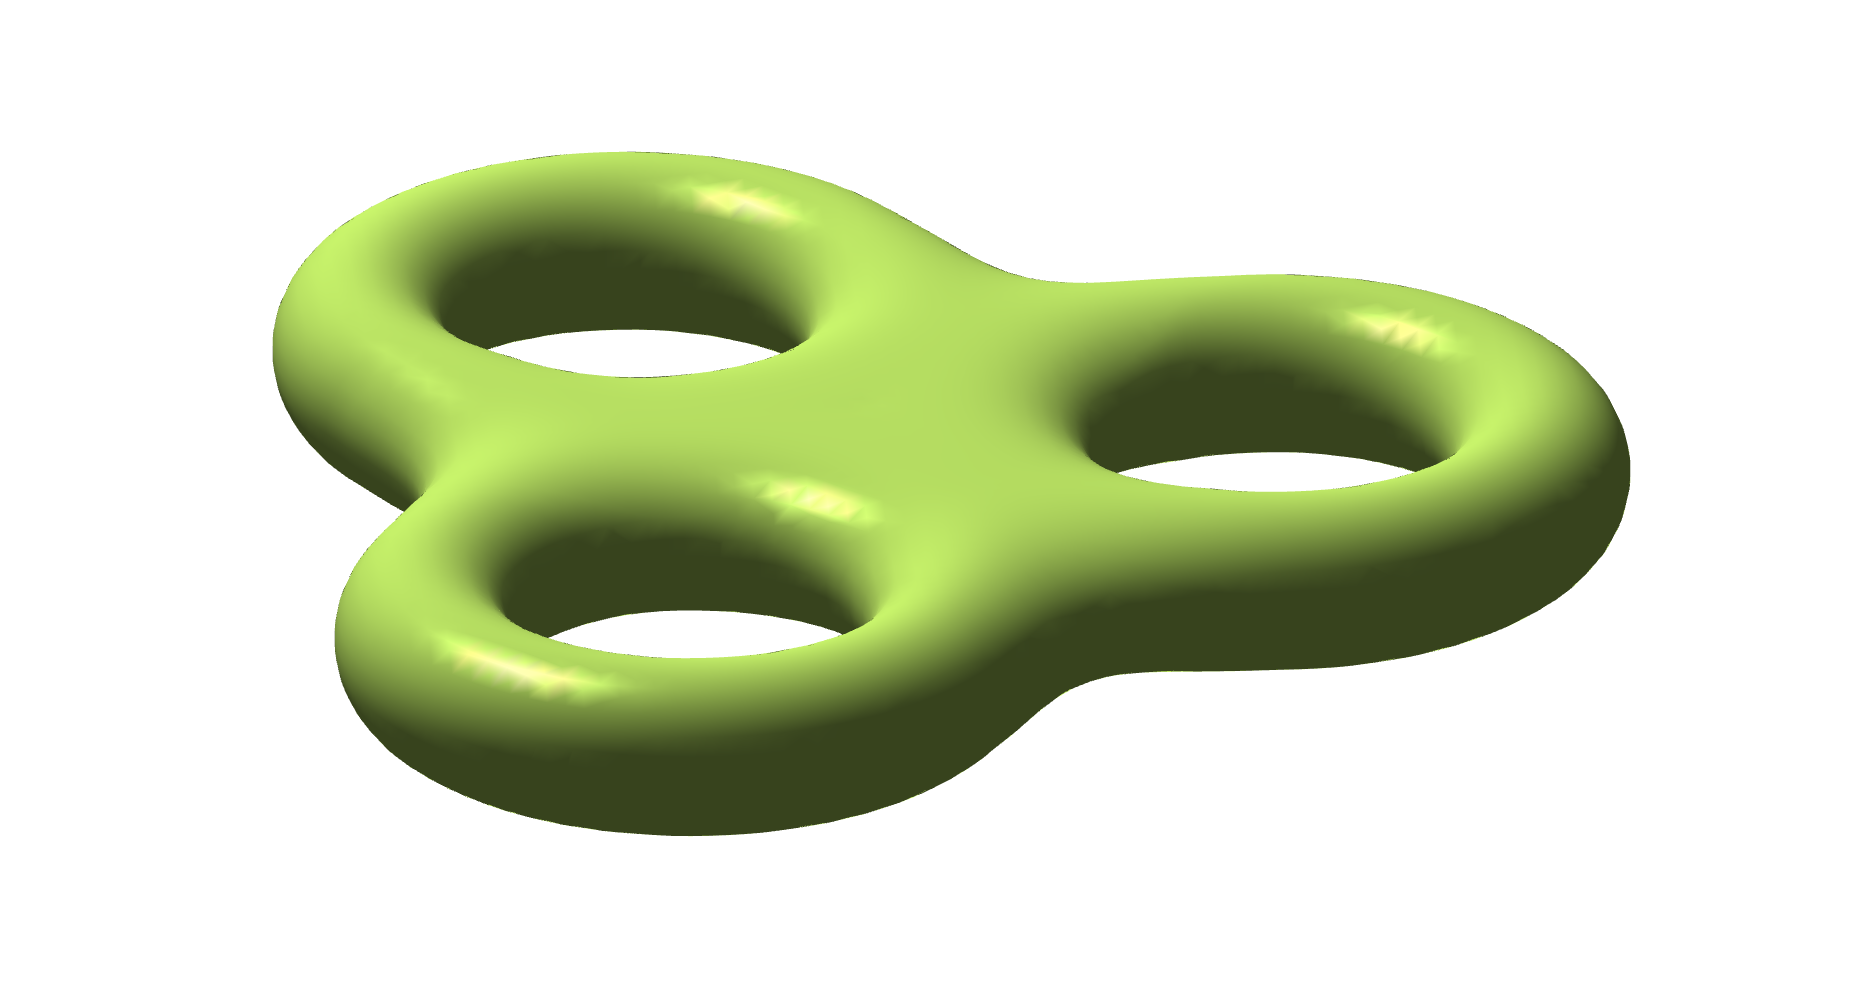
\includegraphics[width=0.2\textwidth]{./img/tripletorus}\\
  Genus 0 & Genus 1 & Genus 2 & Genus 3
 \end{tabular}
 \caption{Example of surfaces with different genus.}
 \label{fig:torus}
\end{figure}



% \begin{thm}
% Here is a new definition
% \end{thm}

\section{Manifold Surfaces in the Discrete Domain}
\label{sec:manif_discr}
The surface described thus far, can be discretized through the notion of a simplicial complex.
Recall that $k + 1$ distinct points $v_0, \dots, v_k \in \mathbb{R}^n$ are \emph{affinely independent} if a set of real numbers $\{c_0, \dots, c_k \}$ exists, such that the following equations:
\[
\sum_{i=0}^k{c_i v_i} = 0 \qquad \text{and} \qquad \sum_{i=0}^k{c_i} = 0
\]
are valid if and only if   $c_0 = \dots = c_k = 0$. 


\begin{mydef}
 \textbf{$k$-simplex}  
 Let $\{v_0, \dots, v_k\}$ be a set of affinely independent points. The simplex spanned by this set of points is their convex hull
 \[
 \sigma = [v_0, \dots, v_k] = \left\{ \sum_{i=0}^{k}{t_i v_i} : t_i \geq 0 \quad \text{and}  \sum_{i=0}^{k}{t_i} = 1\right\}.
 \]
\end{mydef}
In the previous relation, the values $t_i$ represent the barycentric coordinates of $v_i$ in the simplex, and each point in $\{v_0, \dots, v_k\}$ is named vertex (see Appendix \ref{app:barycentric_} for an in-depth about barycentric coordinates).
Each simplex spanned by a nonempty subset of the vertices in $\sigma$ is called face, if $l\leq k$ is the cardinality of this subset, then it is called $l$-face

The simplices in \Rthree are (see Figure \ref{fig:simplices}):
\begin{itemize}
  \item point: 0-simplex, with one 0-face;
  \item segment: 1-simplex, with two 0-faces and one 1-face;
  \item triangle: 2-simplex, with three 0-faces, three 1-faces and one 2-face
  \item tetrahedron: 3-simplex, with four 0-faces, six 1-faces, four 2-faces and one 3-face
\end{itemize}

\begin{figure}[t]
\centering
\begin{tabular}{cccc}

\includegraphics[width=0.15\textwidth]{./img/simplex01}&
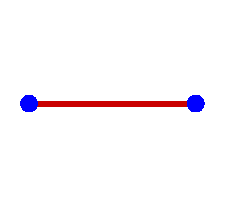
\includegraphics[width=0.21\textwidth]{./img/simplex02}&
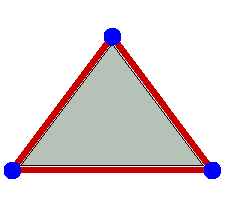
\includegraphics[width=0.21\textwidth]{./img/simplex03}&
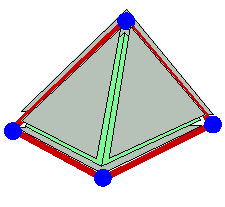
\includegraphics[width=0.21\textwidth]{./img/simplex04}
\end{tabular}
\caption{Examples of four simplex in \Rthree: 0-faces, 1-faces, 2-faces and 3-faces illustrated respectively in blue, red, gray and green}
\label{fig:simplices}
\end{figure}


\begin{mydef}
\textbf{Simplicial complex}
A simplicial complex $C$ is a finite set of simplices satisfying two properties:
\begin{itemize}
  \item any face $\phi < \sigma$ of a simplex $\sigma \in C$ is also a simplex in $C$, \ie, $\phi \in C$
  \item given two simplices $\phi, \sigma \in C$, their intersection $\phi \cap \sigma$ is a face of both $\phi$ and $\sigma$
\end{itemize}
\end{mydef}
Some examples of simplicial complexes are the triangulations of a set of points in 2D, or the tetrahedrization of a set of points in 3D.

\subsection{3D Delaunay Triangulation}
One of the most well-known 3D tetrahedrization, is the so called 3D Delaunay triangulation

\begin{mydef}
 \textbf{3D Delaunay Triangulation}
 Let $\mathit{P}$ be a set of $n \geq 4$ points in $\mathbf{R}^3$. A 3D Delaunay triangulation $T$ of $\mathit{P}$ is a 3-dimensional simplicial complex such that:
 \begin{itemize}
  \item $\mathit{P}$ is the set of vertices of T;
  \item the convex hull of $\mathit{P}$, is the union of the tetrahedra of $T$
  \item no vertex of $\mathit{P}$ is inside the circumscribing sphere of any tetrahedron of $T$.
 \end{itemize}

 
\end{mydef}

If  $\mathit{P}$ does not contain 5 cospherical points and does not contain 4 coplanar points, a 3D Delaunay triangulation of $\mathit{P}$ always exists and is unique.
Therefore, a 3D Delaunay triangulation $T$ is a particular set of tetrahedra whose vertices are the point in $\mathit{P}$; every tetrahedra has four neighbors with except for the boundary tetrahedra $\delta T$ which have a facet with no neighbors. 

A common method to assign the missing neighbor to these tetrahedra, requires to add a particular vertex $v_\infty$, named vertex at the infinity, connected to each of the boundary $\delta T$, and such that virtual infinite tetrahedra are added to the triangulation $T$. 
This step enables a more coherent implementation of the Delaunay triangulation by representing the tetrahedra and their neighboring relationships as a regular graph.

\subsubsection{Point addition and removal}
To implement an incremental reconstruction algorithm relying on the Delaunay Triangulation we will need to add points incrementally and possibly removing or moving them.

Whenever a new point has to be added into the triangulation  (the point B in Fig. \ref{fig:moving}(a)), a set of tetrahedra would conflict with it, \ie, the Delaunay property is not valid anymore (the light red triangles in Fig. \ref{fig:moving}(a)); so, this set of tetrahedra  is removed  (red triangles in Fig. \ref{fig:moving}(e)) and a new connected set that re-triangulate the hole is added to the triangulation(dark green triangles in Fig. \ref{fig:moving}(f)).

When a point has to be removed from the triangulation (the point A in Fig. \ref{fig:moving}(a)), to keep the Delaunay property, all the tetrahedra incident to that point are removed (light red triangles in Fig. \ref{fig:moving}(b)); then,  a new set of tetrahedra is added to re-triangulate the resulting hole (dark green triangles in \ref{fig:moving}(c)).

Finally, the very common approach to deal with a point moving in the triangulation, is to remove it and add it back in the new position \cite{cgal} (Fig. \ref{fig:moving}): this process is therefore composed by the two procedures described above.

\begin{figure}[t]
\centering
\begin{tabular}{cccccc}
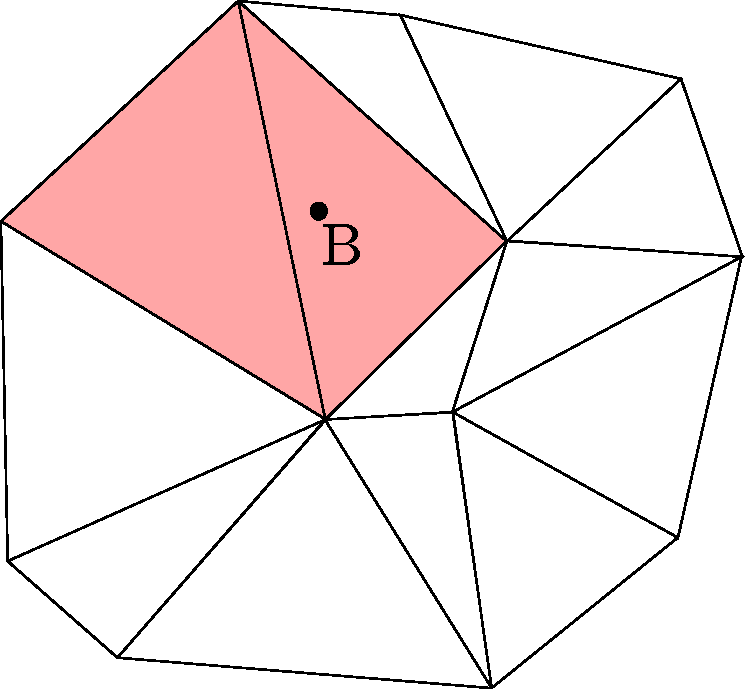
\includegraphics[width=0.25\columnwidth]{./img//delaunayExampleMoving04}&
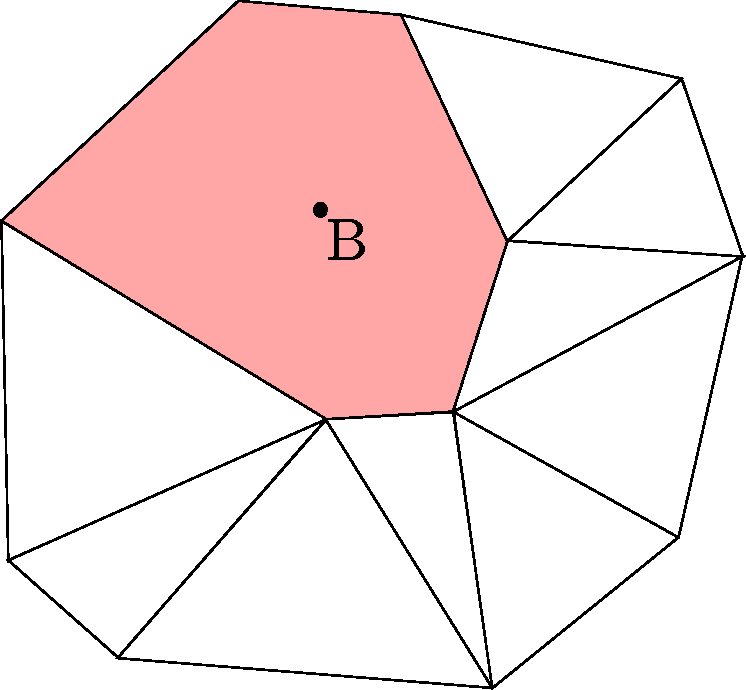
\includegraphics[width=0.25\columnwidth]{./img//delaunayExampleMoving05}&
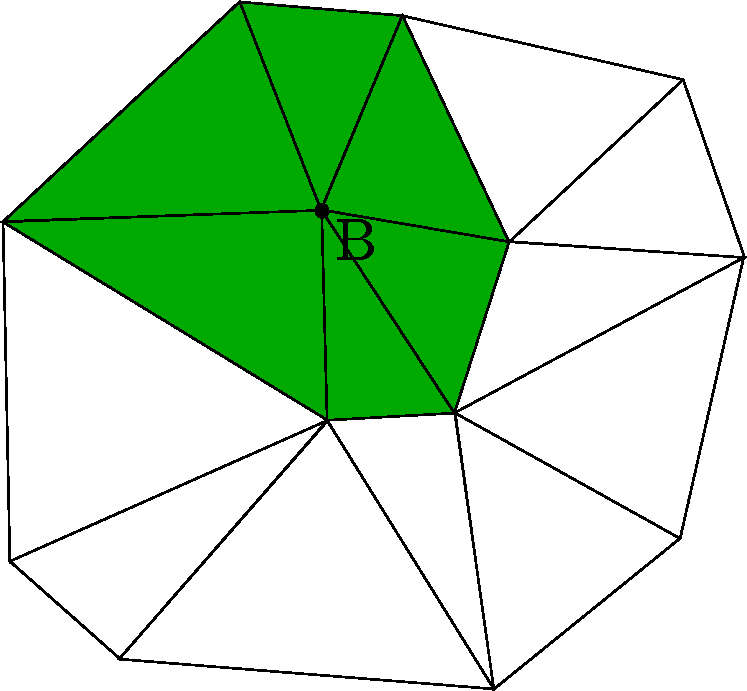
\includegraphics[width=0.25\columnwidth]{./img//delaunayExampleMoving06}\\
(a)&(b)&(c)\\
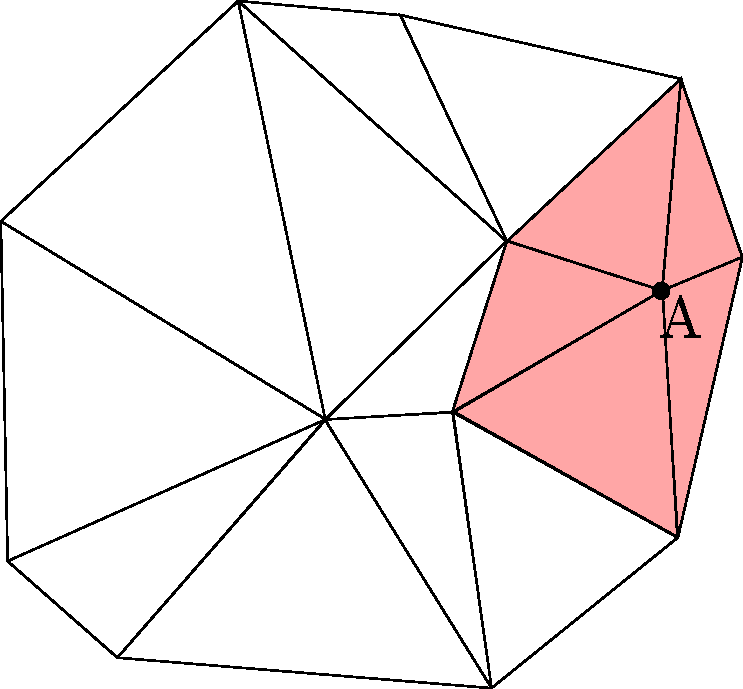
\includegraphics[width=0.25\columnwidth]{./img//delaunayExampleMoving01}&
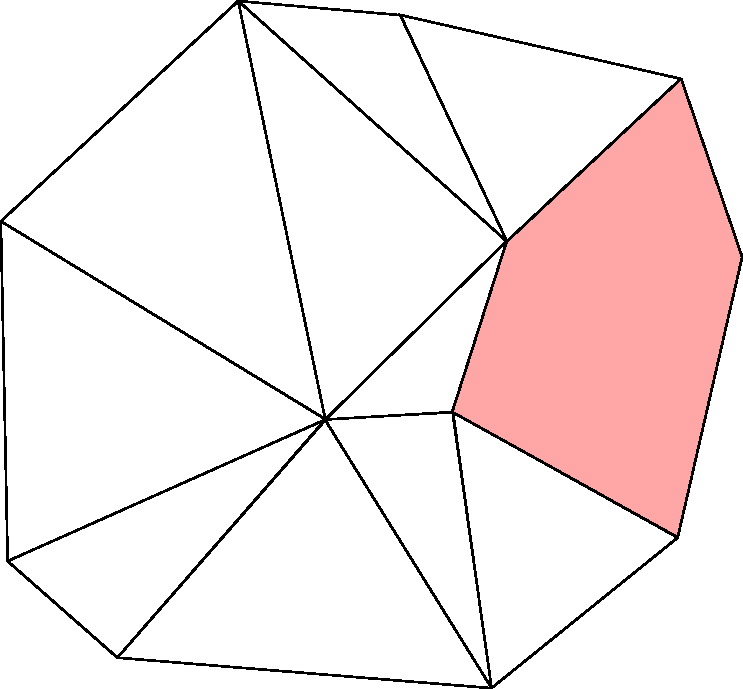
\includegraphics[width=0.25\columnwidth]{./img//delaunayExampleMoving02}&
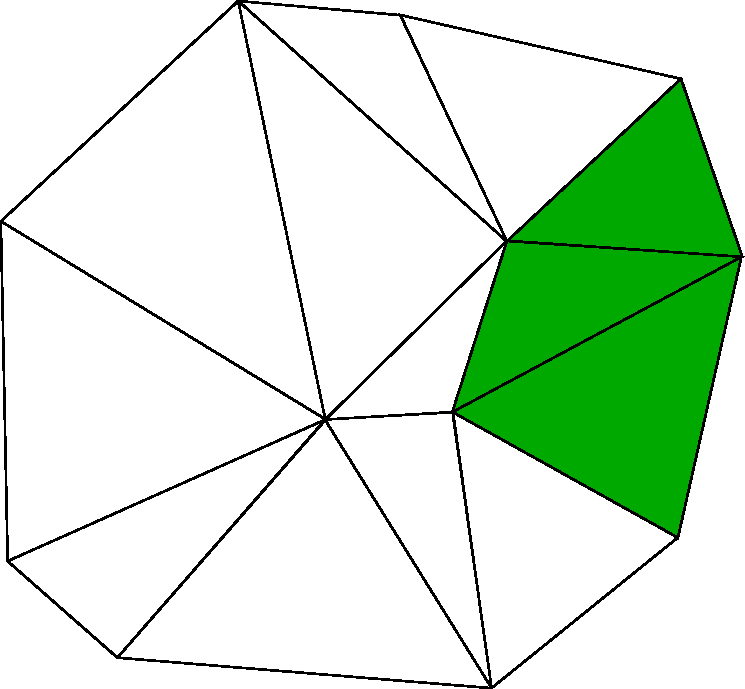
\includegraphics[width=0.25\columnwidth]{./img//delaunayExampleMoving03}\\
(d)&(e)&(f)
\end{tabular}
\caption{Point addition (\emph{a} - \emph{c}) and removal (\emph{d} - \emph{f}) in 2D case. Light red triangles depict removed and replaced with the new dark green ones.}
\label{fig:moving}
\end{figure}



\subsection{Manifold Tests}
In the first part of this thesis we aim at reconstructing the real world surface through a 2D simplicial subcomplex $\delta O$ of a Delaunay triangulation $T$ built upon a set $\mathit{P}$ of points belonging to the world 3D surface.
In particular we consider a triangulated 2-manifold.

\begin{mydef}
\textbf{Triangulated $k$-manifold}
A triangulated $k$-manifold is a simplicial complex $\delta O$ such that the union of its simplices, represented as $|\delta O|$, named polyhedron, is $k$-manifold.
\end{mydef}

In our case $k=2$, and,in the following we use the term 2-manifold meaning triangulated 2-manifold.
To check if  the union of its simplices of $\delta O$ such, represented as $|\delta O|$, is 2-manifold, given a Delaunay triangulation $T$, we define a list $O$ of tetrahedra such that $O \subseteq T$. 
The simplicial complex $\delta O$ is the boundary of $O$, and we are able to check if the relative polyhedron is $k$-manifold through the tests described in \cite{lhuillier20152}.

Let define the notion of good edges, and good vertex.


\begin{figure}
 \begin{tabular}{ccc}
  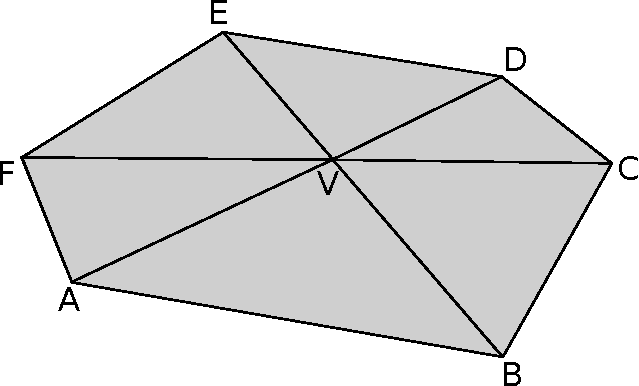
\includegraphics[width=0.28\textwidth]{./img/manifold}&
  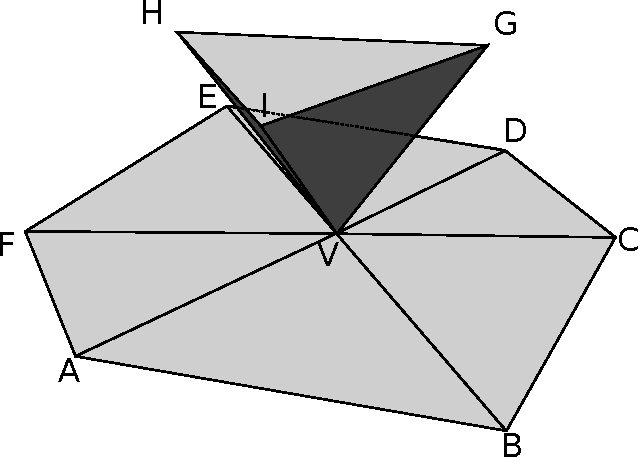
\includegraphics[width=0.28\textwidth]{./img/notmanifold1}&
  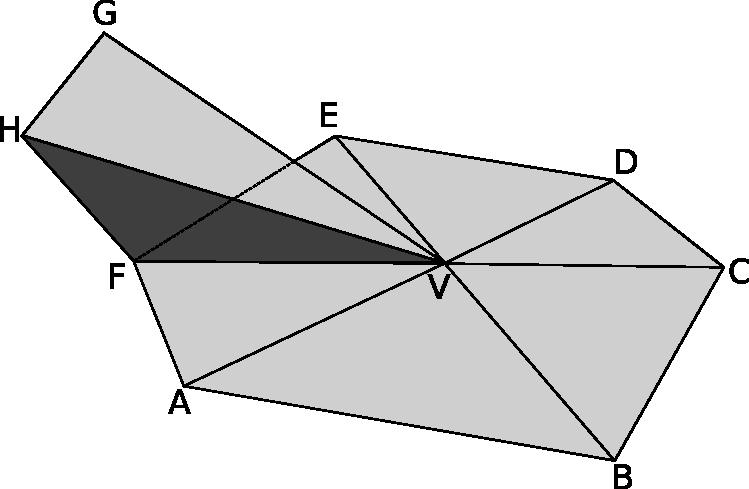
\includegraphics[width=0.28\textwidth]{./img/notmanifold2}\\
  (a) & (b) & (c)
 \end{tabular}
 \caption{Example manifold (a) and non manifold surfaces (b) and (c).}
 \label{fig:manif}
 
\end{figure}



\begin{mydef}
\textbf{Good Edges}
An edge in $\delta O$ is a good edge if it is included in exactly two triangles of $\delta O$
\end{mydef}

For instance in Figure \ref{fig:manif}(a) the edge $AV$  is a good edge, is included in triangles $ABV$ and $AFV$; while in Figure \ref{fig:manif}(c) the edge $FV$ is not, since it is included in the triangles $ABV$, $AFV$, $FHV$ and $FGV$.

\begin{mydef}
\textbf{Good Vertex}
A vertex in $\delta O$  is a good vertex if the incident triangles in $\delta O$  can be ordered as
$t_0 , t_1, \dots, t_k$  such that $t_i \cap t_{(i+1) mod (k+1)}$ is an edge $\forall i \in {0, 1, \dots, k}$.
\end{mydef}

In Figure \ref{fig:manif}(a) the vertex $V$  is a good vertex (ordering of triangles: $ABV$, $BCV$, $CDV$, $DEV$, $EFV$ and $FAV$), while in Figure \ref{fig:manif}(b) the vertex $V$ is not (no ordering guarantee the above condition).

From these two, we are able to define the following test.

\begin{thm}
  \textbf{Global Test}   
  $|\delta O|$ is a 2-manifold if and only if contains only good vertices and good edges.
\end{thm}



A second, more practical and operational test is the following


\begin{thm}
  \textbf{Vertex-Based Test}   
   $|\delta O|$ is a 2-manifold if and only if all the vertices are regular.
\end{thm}

where

\begin{mydef}
  \textbf{Regular vertex}   
   A vertex v is regular  if and only if the path of the opposite edges in the triangles having v as vertex is homeomorphic to a 2D disk.
\end{mydef}


For instance the vertex $V$ in Figure \ref{fig:manif}(a) is regular ($ABCDEF$ is a closed path and a single cycles, so is homeomorphic to a disk), while in Figure \ref{fig:manif}(b) and \ref{fig:manif}(c) the vertex $V$ is not regular since, in the former case the path $ABCDEFGHI$ is not closed, and in the latter $ABCDEFGHF$ has two cycles.


Finally we present a very useful manifold tests for incremental manifold reconstruction, originally proposed by \cite{litvinov_lhuillier_13}; by assuming $|\delta O|$ 2-manifold, the test aims at checking if the addition of one tetrahedron inside the set $O$, keeps the boundary $|\delta O|$ manifold.



\begin{thm}
  \textbf{One-tetrahedron addition test}   
  Assume that $|\delta O|$ is a 2-manifold. Let $\Delta \in T \setminus O$ and $(f,e,v)$ be a triplet representing respectively the number of triangles, edges and vertices in $ \Delta \cap \delta O$.
  $\delta (O \cup \{ \Delta \})$ is 2-manifold if and only if  $(f,e,v) \in  \{(0, 0, 0),\allowbreak (1, 3, 3),\allowbreak (2, 5, 4),\allowbreak (3, 6, 4),\allowbreak (4, 6, 4)\}$
\end{thm}
To better understand the triplets and the cases listed above see Figure \ref{fig:maniftest}: for each case we represent the tetrahedron to be tested, whose vertices, edges and facets are depicted in blue, red and green if they intersect the manifold before addition.

A similar test define if a tetrahedron subtraction keeps the manifold property valid (let note that subtracting $\Delta$ from $O$ is analogous to adding $\Delta$ to $T \setminus O$).


\begin{thm}
  \textbf{One-tetrahedron subtraction test}   
  Assume that $\delta O$ is a 2-manifold. Let $\Delta \in O$ and $(f,e,v)$ be a triplet representing respectively the number of triangles, edges, vertices in $ \Delta \cap \delta O$.
  $\delta (O \setminus \{ \Delta \})$ is 2-manifold if and only if  $(f,e,v) \in  \{(0, 0, 0),\allowbreak (1, 3, 3),\allowbreak (2, 5, 4),\allowbreak (3, 6, 4),\allowbreak (4, 6, 4)\}$
\end{thm}

\begin{figure}
 \begin{tabular}{ccccc}
  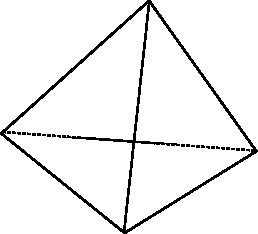
\includegraphics[width=0.15\textwidth]{./img/maniftest01}&
  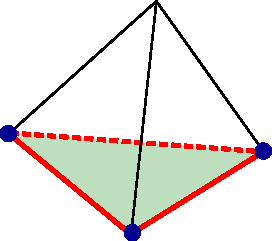
\includegraphics[width=0.15\textwidth]{./img/maniftest02}&
  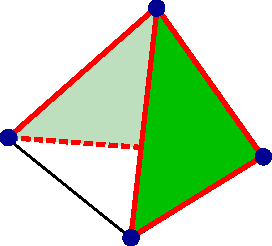
\includegraphics[width=0.15\textwidth]{./img/maniftest03}&
  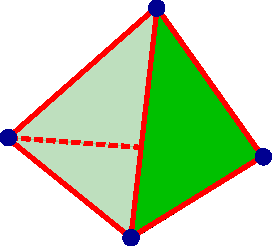
\includegraphics[width=0.15\textwidth]{./img/maniftest04}&
  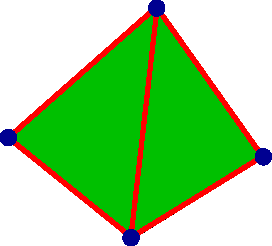
\includegraphics[width=0.15\textwidth]{./img/maniftest05}\\
  (0,0,0) & (1,3,3) & (2,5,4) & (4,6,3) & (6,6,4)
 \end{tabular}
 \caption{One Tetrahedron addition test: the figure depicts the five cases of manifold-tetrahedron intersection that lead to a positive outcome to the test; each triplet expresses the number of (facets, edges, vertices) in the intersection between the tetrahedron and the manifold before addition.}
 \label{fig:maniftest}
 
\end{figure}

\section{Mesh processing}
One of the most common data structure in the computer graphics community is the so called triangle mesh \cite{botsch2010polygon}.

Intuitively a triangle mesh is a collection of 2D triangles, their edges and vertices in $\mathbb{R}^3$. 
These triangles represent a piecewise linear surface adopted to approximate a continuous real 3D surface. 

Formally, a triangle mesh $\mathit{M} = (V,E,F)$ is a simplicial complex with a set of vertices
\[
  \mathit{V} = \{v_1, \dots, v_V\},
\]
a set of edges
\[
  \mathit{E} = \{e_1, \dots, e_E\}, \quad e_i \in \mathit{V}\times\mathit{V},
\]
and a set of faces
\[
  \mathit{F} = \{f_1, \dots, f_F\},\quad f_i \in \mathit{V}\times\mathit{V}\times\mathit{V}.
\]

The geometric embedding of the simplicial complex $\mathit{M}$ in \Rthree  is the homeomorphism $\mathit{P}$ that associates the vertices $v_i \in \mathit{V}$ with their positions $p_i$:
\[
\mathit{P} = \{\mathbf{p_1}, \dots, \mathbf{p_v}\}, \quad \mathbf{p_i}:=p(v_i) = 
\begin{bmatrix}
x(v_i)\\
y(v_i)\\
z(v_i)
\end{bmatrix}
\in \mathbb{R}^3
\]
and associates each facet $f_i\in \mathit{F}$ to a triangle in \Rthree specified by the corresponding  3D vertices.
In the following, we make no distinction between the abstract elements of the simplicial complex and their actual embedding in the geometry of \Rthree.
A 2-manifold triangle mesh is a case of Triangulated $k$-manifold.
% 
% \subsection{Barycentric Coordinates}
% Let $\mathit{t} = [\mathbf{a}, \mathbf{b}, \mathbf{c}]$ be a triangle; the position of every point $\mathbf{p} \in \mathit{t}$  can be expressed by the combination of the vertex positions:
% \[
% \mathbf{p} = \alpha \mathbf{a} + \beta \mathbf{b} + \gamma \mathbf{c}
% \]
% where 
% \[
% \alpha + \beta + \gamma = 1, \quad \alpha, \beta, \gamma \geq 0
% \]
% In Appendix \ref{app:barycentric_} we show how to compute these coordinates. %\todo{metto qui il calcolo??}

\subsection{Smoothing}
\label{sec:sm}
Mesh smoothing aims at estimating a smooth function $p$ defined on a triangular mesh.
Usually the function $p$ represents the position of the mesh vertices and the smoothing process moves it. 
Here we describe the principles of two most common approaches, for a more detailed descriptions see \cite{botsch2010polygon,taubin1995signal,taubinygeometric,sorkine2005laplacian}.
\subsubsection{Fourier transform}
Mesh smoothing can be approached as a signal analysis problem \cite{taubin1995signal}, where the smoothing operation corresponds to the application of a low-pass filter.
In the continuous 1D domain the Fourier transform is the common tool to design a low pass filter.
Given the function $p(x)$, which is the position of point $x$, and the function $P(\omega)$, which is the representation in the frequency domain, this equation connects the two representations:
\begin{equation}
p(x) = \int_{-\infty}^{\infty} P(\omega) e^{2\pi i\omega x}dx.
\label{eq:freqFourier}  
\end{equation}

Let define the inner product among two functions $f$ and $g$, to project the function $f$ in $g$ as:
\begin{equation}
\langle f,g\rangle = \int_{-\infty}^{\infty} f(x) \overline{g(x)} dx
\end{equation}
where $\overline{g(x)}$ means the complex conjugate of $g(x)$, and let the complex exponential function be:
\begin{equation}
e_{\omega} := e^{2\pi i\omega x}.
\end{equation}
Now \eqref{eq:freqFourier}  can be reformulated as follows:
\begin{equation}
p(x) = \int_{-\infty}^{\infty} \langle p, e_{\omega}\rangle e_{\omega} = \sum_{\omega = -\infty}^{\infty} P(\omega) e_{\omega} d\omega.
\label{eq:continuousFourier}  
\end{equation}
Therefore, the Fourier transform can be interpreted as the sum of the projections of $f$ on the basis functions $e_{\omega}$ for all the continuous values of $\omega$.


In the 1D domain the low-pass filter is designed such that it cuts the high frequency contributions in $p(x)$, therefore, by defining a cutting frequency $\omega_{max}$, the smoothed function $\widehat{p}(x)$ is:

\begin{equation}
\label{eq:lowpasscontinuousFourier}
\widehat{p}(x) = \int_{\omega_{max}}^{\omega_{max}} \langle p, e_{\omega}\rangle  e_{\omega}d\omega.
\end{equation}

In order to generalize this low pass filter to the 2D surface domain, we notice that $e_{\omega}$ is an eigenfunction of the Laplacian operator $\bigtriangleup$:
\begin{equation}
\bigtriangleup (e_{\omega}) = \bigtriangleup (e^{2\pi i\omega x}) = \frac{d^2}{dx^2}e^{2\pi i\omega x} = -(2\pi \omega)^2 e^{2\pi i\omega x},
\end{equation}
therefore, the 2D counterpart of the Laplacian, \ie, the Laplace-Beltrami operator, is a good candidate to generate a basis for the Fourier transformation.
In particular, we need to smooth a discrete surface, \ie, the triangular mesh, then we adopt the discrete version of the Laplace-Beltrami operator, which, for a vertex $v_i$ writes as:
\begin{equation}
\label{eq:laplacian}
\bigtriangleup p(v_i) = \frac{1}{|\mathit{N(v_i)}|}\sum_{v_ \in \mathit{N(v_i)}} w_{ij} (p(v_j) - p(v_i)).
\end{equation}
For all the vertices of the  mesh we have:
\begin{equation}
\label{eq:laplacianMatrix}
\begin{pmatrix}
  \bigtriangleup f(v_1)\\
  .\\
  .\\
  .\\
  \bigtriangleup f(v_n)
\end{pmatrix}
=
\mathbf{L}
\begin{pmatrix}
   f(v_1)\\
  .\\
  .\\
  .\\
   f(v_n)
\end{pmatrix}
\end{equation}
The eigenfunctions $e_w$ of Equation \eqref{eq:continuousFourier}, now become the eigenvectors $\mathbf{e}_{i}$ of matrix $\mathbf{L}$; they form an orthogonal basis ($\mathbf{L}$ is symmetric and positive semi-definite) of \Rn so that we write the discrete 2D version of Equation \eqref{eq:continuousFourier}:


\begin{equation}
\widehat{p}(x) = \sum_{\omega = 1}^{n} \langle p, \mathbf{e}_{\omega}\rangle  \mathbf{e}_{i}.
\end{equation}
Therefore the discrete version of the low-pass filter \eqref{eq:lowpasscontinuousFourier} becomes:
\begin{equation}
\widehat{p}(x) = \sum_{\omega = 1}^{m} \langle p, \mathbf{e}_{\omega}\rangle  \mathbf{e}_{i}.
\end{equation}
with $m<n$.

This approach to mesh smoothing allows the ideal design of a low-pass filter, the eigenvector decomposition of $\mathbf{L}$ needed to form the orthonormal basis, is an intensive process, since the number of the vertices involved, is often over the order of millions.
\subsubsection{Diffusion Flow}
A more efficient approach to deal with the smoothing is the so called diffusion flow, which acts as a Gaussian kernel directily multiplied with the 2D surface.

Let represent the points position as $p(\mathbf{x},t)$, meaning that the position evolve in (fictitious) time.
The evolution of this function is modeled as:
\begin{equation}
\label{eq:continuousdiff}
\frac{\partial p(\mathbf{x},t)}{\partial t} = \lambda \bigtriangleup p(\mathbf{x}, t),
\end{equation}
where $\lambda$ is the diffusion coefficient.
This equation implies that the evolution of the function is proportional to its Laplacian $\bigtriangleup p$.

In the discrete case, we replace the continuous Laplacian operator, with the discrete Laplacian-Beltrami one, and we discretize by $h$ the time $t$ such that \eqref{eq:continuousdiff} becomes:
\begin{equation}
\frac{\partial \mathbf{p}(t)}{\partial t} \approx \frac{\mathbf{p}(t+h) - \mathbf{p}(t)}{h}.
\end{equation}
After the integration, we obtain:
\begin{equation}
\mathbf{p}(t+h) = \mathbf{p}(t) + h \lambda \mathbf{L}\mathbf{p}(t),
\end{equation}
where $\mathbf{L}$ is the Laplacian matrix in \eqref{eq:laplacianMatrix}.
As \cite{desbrun1999implicit} suggests, the implicit Euler integration leads to a solution more stable (numerically):
\begin{equation}
\mathbf{p}(t+h) = \mathbf{p}(t) + h \lambda \mathbf{L}\mathbf{p}(t+h)
\end{equation}

The previous reasoning let us to to smooth the mesh geometry by updating, conveniently the vertices position $\{\mathbf{x}_1, \dots, \mathbf{x}_n\}$, \ie, by applying the so called \emph{Laplacian smoothing}:
\begin{equation}
\mathbf{x}_i \leftarrow  \mathbf{x}_i  + h \lambda \bigtriangleup \mathbf{x}_i , \quad i = 1, \dots, n
\end{equation}
Different discrete Laplacian-Beltrami operators $\bigtriangleup$ exist \cite{wardetzky2007discrete,sorkine2005laplacian}, but the two most common are the uniform operator and the cotangent operator.
According to the definition in Eq. \eqref{eq:laplacian}, the weights of the uniform Laplacian operator, also known as umbrella operator, are 
\begin{equation}
w_{ij} = 1 \quad iff \quad  \text{$v_i$ and $v_j$ shares one edge},
\end{equation}
% \[
% \bigtriangleup f(v_i) = \sum_{v_ \in \mathit{N(v_i)}}(f(v_j) - f(v_i)),
% \]
\ie, this operator moves each vertex by averaging the positions of the neighboring.

Instead, the so called cotangent operator, also known as mean curvature flow operator, aims at preserving the sharpness of the surface, and its weights are computed as follows:
\begin{equation}
w_{ij} = \frac{1}{2} (cot(\alpha_{ij}) + cot(\beta_{ij})) \quad iff \quad \text{$v_i$ and $v_j$ shares one edge}
\end{equation}
where $\alpha_{ij}$ and $\beta_{ij}$ are those depicted in Figure \ref{fig:cotang}
\begin{figure}[t]
  \centering
  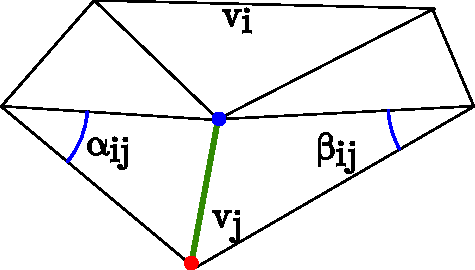
\includegraphics[width=0.7\columnwidth]{./img/laplacian}
  \caption{Cotangent Laplacian operator terms.}
  \label{fig:cotang}
\end{figure}


% \[
% \bigtriangleup f(v_i) = \frac{1}{2A_i}\sum_{v_ \in \mathit{N(v_i)}} (cot(\alpha_{ij}) + cot(\beta_{ij})) (f(v_j) - f(v_i)),
% \]
%where $A_i$ is the averaging region, 
\subsection{Self Intersections}
When dealing with mesh evolution, the self intersection problem may arise. 
As Figure \ref{fig:selfint} shows, when the vertices of the triangular mesh change their positions sometimes, it happens  that a subset of triangles intersects another set of triangles, without sharing edges or vertices. 
In this case the geometrical entity created is no longer a simplicial complex, indeed it contains a sub-mesh not visible from the outside and the normals of this sub-mesh are not meaningful anymore.
For instance in Figure \ref{fig:selfint}(a) the silhouette of the mesh moves according to the flow depicted;  the mesh evolves and self intersects  as in Figure \ref{fig:selfint}(b)  where the blue line underlines the self intersection.

The self intersections problem was faced by \cite{zaharescu2007transformesh}; the authors propose the following algorithm in order to remove the self intersections (see Figure \ref{fig:selfintalgo}).
First, the authors detect the self intersecting facets of the mesh and the collect them in the  set  $\mathit{S}$ (Figure \ref{fig:selfintalgo}(a)).
Then, they look for one random facet $f_{\text{init}}$, that is verified to be an exterior facet, \ie, not inside to the self intersection (Figure \ref{fig:selfintalgo}(b)).
From this facet $f_{\text{init}}$ they collect iteratively the adjacent triangles in the set  $\mathit{T}$ until they reach one of the triangles containing the self intersections contained in the set $\mathit{S}$ (Figure \ref{fig:selfintalgo}(c)).  
For each triangle in $\mathit{S}$ and the corresponding self intersection segment (yellow squares in the figure), they perform a constrained 2D Delaunay triangulation on their plane; among all the triangles created, they collect the exteriors one and add them to the set $\mathit{T}$.
They continue these steps until no more triangle facet has to be visited (Figure \ref{fig:selfintalgo}(d)).
Finally,  they continue to collect iteratively the triangles adjacent to those in $\mathit{T}$ not yet considered (Figure \ref{fig:selfintalgo}(e)). 
The final mesh is finally created by stitching together the triangles in $\mathit{T}$ (Figure \ref{fig:selfintalgo}(f)).

\begin{figure}
 \begin{tabular}{cc}
  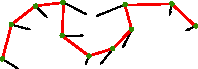
\includegraphics[width=0.45\textwidth]{./img/selfinters01}&
  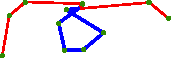
\includegraphics[width=0.45\textwidth]{./img/selfinters02}\\
  (a)&(b)
 \end{tabular}
 \caption{Example of self-intersection: a mesh evolves according to the vector flow illustrated in (a); the outcome (b) is a self-intersecting mesh (blue lines).}
 \label{fig:selfint}
\end{figure}


\begin{figure}
 \begin{tabular}{cc}
  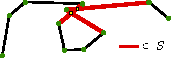
\includegraphics[width=0.45\textwidth]{./img/selfintersAlgo01}&
  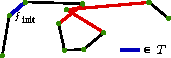
\includegraphics[width=0.45\textwidth]{./img/selfintersAlgo02}\\
  (a)&(b)\\
  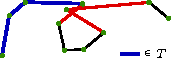
\includegraphics[width=0.45\textwidth]{./img/selfintersAlgo03}&
  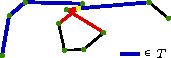
\includegraphics[width=0.45\textwidth]{./img/selfintersAlgo04}\\
  (c)&(d)\\
  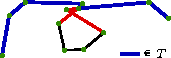
\includegraphics[width=0.45\textwidth]{./img/selfintersAlgo05}&
  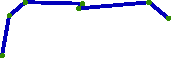
\includegraphics[width=0.45\textwidth]{./img/selfintersAlgo06}\\
  (e)&(f)\\
 \end{tabular}
 \caption{Self intersection detection and removal algorithm \cite{zaharescu2007transformesh}.}
 \label{fig:selfintalgo}
\end{figure}

\subsection{Mesh subdivision}
A very common and useful operation on meshes is the mesh subdivision.
The input is a mesh, named \emph{control mesh}, and the outputs a mesh geometrically refined and eventually smoothed.
A general mesh subdivision algorithm aims at increasing the resolution of the control mesh and recovering the underlining shape of the mesh.
New vertices are computed for each edge (edge point), facet (facet point) and vertex (new point) of the control mesh, by averaging a (usually very small) subset of neighboring vertices. 
Most algorithms moves the old vertices to approximate the underlining shape of the surface represented by the control mesh, by relying on a smoothness prior.
For instance from the control mesh in Figure \ref{fig:subdivision}(a) a general mesh subdivision algorithm adds new vertices to the red control mesh (Figure \ref{fig:subdivision}(b)), and moves them in order to recover the original black shape (Figure \ref{fig:subdivision}(c)).


\begin{figure}[tp]
\begin{center}
 \begin{tabular}{ccc}
  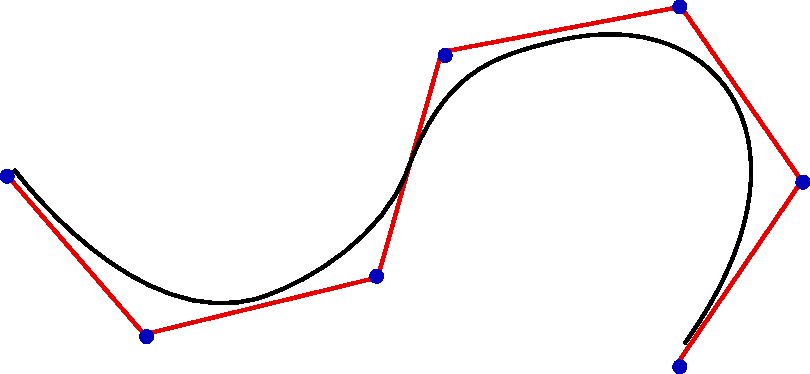
\includegraphics[width=0.28\textwidth]{./img/subdivision1d}&
  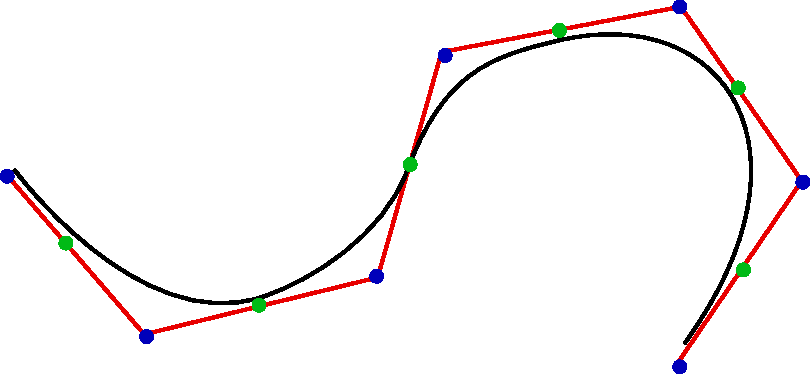
\includegraphics[width=0.28\textwidth]{./img/subdivision1d02}&
  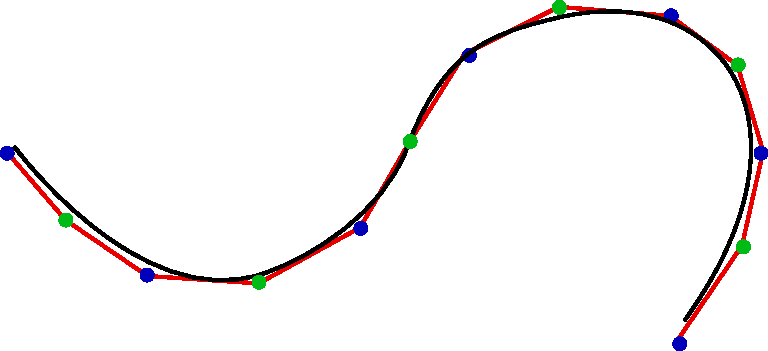
\includegraphics[width=0.28\textwidth]{./img/subdivision1d03}\\
  (a)&(e)&(f)\\
 \end{tabular}
 \caption{Mesh subdivision example: the red polyline is the control mesh, the black curve is the underlining shape.}
 \label{fig:subdivision}
\end{center}
\end{figure}

\begin{figure}[tp]
 \begin{tabular}{ccc}
 \multirow{4}{*}{
 \begin{tabular}{c}
 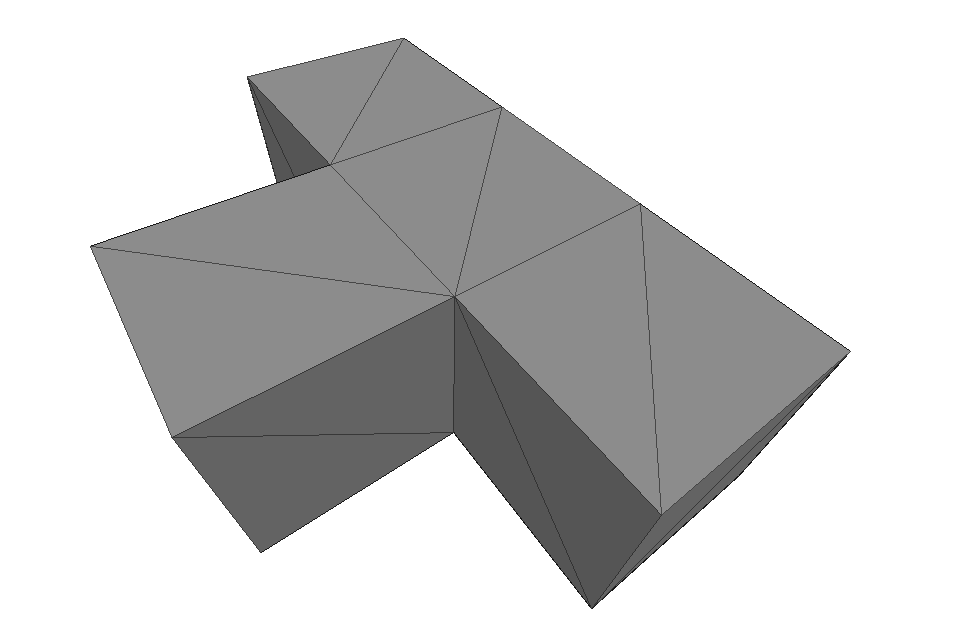
\includegraphics[width=0.22\textwidth]{./img/mesh-original}\\
 original mesh
 \end{tabular}
 }&
  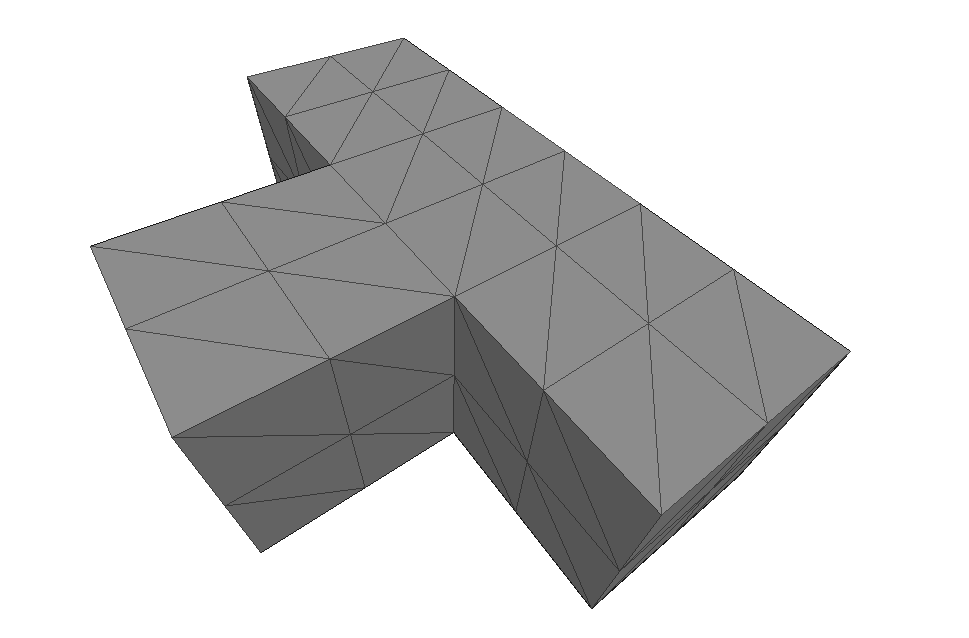
\includegraphics[width=0.28\textwidth]{./img/mesh-four}&
  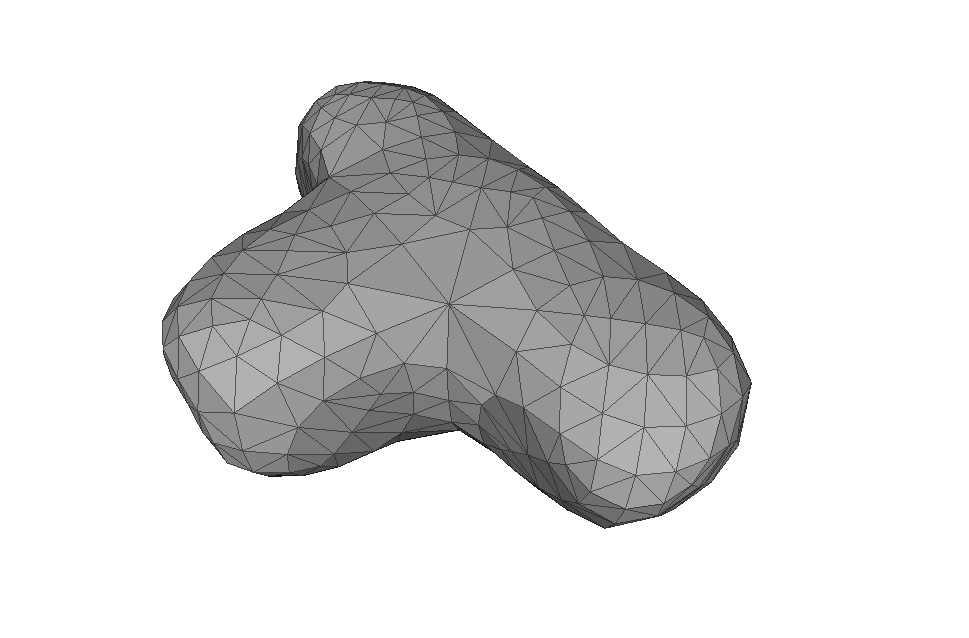
\includegraphics[width=0.28\textwidth]{./img/mesh-catmull}\\
  &one-to-four midpoint&Catmull-Clark\\&
  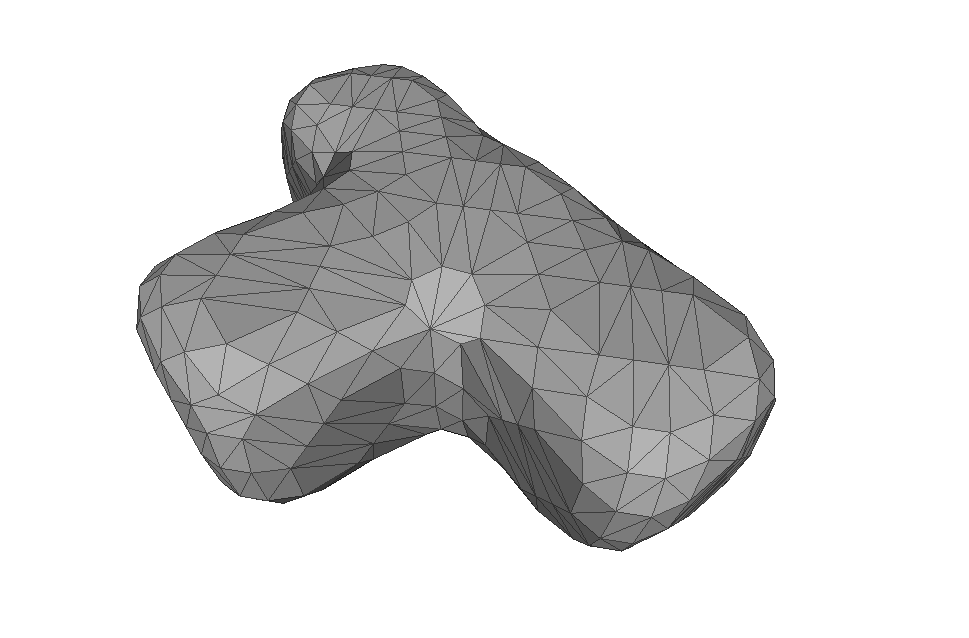
\includegraphics[width=0.28\textwidth]{./img/mesh-doosabin}&
  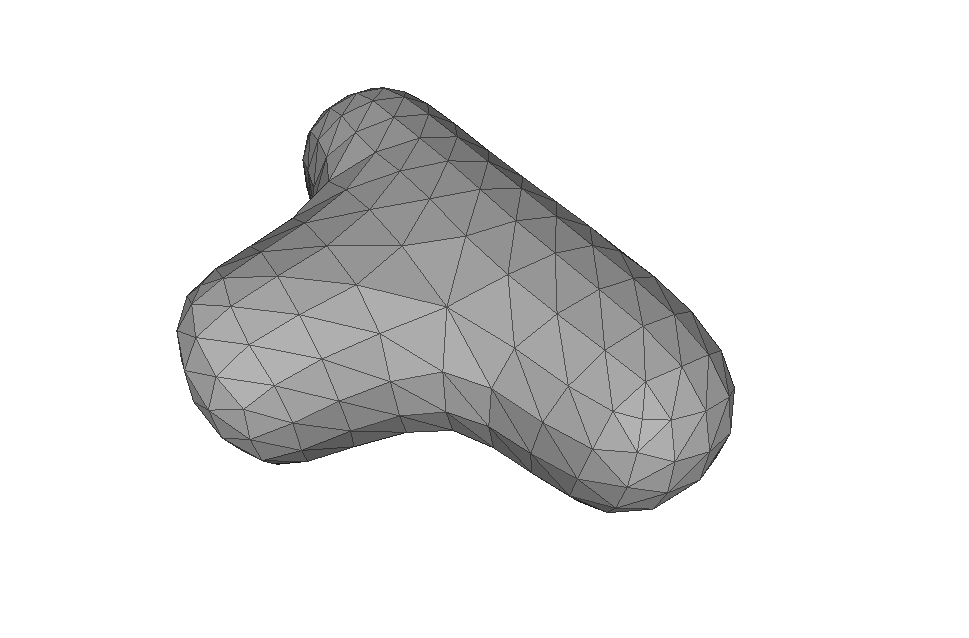
\includegraphics[width=0.28\textwidth]{./img/mesh-loop}\\
  &Doo-Sabin&Loop\\
 \end{tabular}
 \caption{Examples of different subdivision schemes.}
 \label{fig:examplsub}
\end{figure}
Several mesh subdivision algorithms have been proposed; they differ on how the vertices of the new mesh are computed. 
The CGAL library provide a package \cite{cgal:s-ssm2-15b} to fully manage the subdivision process on manifold meshes and implements the most common algorithms: one-to-four midpoint, Catmull-Clark \cite{catmull1978recursively}, Doo-Sabin \cite{doo1978subdivision} and Loop \cite{loop1987smooth}. In Figure \ref{fig:examplsub} we show how the subdivision methods act on the same mesh 

\subsubsection{One-to-four midpoint}
\label{sec:onefour}

This is the simplest, almost trivial, method to subdivide a control mesh for triangular meshes: it does not smooth the resulting mesh, but it just subdivide each triangular facet in four triangles such that it preserves the edges of the control mesh.
In this simple subdivision method no facet point are computed; the edge points are in the midpoint of each edge and the new vertex position coincides with the old vertex position.


In Figure \ref{fig:subdivisionMid} we show how this subdivision scheme acts on a single facet.



\begin{figure}[tp]
\begin{center}
  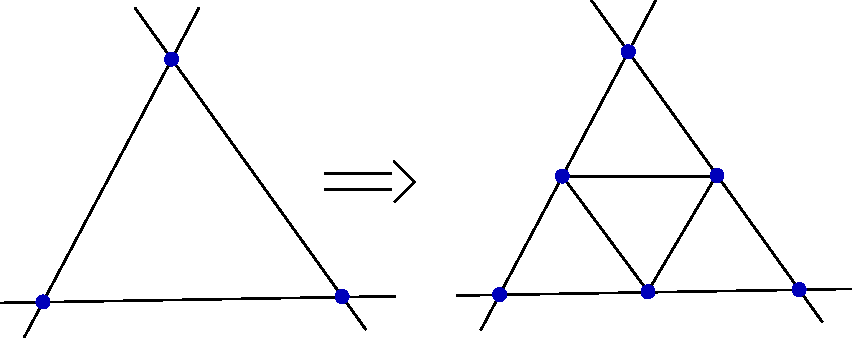
\includegraphics[width=0.8\textwidth]{./img/subdivisionMid}
 \caption{Example of one-to-four midpoint subdivision.}
 \label{fig:subdivisionMid}
\end{center}
\end{figure}

\subsubsection{Catmull-Clark}
The Catmull-Clark subdivision scheme splits the facets of the control mesh with new, and moves its old vertices in order to perform spline approximation of the surface (Figure \ref{fig:subdivisionCatmull}). It applies not only on triangular meshes, but to meshes with polygonal facets.

The algorithm adds a face-point $V_i$ for each facet $f_i$ in the average position of the corresponding polygon vertices, \eg, in Figure \ref{fig:subdivisionCatmull} $V_1 = \frac{V_1^{\text{old}} + V_2^{\text{old}} + V_4^{\text{old}} + V_9^{\text{old}}}{4}$. 
For each edge between facets $f_{i}$ and $f_{j}$ it creates a new vertex (edge-point) $E_{ij}$ averaging the position of the edge endings, and the facet-points $V_{i}$ and $V_{j}$, \eg, in Figure \ref{fig:subdivisionCatmull} $E_{13} = \frac{V_4^{\text{old}} + V_9^{\text{old}} + V_1 + V_3}{4}$.
Then, it moves each old vertex $V_i^{\text{old}}$ in a new position:
\[
V_k = \frac{(n-3)V_i^{\text{old}} + 2E + FP}{n}
\]
where $E$ represents the average position of the edge-points associated to edges incident to $V_k$ and  $FP$ is the average position of the facet-points corresponding to the $n$ facets incident to $V_k$. In the example of Figure \ref{fig:subdivisionCatmull}, 
\begin{align}
\begin{split}
    E_{sum} = E_{13}+E_{12}+E_{24}+E_{34}\\
    V_{sum} = V_1+V_2+V_3+V_4\\
    V_5 = \frac{(4-3)V_9^{\text{old}} + 2(E_{sum}/4)E + (V_{sum}/4)}{4}.
\end{split}
\end{align}




Finally, the new points are connected as follows: each face point to an edge point, which connects to a new vertex point, which, in turn, connects to the edge point of the adjoining edge, which returns to the face point.


\begin{figure}
\begin{center}
\centering
  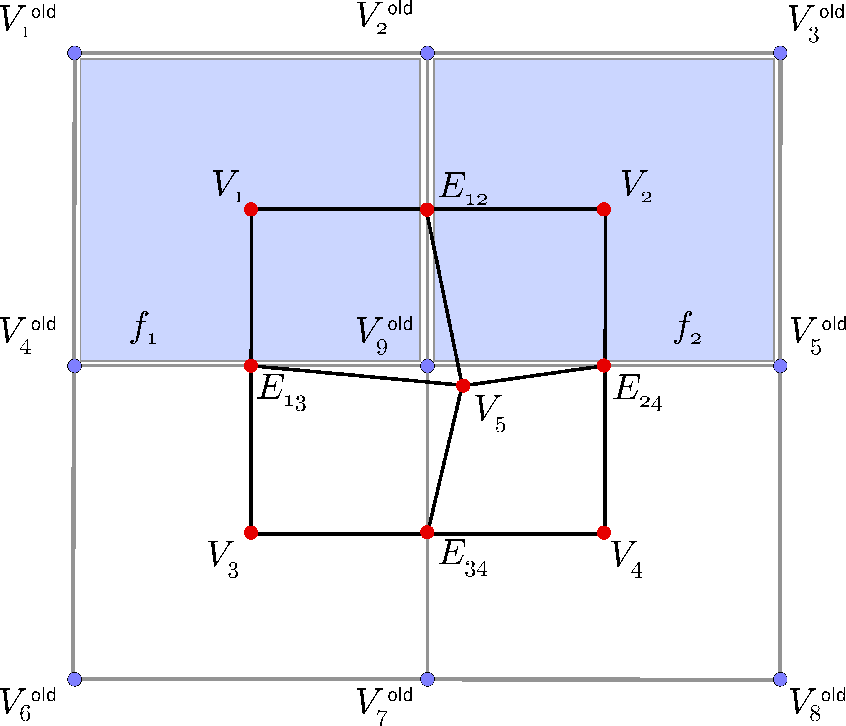
\includegraphics[width=0.8\textwidth]{./img/subdivisionCatmull}
 \caption{Example of Catmull-Clark subdivision.}
 \label{fig:subdivisionCatmull}
\end{center}
\end{figure}

\subsubsection{Loop}
The Loop scheme takes as input a triangular mesh and subdivide each triangular facet in four new smaller triangles, analogously to the one-to four scheme (Figure \ref{fig:subdivisionLoop}).
Instead of choosing the mid point as the edge point, for each edge  $e_{ij} = V_i^{\text{old}}V_j^{\text{old}}$ of the control mesh the Loop algorithm computes the corresponding edge point $E_{ij}$, by taking into account the adjoint facets $f_{a} = V_i^{\text{old}}V_j^{\text{old}}V_k^{\text{old}}$ and $f_{b} = V_i^{\text{old}}V_j^{\text{old}}V_h^{\text{old}}$. The position of the edge point $E_{ij}$ is computed as:
\[
E_{ij} = \frac{3(V_i^{\text{old}} + V_j^{\text{old}}) + (V_k^{\text{old}}) + V_h^{\text{old}}) }{8}.
\]
For instance, in Figure \ref{fig:subdivisionLoop}, $E_{12} = \frac{3(V_1^{\text{old}} + V_2^{\text{old}}) + (V_7^{\text{old}}) + V_4^{\text{old}}) }{8}$.
The new vertex point $V_i$ is computed from the old vertex and the $n$ neighboring vertices $V_j^{\text{neig}}, j = 1,\dots, n$ as:
\[
(1-s) n v_i + s \sum_{j=1}^n v_j^{\text{neig}}
\]
where, the scaling factor $s$ is:
\[
s=
\begin{cases}
  3/16 \qquad \text{if $n = 3$}\\
  \frac{1}{n} \left(\frac{5}{8} - \left(\frac{3}{8} + \frac{1}{4} cos\left(\frac{2\pi}{n}\right)\right)^2\right) \qquad \text{if $n > 3$}
\end{cases}
.
\]
No facet points are computed.

\begin{figure}
\begin{center}
\centering
  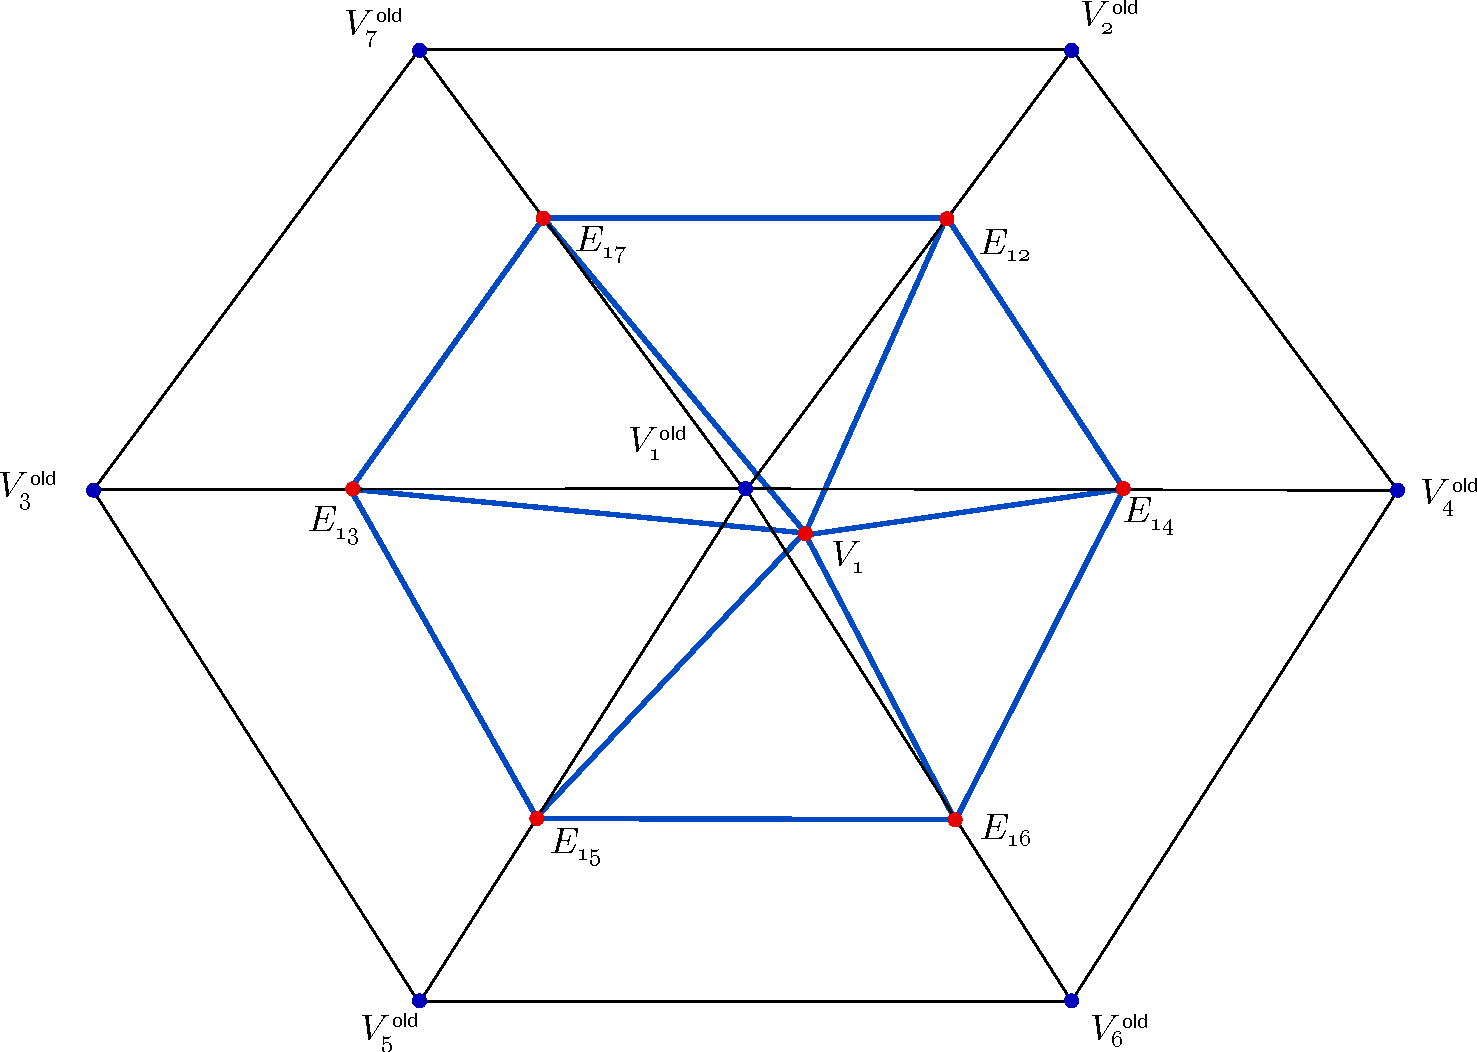
\includegraphics[width=0.8\textwidth]{./img/subdivisionLoop}
 \caption{Example of Loop subdivision.}
 \label{fig:subdivisionLoop}
\end{center}
\end{figure}

\subsubsection{Doo-Sabin}

The Doo-Sabin subdivision method, as the Catmull-Clark, applies on both triangular and quadrilateral meshes (see Figure \ref{fig:subdivisionDoo}).

The edge points $E_{ij}$ are computed as the midpoint of each edge $E_{ij} = \frac{V_i^{\text{old}} + V_j^{\text{old}}}{2}$. 
The facet points $V_i$ are centroid of the corresponding facet. 
Then, for each vertex $V_i^{\text{old}}$, a new vertex points is computed as the average of the position of $V_i^{\text{old}}$ and the facet points computed from the facets incident in $V_i^{\text{old}}$ and the edge points computed from the edges incident to $V_i^{\text{old}}$. 
For instance in Figure \ref{fig:subdivisionDoo}:
$
E_{13} = \frac{V_1^{\text{old}} + V_2^{\text{old}}}{2}
$, 
$
V_1 = \frac{V_1^{\text{old}} + V_2^{\text{old}} + V_3^{\text{old}} + V_5^{\text{old}}}{4}
$, 
$
\bar{V_1} = \frac{V_1^{\text{old}}  + V_1 + E_{13} + E_{15}}{4}
$.

Finally, the following procedure creates the new mesh. 
For each old facet, connect the new points generated inside the facet itself.
Then, for each vertex, connect the face points generated from the faces that are adjacent to this vertex. 
And for each edge, connect the new face points generated from the faces adjoining to this edge. 



\begin{figure}
\begin{center}
\centering
  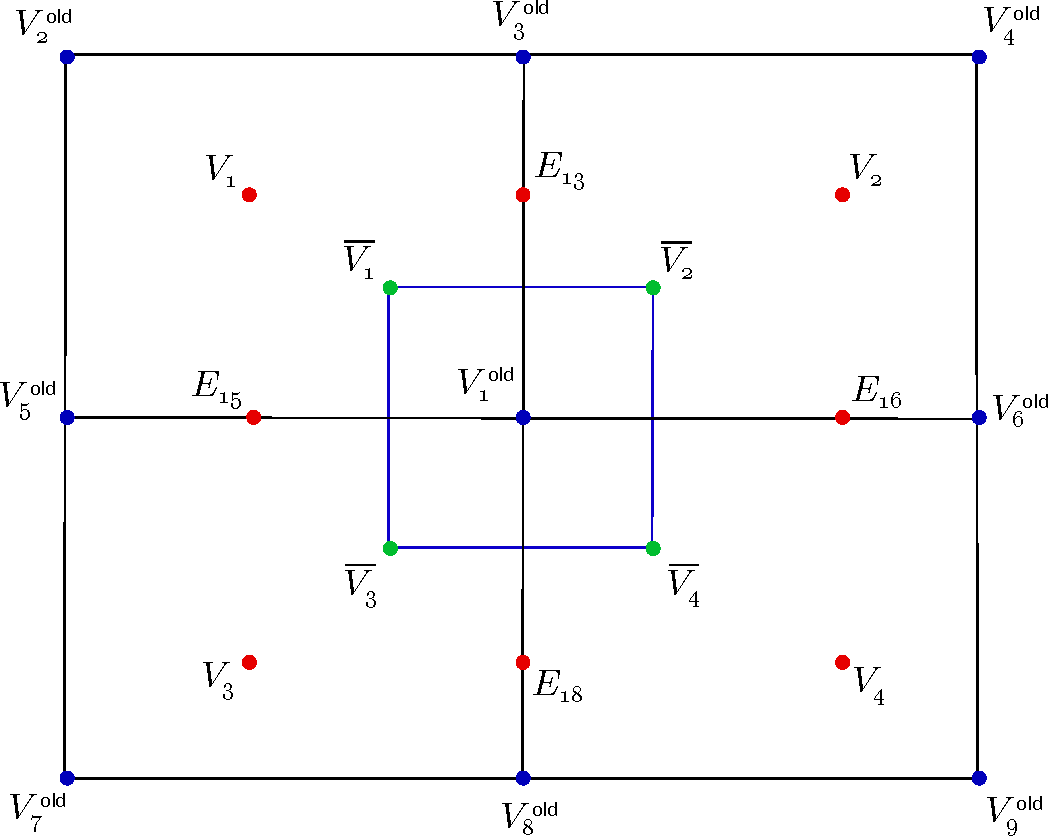
\includegraphics[width=0.8\textwidth]{./img/subdivisiondoo}
 \caption{Example of Doo-Sabin subdivision.}
 \label{fig:subdivisionDoo}
\end{center}
\end{figure}





\chapter{Camera Geometry}
\label{ch:camera}
In this chapter we provide a basic background about image formation, camera geometry, multiview geometry and OpenGL notation. 
The system proposed in this thesis builds its principles and its implementation on these tools. 
We first, describe how the image project on a standard camera, by describing the classical pin-hole model and the transformations involved. 
Then we extend the discussion to the two or multiple view case, where more than one camera look at the scene. Multiple camera are needed to reconstruct the 3D structure of a general scene.
Finally, we describe how openGL represents image formation and we provide a connection with the standard pin-hole model.


\minitoc
\newpage

\section{Image Formation}
The understanding of how the image has been generated is crucial in most computer vision applications. For instance to reconstruct the 3D geometry of the scene, a model that describes how the scene project on the images is needed. 
The classical approach to describe image formation, relies on the so called pin-hole camera model.
This model is a very effective compromise between mathematical simplicity and expressiveness.

Let assume that the world reference frame has its center $C$ in the camera center, the $Z$ axis along the principal axis of the camera, and the $Y$ and $X$ axis oriented upward and left-wise (Figure \ref{fig:pinhole}). 
We define $f$ as the focal length, that is the distance between the camera center and the image plane.
With basic geometry (see Figure \ref{fig:pinhole}(b)), the relation between  point $\mathbf{X} = \{X, Y, Z\}$ and $\mathbf{x}$ can be expressed as follows:
\begin{equation}
\label{eq:proj}
 \mathbf{x} = 
 \begin{pmatrix}
 fX/Z\\
 fY/Z\\
 f
 \end{pmatrix}
\end{equation}
The $x$ and $y$ coordinates of this point represent the position of $\mathbf{x}$ in the image plane, where the 2D reference frame is defined by the axis $x_{\text{cam}}$ and $y_{\text{cam}}$ which lay on the image plane and intersect the principal axis.
By representing $\mathbf{X}$ and $\mathbf{x}$ in homogeneous coordinates, Equation \ref{eq:proj} writes:
\begin{equation}
\label{eq:intrSimple}
 \mathbf{x}^{\text{cam}} = 
 \begin{pmatrix}
 x^{cam}\\
 y^{cam}\\
 1
 \end{pmatrix} =
 \begin{pmatrix}
 fX\\
 fY\\
 Z
 \end{pmatrix}=
 \begin{pmatrix}
 f&0&0&0\\
 0&f&0&0\\
 0&0&1&0
 \end{pmatrix} 
 \begin{pmatrix}
 X\\
 Y\\
 Z\\
 1
 \end{pmatrix}
\end{equation}

\begin{figure}[t]
\centering
 \begin{tabular}{cc}
  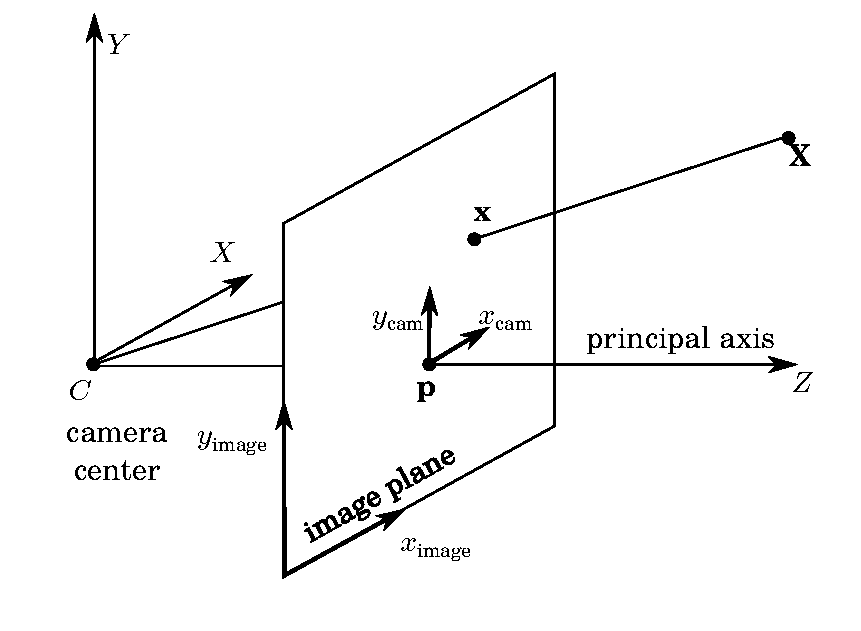
\includegraphics[width=0.45\textwidth]{./img/ch-camera/camera}&
  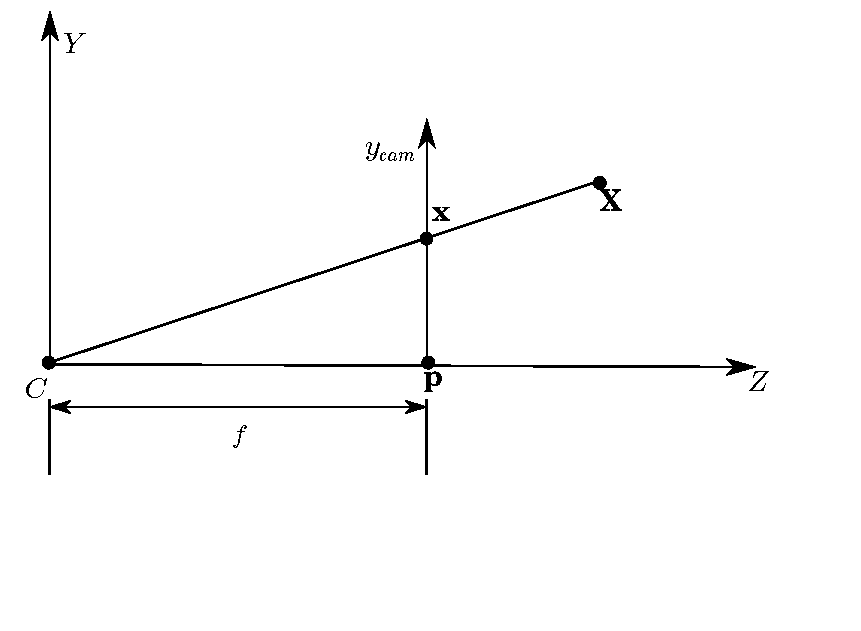
\includegraphics[width=0.45\textwidth]{./img/ch-camera/camera01}\\
  (a)&(b)
 \end{tabular}
 \caption{Pin-hole camera.}
 \label{fig:pinhole}
\end{figure}
Since an image is represented with a matrix, the coordinates $(0,0)$ are not the center of it; therefore a more practical reference frame on the image plane can be defined as in Figure \ref{fig:centercamera}. Equation \eqref{eq:intrSimple} becomes:
\begin{equation}
\label{eq:intrCompl}
 \mathbf{x}^{\text{image}} = 
 \begin{pmatrix}
 x^{cam} + p_x\\
 y^{cam} + p_y\\
 1
 \end{pmatrix} =
 \begin{pmatrix}
 f&0&p_x&0\\
 0&f&p_y&0\\
 0&0&1&0
 \end{pmatrix} 
 \begin{pmatrix}
 X\\
 Y\\
 Z\\
 1
 \end{pmatrix}
\end{equation}.
The camera 
\begin{equation}
\label{eq:kmatr}
K = 
\begin{pmatrix}
 f&0&p_x\\
 0&f&p_y\\
 0&0&1
 \end{pmatrix} 
\end{equation}
is named \emph{intrinsic camera}, and $f$, $p_x$ and $p_y$ are the \emph{intrinsic parameters}. 

\begin{figure}[t]
\centering
  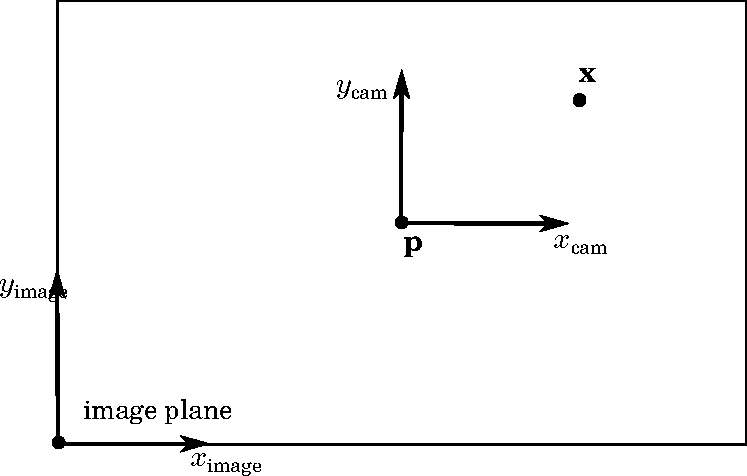
\includegraphics[width=0.8\columnwidth]{./img/ch-camera/camera02}\\
 \caption{Coordinates on the image plane.}
 \label{fig:centercamera}
\end{figure}
The assumption of a world reference frame coinciding with the camera frame is a very particular case. We now generalize the previous relation between a 3D point in the a generic world reference frame $\mathcal{W}$ and the 2D point in the image plane where the 3D point projects.
Let $C^\mathcal{W}$ be the center of the camera in the world reference $\mathcal{W}$ and  $R_\mathcal{C}^\mathcal{W}$ the rotation of the camera frame $\mathcal{C}$ with respect to $\mathcal{W}$: the matrix 
\begin{equation}
E_\mathcal{C}^\mathcal{W} = 
\begin{pmatrix}
R_\mathcal{C}^\mathcal{W} &C^\mathcal{W}\\
\mathbf{0}&1
 \end{pmatrix}   
\end{equation}
 describes the roto-translation of the camera with respect to the world reference frame.

The 3D point in Equation \ref{eq:intrCompl} is in the camera reference frame, but usually 3D points have to be expressed in the world coordinates. Therefore we rewrite the equation:


\begin{equation}
 \mathbf{x}^{\text{image}} =
\begin{pmatrix}
 K &\mathbf{0}
 \end{pmatrix} 
 \mathbf{X}^\mathcal{C}
 = 
\begin{pmatrix}
 K &\mathbf{0}
 \end{pmatrix} 
\begin{pmatrix}
 E_\mathcal{C}^\mathcal{W}
 \end{pmatrix}^{-1}
 \mathbf{X}^\mathcal{W}
\end{equation}
The matrix 
\begin{equation}
  E = (E_\mathcal{C}^\mathcal{W})^{-1} = E_{\mathcal{W}}^{\mathcal{C}} = 
\begin{pmatrix}
R_\mathcal{W}^\mathcal{C} & - R_\mathcal{C}^\mathcal{W} C^\mathcal{W}\\
\mathbf{0}&1
 \end{pmatrix}
\end{equation}
is usually referred as \emph{extrinsic matrix}: it is a roto-translation that transforms points in world coordinates to the camera reference frame.

In conclusion, the projection of a 3D point in the world to the image plane is computed as
\begin{equation}
 \mathbf{x}^{\text{image}}
 = 
\begin{pmatrix}
 K &\mathbf{0}
 \end{pmatrix} 
E
\:
 \mathbf{X}^\mathcal{W}\:=
P
\:
 \mathbf{X}^\mathcal{W}
\end{equation}
where matrix $P$ is the \emph{calibration matrix} which express both the parameters intrinsic to the specific camera (intrinsic matrix) and the position and orientation of the camera (extrinsic matrix).


\section{Multi-View Geometry}
In the reconstruction process two or more views are involved, indeed two or more 2D measurements are needed to disambiguate and estimate the 3D position. 
In this section we explain the basic principles underlying the geometry of two cameras in the projective space described thus far.
\subsection{Epipolar geometry}
The geometry between two views is known as \emph{epipolar geometry}: it depends only on the camera parameters, and is independent from the structure of the observed scene.
The epipolar geometry originates whenever two cameras look at the same scene. 
Let $C_1$ and $C_2$ be two cameras defined by the intrinsic matrices $K_1$ and $K_2$ and the extrinsic matrices $E_1$ and $E_2$.
A point $X$,  visible from both cameras, projects in the 2D point $x_1$ and $x_2$ of the $C_1$ and   $C_2$ image plane.
The camera centers $C_1$ and $C_2$, the points $x_1$ and $x_2$ and $X$ lays on the same plane $\pi$ (Figure \ref{fig:epipolar}) named \emph{epipolar plane}. 
If our information about $X$ is represented only by the projection $x_1$, we can deduce that the projection on $C_2$ of the corresponding 3D point is constrained to lay on the line $l_2$, named \emph{epipolar line}, which is the projection of the viewing ray from $C_1$ to $x_1$.



\begin{figure}[t]
\centering
  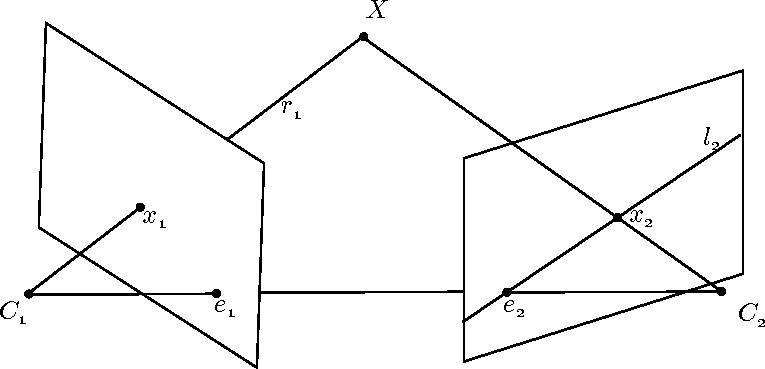
\includegraphics[width=0.8\columnwidth]{./img/ch-camera/cameraEpipolar}\\
 \caption{Two view: epipolar geometry.}
 \label{fig:epipolar}
\end{figure}
\subsection{The fundamental matrix \texorpdfstring{$F$}{F}}
The epipolar geometry of two views is synthesize into the so called \emph{fundamental matrix}, which represents a projective transformation that maps the point belonging to the image plane of one camera, to the lines of the other camera.

Given two cameras with calibration matrices $P_1$ and $P_2$, we look for the mapping between a point $\mathbf{x_1}$ located in the image plane of the first camera and the corresponding epipolar line $\mathbf{l_2}$. 
The line $\mathbf{l_2}$ is the projection on the image plane of the second camera of the line through the center $C_1$ and the point $\mathbf{x_1}$ in world coordinates, i.e., $P_1^+\mathbf{x_1}$, where $P_1^+$ is the pseudo-inverse of $P_1$ such that $P_1P_1^+ = \mathbf{I}$.
Therefore, $\mathbf{l_2}$ pass through the projection of these two points, i.e., $P_2C_1$ and $P_2P_1^+\mathbf{x_1}$, and is defined as:
\begin{equation}
 \mathbf{l_2} =  P_2C_1 \times P_2P_1^+\mathbf{x_1},
\end{equation}
where $P_2C_1$ is the epipole $e_2$. The fundamental matrix $F$ can be derived as:
\begin{equation}
 \mathbf{l_2} =  \mathbf{e_2} \times P_2P_1^+\mathbf{x_1} = [\mathbf{e_2}]_{\times} (P_2P_1^+)\mathbf{x_1} = F \mathbf{x_1},
\end{equation}
where $[\mathbf{e_2}]_{\times}$ is the skew matrix:
\begin{equation}
  [e]_{\times} =
  \begin{pmatrix}
    0   & -e_3 & e_2\\
    e_3 &   0  & -e_1\\
   -e_2 &  e_1 & 0
  \end{pmatrix}.
\end{equation}
if we know the mapping between 2D points on the two image plane, e.g., we know that $\mathbf{x_1}$ and $\mathbf{x_2}$ are the projection of the same point, the following relation, named \emph{epipolar constraint} is valid:
\begin{equation}
  \mathbf{x_2}^{T} F \mathbf{x_1} = 0.
\end{equation}
Indeed the point  $\mathbf{x_1}$ induces the epipolar line $\mathbf{l_2} = F \mathbf{x_1}$ and the point $\mathbf{x_2}$ lays on this line, i.e., $\mathbf{x_2}^{T} \mathbf{l_2} =  F \mathbf{x_1} = 0$.

\subsection{Triangulation}
In principle, if the epipolar geometry of two cameras is perfectly know, i.e., the fundamental matrix and the 2D point correspondences, the 3D point that generates the two projection is easy to recover as the intersection of the two visibility rays $r_1$ and $r_2$. 
In real cases the 2D projection is affected by noise, therefore the rays are skew and no intersection exists; the 3D position $\mathbf{X}$ needs to be estimated.

\paragraph{Linear triangulation} 
The \emph{linear triangulation} is the simplest approach to estimate the 3D point $\mathbf{X}$ given the measurements $\mathbf{x_1}$ and $\mathbf{x_2}$ in two cameras whose calibration matrices are $P_1$ and $P_2$.
The combination of the two relations $\mathbf{x_1} = P_1 \mathbf{X}$ and $\mathbf{x_2} = P_2 \mathbf{X}$ leads to a linear system in the form $A\mathbf{X} = \mathbf{0}$. 
For the first camera, we can rewrite the previous relations as:
\begin{equation}
  \mathbf{x_1} \times P_1 \mathbf{X} = \mathbf{0} \rightarrow 
  \begin{cases}
    x_1(\mathbf{p_1}^{3T}\mathbf{X}) -    (\mathbf{p_1}^{1T}\mathbf{X}) = 0\\
    y_1(\mathbf{p_1}^{3T}\mathbf{X}) -    (\mathbf{p_1}^{2T}\mathbf{X}) = 0\\
    x_1(\mathbf{p_1}^{2T}\mathbf{X}) - y_1(\mathbf{p_1}^{1T}\mathbf{X}) = 0
  \end{cases}
\end{equation}
where $P_1 = \begin{smallmatrix}(\mathbf{p_1}^1 \\ \mathbf{p_1}^2\\ \mathbf{p_1}^3)\end{smallmatrix}$ and $P_2 = \begin{smallmatrix}(\mathbf{p_2}^1 \\ \mathbf{p_2}^2\\ \mathbf{p_2}^3)\end{smallmatrix}$.
An analogous relation can be written for the second camera.
The resulting system:
\begin{equation}
  \begin{pmatrix}
    x_1\mathbf{p_1}^{3T} -    \mathbf{p_1}^{1T}\\
    y_1\mathbf{p_1}^{3T} -    \mathbf{p_1}^{2T}\\
    x_1\mathbf{p_1}^{2T} - y_1\mathbf{p_1}^{1T}\\
    x_2\mathbf{p_2}^{3T} -    \mathbf{p_2}^{1T}\\
    y_2\mathbf{p_2}^{3T} -    \mathbf{p_2}^{2T}\\
    x_2\mathbf{p_2}^{2T} - y_2\mathbf{p_2}^{1T}
  \end{pmatrix}
  \mathbf{X} = \mathbf{0}
\end{equation}
is linear and can be solved by SVD decomposition.

\paragraph{Optimal method to minimize the geometric error}
The previous method results in the minimization of an algebraic error, while a more accurate estimation can be achieved by minimizing the geometric error, i.e., by minimizing the error directly on the domain where lays the noisy measurements.
Let $\mathbf{x_1}$ and $\mathbf{x_2}$ be two noisy measurements of the point $\mathbf{X}$ in two cameras: the noise implies that they usually do not satisfy the epipolar constraint. In order to estimate $\mathbf{X}$ we ideally look for the two points $\hat{\mathbf{x_1}}$ and $\hat{\mathbf{x_2}}$, projection of the estimate $\hat{\mathbf{X}}$ that satisfy $\hat{\mathbf{x_2}}^{T} F \hat{\mathbf{x_1}} = 0$ and  minimize the function:
\begin{equation}
\label{eq:errReproj}
  d(\mathbf{x_1}, \hat{\mathbf{x_1}})^2 + d(\mathbf{x_2}, \hat{\mathbf{x_2}})^2
\end{equation}
where $d(\cdot,\cdot)$ is the Euclidean distance. 

To find the optimal solution that minimize the reprojection error \eqref{eq:errReproj}, we need to rewrite it conveniently as a function of a single variable.

First, let notice that the constraint $\hat{\mathbf{x_2}}^{T} F \hat{\mathbf{x_1}} = 0$ implies that the point $\hat{\mathbf{x_2}}$ lies on the epipolar line $l_1$, and $\hat{\mathbf{x_1}}$ lies on the epipolar line $l_2$. We can write \eqref{eq:errReproj} as:
\begin{equation}
\label{eq:errReproj2}
  d(\mathbf{x_1}, \mathbf{l_1})^2 + d(\mathbf{x_2}, \mathbf{l_2})^2.
\end{equation}
We parametrize line $\mathbf{l_1}(t)$ by $t$  and we compute the corresponding epipolar line $\mathbf{l_2}(t)$ through the fundamental matrix $F$. Equation \eqref{eq:errReproj2} now becomes:
\begin{equation}
\label{eq:errReproj3}
d(\mathbf{x_1}, \mathbf{l_1}(t))^2 + d(\mathbf{x_2}, \mathbf{l_2}(t))^2,
\end{equation}
which is a function of a single variable $t$. 
The minimization problem can now be solved by finding the root of polynomial function \eqref{eq:errReproj3}.

\subsection{Gauss-Newton for Position Refinement}
In case of multiple cameras that see the same point $\mathbf{X}$, we want to take into account all the noisy measurements of the 3D point in order to achieve a more accurate and robust estimate of it.
Equation \eqref{eq:errReproj} for $N$ cameras becomes:
\begin{equation}
\label{eq:errReprojmulti}
\sum_i=1^N d(\mathbf{x_i}, \hat{\mathbf{x_i}})^2,
\end{equation}
where $\mathbf{x_i}$ is the measurements of the point $\mathbf{X}$ in the $i$-th camera and $\hat{\mathbf{x_i}}$ is the reprojection of $\mathbf{X}$ on the same camera $i$. By making the projection explicit:
\begin{equation}
 \label{eq:errReprojmulti2}
\mathcal{C}(\mathbf{X}) =\sum_i=1^N d(\mathbf{x_i}, P_i\mathbf{X})^2 = \sum_i=1^N ||\mathbf{x_i} - proj_i(\mathbf{X})||^2,
\end{equation}
where $proj_i(\mathbf{X}) = P_i\mathbf{X}$ is the projection function for the $i$-th camera .
Therefore, the optimal method described in the previous paragraph can not be applied.
Classical methods to optimize $\mathcal{C}$ and estimate the 3D position of $\mathbf{X}$ are the gradient descent, the Gauss-Newton and the Levenberg-Marquardt algorithms. 
They are iterative methods bootstrapping from an initial guess $\mathbf{X}_0$; at the $k$-th iteration the estimate of the parameter $\mathbf{X}$ can be written as:
\begin{equation}
  \label{eq:minim}
 \mathbf{X}_k = \mathbf{X}_{k-1} + \Delta_{k-1}.
\end{equation}
The three methods differs on how they compute the value of the update $\Delta_{k-1}$.

In the gradient descent, the update follows the decreasing direction of the function computed as the inverse of the gradient evaluated at the current value of $\mathbf{X}$:
\begin{equation}
  \label{eq:discGrad}
 \Delta_{k-1} = - \gamma \nabla {proj}(\mathbf{X}_{k-1}).
\end{equation}
where $\gamma$ is a weighting coefficient.

The Gauss-Newton method computes the decreasing direction by approximating the function with the Taylor expansion; the update becomes:
\begin{equation}
  \label{eq:gaussN1}
    \Delta_{k-1}  = \mathbf{J}_{\mathcal{C}}^{-1} \mathcal{C}(\mathbf{X}_{k-1}) = - (\mathbf{J}_{proj}^T \mathbf{J}_{proj})^{-1} \mathbf{J}_{proj}^T\mathcal{C}(\mathbf{X}_{k-1}),
\end{equation}
where $\mathbf{J}_{\mathcal{C}}=\frac{\partial \mathcal{C}}{\partial \mathbf{X}}$ is the Jacobian of $\mathcal{C}$ and $\mathbf{J}_{proj}=\frac{\partial proj}{\partial \mathbf{X}}$ is the Jacopian of the reprojection function $proj$.

Finally, the Levenberg-Marquardt method combines the two previous with a coefficient $\lambda$, also known as \emph{damping factor}:
\begin{equation}
  \label{eq:l-m}
 \Delta_{k-1} = - (\mathbf{J}_{proj}^T\mathbf{J}_{proj} - \lambda diag(\mathbf{J}_{proj}^T \mathbf{J}_{proj}))^{-1}\mathbf{J}_{proj}^T \mathcal{C}(\mathbf{X}_{k-1}).
\end{equation}
The dumping factor is usually changed for each iteration in order to act similarly to gradient descent in the neighborhood of the minimum, and similarly to Gauss-Newton when we are far from the minimum \cite{Lo05}.

The Jacobian $\mathbf{J}_{proj}$ is:
\begin{equation}
  \mathbf{J}_{proj}=\frac{\partial proj}{\partial \mathbf{X}} =
  \begin{pmatrix}
   \frac{p_{0,0}^i \cdot z - p_{2,0}^i \cdot x}{z^2} & \frac{p_{0,1}^i \cdot z - p_{2,1}^i \cdot x}{z^2} & \frac{p_{0,2}^i \cdot z - p_{2,2}^i \cdot x}{z^2}\\
   \frac{p_{1,0}^i \cdot z - p_{2,0}^i \cdot y}{z^2} & \frac{p_{1,1}^i \cdot z - p_{2,1}^i \cdot y}{z^2} & \frac{p_{1,2}^i \cdot z - p_{2,2}^i \cdot y}{z^2}\\
  \end{pmatrix}
\end{equation}
with $(x,y,z)^T = P_i \mathbf{X}$.


\section{The OpenGL Camera model}
The camera model an the relations described thus far is usually referred to as HZ (Hartley-Zisserman) from the authors of the masterpiece of computer vision \cite{hazi04} that described and adopted this model extensively.
Other disciplines such as computer graphics adopt different conventions to describe the scene and the cameras. 
Since we developed the photometric refinement described in Chapter \ref{ch:incrDenseRef} with OpenGL \cite{opengl}, in this paragraph we describe the differences with respect to the HZ model and we derive the convenient transformations to switch from one representation to the other.

\subsection{The OpenGL rendering pipeline}
OpenGL is a rendering and computational engine that processes a 3D mesh. 
Each 3D vertex of the mesh is rendered on the screen after a sequence of transformations. In Figure \ref{fig:camtrans} we represent the transformations involved in both the OpenGL (top) and the HZ (bottom) models.

First, the coordinates of a 3D vertex are transformed from model to world through the model matrix. 
In computer graphics is often useful to decouple the model and the world frame in order to have the possibility to move one mesh object, without changing the camera position. 
In our case, the model of the scene is static, therefore, in the following we can overlook this matrix by assuming it as an identity.

The View matrix has a very similar meaning as the extrinsic matrix of the HZ model: it represents the roto-translation from the world to the camera. This transformations let the vertex coordinates to be expressed in the so called eye coordinates, which almost corresponds to the camera coordinates of the HZ model.

Then, a vertex is subject to the perspective and the Normalized Device Coordinates transformations.
OpenGL defines the concept of frustrum which is the portion of the scene that a camera sees (see Figure \ref{fig:perspective}(a)).
To define the extension of the frustrum, OpenGL requires the definition of the image plane position and dimension, by specifying the top, bottom, left and right coordinates and two clipping planes, orthogonal to the $z$ axis, which define the nearest and the farthest points that can be rendered, i.e. which clips the space. 
In Figure \ref{fig:frustrumTop} we show the top view of the frustrum: the darker area represents what the camera sees and what is rendered on the screen. 
The perspective projection maps the point inside the frustrum to a parallelepiped. 
Then, the NDC matrix together with the division by the fourth component w scale the parallelepiped into a cube such that each point inside it has coordinates $(x,y,z,w)$ :
\begin{equation}
 x \in [-1,1], \:
 y \in [-1,1], \:
 z \in [-1,1] .
\end{equation}

Finally, the cube is scaled and projected on the screen in order to fit the viewport dimension, i.e. the dimension of the displayed image.

\begin{figure}[t]
\centering
 \begin{tabular}{c}
  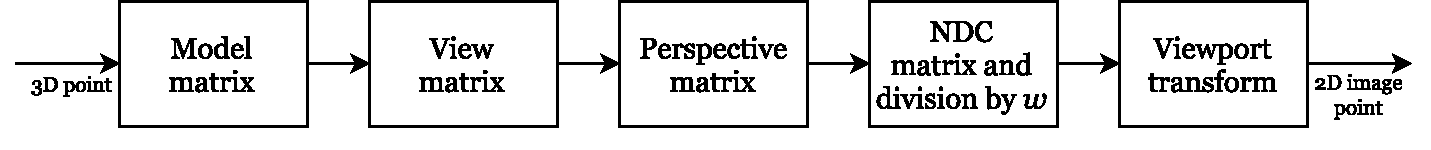
\includegraphics[height=0.1\columnwidth]{./img/ch-camera/cameraopengl-hz01}\\
  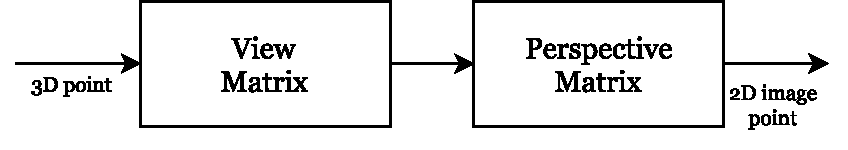
\includegraphics[height=0.1\columnwidth]{./img/ch-camera/cameraopengl-hz02}
 \end{tabular}
 \caption{OpenGL (top) and HZ (bottom) camera transformations.}
 \label{fig:camtrans}
\end{figure}

\begin{figure}[t]
\centering
 \begin{tabular}{cc}
  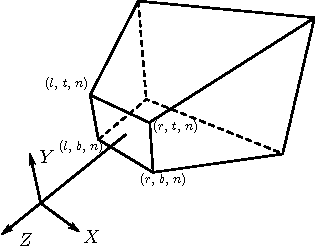
\includegraphics[width=0.45\columnwidth]{./img/ch-camera/openglcam01}&
  \includegraphics[width=0.45\columnwidth]{./img/ch-camera/openglcam02}
 \end{tabular}
 \caption{OpenGL frustrum before (left) and after (right) the perspective and NDC transformations.}
 \label{fig:perspective}
\end{figure}

\begin{figure}[t]
\centering
 \begin{tabular}{c}
  \includegraphics[width=0.78\columnwidth]{./img/ch-camera/openglcam03}
 \end{tabular}
 \caption{Top view of the OpenGL frustrum.}
 \label{fig:frustrumTop}
\end{figure}
\subsection{From Camera Calibration to OpenGL camera system}
Now we derive the openGL transformation matrices assuming the camera calibration matrix $P = K * E$ is known: let assume we have a 3D point $X = (x,y,z,w)^T$ in homogeneous coordinates, which represents a vertex of the mesh that we need to rendered on the screen with OpenGL, and we aim at simulating the camera projection performed by $P$.

First, as stated in the previous section, we let the Model matrix to be the identity, since we model a static scene rather than objects moving in the world.
\begin{equation}
  model = \mathbf{I}_{4\times4}.
\end{equation}

Then, the View matrix can be derived from the extrinsics matrix:
\begin{equation}
  E =
\begin{pmatrix}
R & \mathbf{t}\\
\mathbf{0}&1
 \end{pmatrix} 
\end{equation}
and becomes
\begin{equation}
  view = E^{-1}=
\begin{pmatrix}
R^T & -R^T\mathbf{t}\\
\mathbf{0}&1
 \end{pmatrix}.
\end{equation}

The point $X$ in camera coordinates now become:
\begin{equation}
 X^{cam} = model \cdot view \cdot X.
\end{equation}



Once we know the intrinsics parameter of the camera, i.e.,  $f_x$, $f_y$, $c_x$ and $c_y$, the perspective projection of OpenGL is very similar to $K$ in Equation \eqref{eq:kmatr}:
\begin{equation}
 persp =
 \begin{pmatrix}
  f_x & 0   & -c_x    & 0\\
  0   & f_y & -c_y    & 0\\
  0   & 0   & (n+f) & n\cdot f\\
  0   & 0   & -1      & 0\\
 \end{pmatrix}
\end{equation}
where the negative sign of the third column acts to flip the z axis according to the openGL convention, which is opposite with respect to the HZ camera; then, the third row is needed to keep the ordering of the depth and to keep the transformed point between the two clipping planes.

The point after the perspective transformation is
\begin{equation}
 X^{orto} = persp \cdot X^{cam}
\end{equation}
and it represents the point that needs to be scaled to a $([-1,1], [-1,1], [-1,1])$ cube and to be clipped if outside the frustrum.

To scale all the coordinates we apply matrix:
\begin{equation}
 NDC =
 \begin{pmatrix}
  \frac{2}{r-l}   &             0   & 0               & -\frac{r+l}{r-l}\\
  0               & \frac{2}{t-b}  & 0               & -\frac{t+b}{t-b}\\
  0               & 0               & -\frac{2}{f-n}  & -\frac{f+n}{f-n}\\
  0               & 0               & 0               & 1\\
 \end{pmatrix}.
\end{equation}
After the last transformation:
\begin{equation}
 X^{clip} = 
 \begin{pmatrix}
  x^{clip}\\
  y^{clip}\\
  z^{clip}\\
  w^{clip}\\
 \end{pmatrix}
 = NDC \cdot X^{orto} = NDC \cdot persp \cdot view \cdot model \dot X
\end{equation}
a point is rendered  only if:
\begin{equation}
 \begin{cases}
  -w^{clip} \leq x^{clip} \leq w^{clip}\\
  -w^{clip} \leq y^{clip} \leq w^{clip}\\
  -w^{clip} \leq z^{clip} \leq w^{clip}\\
 \end{cases}
\end{equation}
and then normalized in the Normalized Device Coordinates system:

\begin{equation}
 X^{NDC} = 
 \begin{pmatrix}
  \frac{x^{NDC}}{w^{NDC}}\\
  \frac{y^{NDC}}{w^{NDC}}\\
  \frac{z^{NDC}}{w^{NDC}}\\
 \end{pmatrix}
\end{equation}


Finally, OpenGL engine renders and adapts the x and y coordinates to the window, which in our case has the image dimensions.









\part{Incremental Dense 3D Reconstruction}
\chapter{From Batch to Incremental 3D Reconstruction}

\section{Image formation}



3D Reconstruction represents a long-standing topic of interest in both the Computer Vision and Robotics communities.



The reconstruction in computer vision aims at estimating an as accurate as possible map of the environment


\section{Sparse Scene Structure Reconstruction and Camera Pose estimation}
Both Structure from Motion (SfM) in Computer Vision and Simultaneous Localization and Mapping (SLAM) in Robotics face the problem of reconstructing a sparse map of the environment together with the pose (position and orientation) of the camera capturing the scene.
The early researches of the two communities, focused on different aspects of such problem.
SfM aims in particular at  estimating accurately the map (structure) of a generic set of images, it had no particular time constraints and processed all the images in the same time (batch).
On the other hand, SLAM was thought to be deployed on a robot, therefore, the main goal of is to obtain a fast and accurate estimate of the robot pose with respect to the environment by processing a video sequence: the SLAM algorithms needs to perform in real-time, i.e., at the same rate of the camera, and incrementally, i.e., a new image  has to be included in the estimation as soon as it becomes available.


These different approaches to the same problem, led the researchers of the two communities to develop deeply different algorithm relying on different estimation tools.
Classical Structure from Motion algorithms \cite{triggs2000bundle,sibley2009adaptive,wu2011multicore} extract a set of 2D points for each image with a descriptor associated, such as SIFT \cite{sift} or ORB \cite{orb}, or others, then they find the correspondences of these 2D point among all the images that are generated by the same 3D point. Bootstrapping from an initial guess, they globally optimize the pose of the camera and the 3D points position, by minimizing the error between the 2D points (the measurements) and the the projection of the current estimate of the 3D points on the cameras.
If we deal with $n$ cameras, $k$ 3D points, we express $x_{ij}^{2D}$ the measurement of point $i$ in image $j$, and $\Pi_j(x_i^{3D})$ projects the 3D point $i$ on the image plane of the $j$-th camera, SfM aims at minimizing the following:
\[
\sum_{k}^{i=0}\sum_{n}^{j=0}||x_{ij}^{2D} - \Pi_j(x_i^{3D})||^2.
\]
It is usually minimized by Gauss-Newton or Levenberg-Marquardt algorithms, and the process is usually named as Bundle Adjustment, since the minimization process adjusts the bundles of camera-to-point, by moving the camera poses and 3D point positions. This estimation usually requires a big computational effort.


Instead, the SLAM approach \cite{davison2007monoslam,ceriani2014single,grasa2011ekf}, classically adopts a different point of view, focusing on the efficiency of the estimate, and so, it uses a different estimation tool, i.e., the Extended Kalman Filter (EKF) which estimates iteratively a state, composed by the camera pose with respect to the world together with the map of the environment, by incorporating the new measurement and marginalizing the old camera poses.  


Thanks to the Parallel Tracking and Mapping (PTAM) algorithm, proposed in \cite{klein_murray07}, these two approaches become closer and closer. PTAM proposed a SLAM system that adopts the bundle adjustment optimization: it decouples the fast tracking process, i.e., the camera pose estimation, and the slow mapping processes in two parallel thread.  
The tracking processes each frame of the video sequence while the mapping works only on keyframes. 
This new paradigm, named keyframe-SLAM, gain more and more interest in the robotics community, such that it become more popular with respect to the filtering approach \cite{strasdat2010real}.
Moreover, the improvements on the bundle adjustment optimization process proposed in \cite{kaess2008isam},  the formalization of the SLAM problem as a factor graph\cite{thrun2006graph}, and the optimization libraries g2o \cite{kummerle2011g} and GTSAM \cite{dellaert2012factor} led the researchers to move from the EKF estimation to keyframe slam based on bundle adjustment \cite{strasdat11,sunderhauf2012towards,johannsson2013temporally}. 

% LSD-SLAM

In conclusion both SfM and SLAM algorithms are able to estimate the pose of the cameras and a point cloud representing the map of the environment: the former handles a generic set of data while the latter deals with a video sequence. 
In this thesis we rely on these points and cameras estimation and we provide a system able to handle a video sequence, or a set of subsequent images, that build a very accurate, continuous and dense mesh map of the environment, exploiting the advances in Multi-View Stereo and incremental reconstruction from sparse points.

\section{Multi-View Stereo}


A wide literature in Computer Vision focuses on reconstructing a scene directly from the images by assuming that the camera poses are known, usually estimated by a Structure from Motion algorithm.
These algorithms, known as Multi-View Stereo (MVS), aims at recovering a very detailed dense and accurate reconstruction. 
While, SfM and SLAM algorithms previously described output a sparse point cloud as a representation of the map of the environment, MVS aims at reconstructing at least the big majority of the image pixels, resulting in a very dense model of the environment.

\subsection{Tools and Concepts}
Before a review of existing approaches  in Multi-View Stereo, we present some concepts that are common in almost all algorithms.
\subsubsection{Photoconsistency}
Multi-view stereo aims at recovering 3D information from a set of calibrated images. The coherence and accuracy measure to evaluate and optimize the recovered 3D data is called photo-consistency, which measures the similarity between two image regions.
Different photo-consistency measure have been used. 
Given images $I$ and $J$ and two pixels $p_0\in I$ and $q_0\in J$. Very simple measures rely on the difference between the intensity values  $I(p_0)$ and $J(q_0)$ but, taking into account only a single value, they lack in robustness. 
Robust photo-consistency measures consider a set of neighboring  pixels around $p_0$ and $q_0$, i.e., $p_i$ and $q_j$ where $1\leq i \leq n$ and $1\leq j \leq n$. Usually the neighboring pixels form a rectangular region; common measures are:
\begin{itemize}
  \item Sum of Squared Differences (SSD): $\sum_{i=0}^{n}(I(p_i) - J(q_i))^2$
  \item Sum of Absolute Differences (SAD): $\sum_{i=0}^{n}|I(p_i) - J(q_i)|$
  \item Normalized Cross-Correlation (NCC): $\frac{v_{I,J}(p_0,q_0)}{\sqrt{v_{I}(p_0} v_{J}(q_0}}})$,
  where $\mu_{I}(p_0) = \frac{\sum_{i=0}^{n}I(p_i)}{n}$ and $\mu_{J}(q_0) = \frac{\sum_{i=0}^{n}J(q_i)}{n}$ are the two mean values of the pixels considered in image $I$ and $J$;
  $v_{I}(p_0) = \frac{\sum_{i=0}^{n}I(p_i)^2}{n} - \mu_I(p_0)^2$ and $v_{J}(q_0) = \frac{\sum_{i=0}^{n}J(q_i)^2}{n} - \mu_{J}(q_0)^2$ are the variances 
  and $v_{IJ}(p_0,q_0) = \frac{\sum_{i=0}^{n}I(p_i)J(q_i)}{n} - \mu_I(p_0) \mu_{J}(q_0)$
\end{itemize}
Low values of SSD and SAD represents high photo-consistency, while NCC is the correlation between two image regions. 
The computation of the NCC measure is more complex , but the final score is robust against linear illumination changes.


\subsubsection{Regularization}
\subsubsection{Variational methods}

Since the datasets of \cite{Seitz_et_al06} and \cite{strecha2008} were made available, dense MVS has been faced with different approaches, some of which reach very accurate results on these datasets.
It is hard to provide a unique classification of MVS algorithms since the methods proposed may differ in many aspect, such as the input assumptions, the algorithm to obtain the reconstruction, optimization methods. Following the taxonomy proposed in \cite{Seitz_et_al06}, we classify the MVS algorithms according to the representation of the model: \emph{depth maps}, \emph{volumetric},  \emph{level set} and \emph{mesh} methods. The four classes does not exist alone, by themselves, but a multi-view stereo algorithm, especially the most complex and recent ones, often propose a pipeline requiring different representations of the scene. In particular the depth maps-based algorithm usually needs a meshing step achieved by volumetric or implicit surfaces methods (level set).

\subsection{Depth Maps}
A depth map is a particular image that stores for each pixel the depth of the scene.
Usually the approaches based on this representation involve two steps: reference depth maps estimation and map merging.
Given a set of images, for each pixel $i$ of a reference image $I_{\text{ref}}$, the depth estimation aims at recovering the pixel depth, by pairwise comparing the appearance of the images in a process also known as stereo matching \cite{scharstein2002taxonomy}. 
The basic idea is to look for the most likely depth $z_i$ generated from the $i$-th pixel as depicted in Figure \todo{FIGURE}.

A very popular approach compares two images as follows: for each pixel $i$ of the reference frame, it scans the corresponding epipolar line in the second image, and looks for the pixel whose neighboring patch best matches the patch around $i$  \cite{lhuillier2002match}. 
Commonly used matching costs are the SSD (Sum of Squared Differences) or the NCC (Normalized Cross Correlation).
Some algorithms first rectify the two compared images, such that the epipolar line becomes horizontal and the scanning process becomes easier 
\cite{kang2001handling,bradley2008accurate,moons20093d}. 

Another approach named plane-sweeping \cite{collins1996space}, scans the entire 3D scene, that needs to be discretized, with a fronto-parallel plane, i.e., a plane parallel to the reference image plane where the other images are projected. For each pixel $i$ in the reference images, it compares the neighborhood patch against the corresponding patches in the set of projected images, and finally choose the depth $z_i$ corresponding to the best matching score. 
Following approaches propose the usage of planes in multiple directions in the whole scene \cite{gallup2007real} or locally \cite{sinha2014efficient}
Space sweeping approaches compares the image with more accuracy, thanks to the 3D projection, but the computational effort is very huge, even if highly parallelizable \cite{yang2003multi}.

The previous approaches outputs a very noisy depth map that needs to be smoothed conveniently. 
A elegant approach to depth map estimation process aims at minimizing the energy:
\begin{equation}
 \label{eq:depthenergy} 
 E(z) = \sum_i \phi(z_i)  + \sum_{ij} \psi(z_i,z_j)
\end{equation}
that combines the function $\phi$ encoding the photo-consistency described in the previous approaches, and a function $\psi$ defined over the neighborhood of the pixel $i$ that penalizes differences to encode a smoothness prior. The minimization of this energy usually bootstrap from the noisy depth maps and leads to a more accurate and smooth set of depth maps.

Different optimization tools have been adopted to minimize \eqref{eq:depthenergy}. In \cite{campbell2008using} the authors stores multiple hypothesis for each pixel depth, estimated with a classical stereo matching algorithm, then they optimize this initial depth map with multiple label, modeling the problem as a Markov Random Field. Other optimization adopt graph-cuts \cite{kolmogorov2002multi} or Bayesian approaches \cite{strecha2006combined,gargallo2005bayesian} or propagation belief methods often referred as patch-based methods, since they usually estimate small oriented rectangular patches in 3D from seeded high accurate points to their neighborhood \cite{fu10,goesele2007multi,Tola12,bleyer2011patchmatch,heise2013pm}.




The estimated depth maps contains redundant information (the regions of overlap) sometimes still noisy, i.e., the 3D points corresponding to the estimated depths, often occupy overlapped regions, and their accuracy may be still far from the true values, for instance in the lack of texture regions.
Some recent works address explicitly to these issues. 
In \cite{semerjian2014new} the authors estimate the depth maps as an energy minimization problem that aims at produce a edge-preserving smooth depth maps.
In \cite{wei2014multi} a coarse-to-fine approach together with propagation of the depth belief lead to clean depth maps.

Another source of redundancy comes for instance where a region is flat and each of this planar region is modeled. Moreover a dense and continuous 3D model of the scene still needs to be reconstructed.

The subsequent step is therefore the fusion of the depth maps. This step requires a different representation of the data, so we will describe depth fusion in the following paragraphs, in which the input of the algorithms will often be a set of depth maps or a point clouds, estimated from the depth maps  as in \cite{curless1996volumetric} or directly through stereo matching techniques as in \cite{bradley2008accurate,labatut2007efficient,vu_et_al_2012}.


\subsection{Volumetric}
Many MVS algorithms model the scene from a point cloud, from a depth map or directly from images, by relying on a 3D discretization of the world space.
A sub-classification of these volumetric approaches considers how the space is discretized: with voxels or with tetrahedra.


\subsubsection{Voxel-based}
A voxel is a the 3D extension of a pixel: if we partition the space in a regular 3D grid, each part, i.e., each small cube, is a voxel.
Voxel-based  algorithms are popular volumetric approach to merge depth maps or directly model from image, and performs very well in the Middelbury dataset \cite{Seitz_et_al06}.

The early approach proposed in \cite{curless1996volumetric}, and applied in \cite{goesele2006multi}, cumulates depth maps data in order to estimate a signed distance of each voxel from the scene surface; the final reconstruction is defined as the zero-crossing surface on the voxels.
The authors in \cite{zach2007globally} estimate a more robust distance function through total variation regularization with a $L^1$ norm data fidelity term.

Another very common approach to create a model out of the 3D oriented point associated with the depth maps, is the Poisson reconstruction \cite{kazhdan2006poisson}, which computes an indicator function (defined as 1 at the points inside the model,and 0  outside) as a Poisson problem from a gradient field depending on the integral of the surface normal field.
An improvement on the Poisson Surface Reconstruction was recently proposed in \cite{shan2014occluding} where the internal contours estimated on the depth map, acts to densify the depth maps and, free space constraints computed for each voxels, constrain the Poisson reconstruction in order to handle free space volumes.

A classical approach not requiring the depth map estimation, labels the voxels as free space or occupied, and is known as space carving or voxel coloring \cite{seitz1999photorealistic,kutulakos_seitz05}. 
This method starts with a voxelized volume circumscribing the scene, and all voxels are initialized as occupied (or ``matter``). Low photo-consistent voxels are marked as free space iteratively, until a fixed photo-consistency threshold is reached. The boundary between free space and matter is therefore the final model of the scene. 
This method need to make hard decision every time a voxel needs to be classified, and highly depends on the order of inspection. Moreover, the output may results in a noisy reconstruction with artifacts and outliers.
An improvement was proposed in \cite{broadhurst2001probabilistic}, in which soft constraints are adopted to label more fairly the voxels.
Finally, the authors in \cite{yang2003multi} improve the order of inspection and adds a smoothing term. 
However the reconstruction of voxel-based space carving is still noisy and not  accurate.
Space Carving, was also applied, more successfully by tetrahedron-based volumetric approach we will  review in next section.

More successful approaches to estimate a surface without depth maps, relies on global optimization of the energy defined by:
\begin{equation}
\label{eq:eqVoxel}
E(f) = E_{\text{data}}(f) + E_{\text{smooth}} (f) + E_{\text{visibility}} (f)  
\end{equation}


where $f:\mathit{P}\leftarrow \mathit{L}$ is the labeling function that associates a label $l\in \mathit{L}$ to the pixel $p \in\mathit{P}$, $E_{\text{data}}(f)$, $E_{\text{smooth}} (f)$ and $E_{\text{visibility}} (f)$ are related respectively to the photo-metric cost, the smoothness prior and the visibility constraints.

The most common optimization has been accomplished via graph cuts \cite{vogiatzis2005multi,kolmogorov2002multi,hornung2006hierarchical,furukawa2006carved,mucke2011surface,hernandez2007probabilistic}: the voxels are nodes of the graph, while the edges connect neighboring pixels and their capacity depends on the energy \eqref{eq:eqVoxel}. The boundary voxels links with the sink node of the graph, and voxels that are very likely to be inside the surface links to the source.
These algorithms needs a ballooning term to avoid the shrinking bias, i.e., the minimization tends to traverse as few as possible edges and tends to extract an empty surface. If this term is too large, then the solution tends to over-inflate, otherwise the solution collapses into an empty surface.
This limitation has been partially solved in \cite{hernandez2007probabilistic} where the ballooning term depends  from the visibility, or in \cite{mucke2011surface} by replacing it with convenient weighting of the edges. 
Recently, convex optimization have been also successfully applied and reaches remarkable results
\cite{kolev2009continuous,kolev2010anisotropic,kostrikov2014probabilistic}, they formalize the labeling problem as in the previous case, but compute the labels woth the primal-dual method \cite{mehrotra1992implementation}.




In general, voxel-based methods yields very accurate results, in particular when coupled with global optimization methods; however, their application is still limited by the huge requirement of memory, and even if attempts to make the representation more compact exist \cite{steinbrucker2014volumetric,chen2013scalable,zeng2013octree}, they are still not suitable for scalable large-scale reconstruction.
Moreover, only by including shape priors these methods are able to handle lack of texture \cite{karimi2015segment} that usually affects the depth maps.


\todo{FIGURE}.
\subsubsection{Tetrahedron-based}
\label{sec:tet-based}
A different volumetric approach discretize the space with a set of tetrahedra, usually computed via Delaunay Triangulation on a point cloud.
These methods are popular in the Computer Graphics community to reconstruct a surface from an unorganized (no adjacent among points is known) set of point \cite{amenta1999surface,amenta2001power,boissonnat1984geometric,dey2004provable,kolluri2004spectral}. 

Fewer tetrahedron-based methods with respect to the voxel-based ones, have been adopted in multi-view stereo reconstruction
\cite{faugeras_et_al_90,labatut2007efficient,salman2010surface,vu_et_al_2012,hiep2009towards,Pan_et_al09}.

They often rely on the space carving algorithm similar to the voxel coloring, but the boundar between free space and occupied parts is naturally a triangular mesh, very well-suited for further mesh refinement algorithms.

In the seminal work of \cite{faugeras_et_al_90} they apply a constrained Delaunay 3D triangulation to fit the stereo edges. They label  as free space the tetrahedra crossed by visibility triangles from the camera to the edges as the space carving of the voxel-based approaches. The authors apply several times a region growing from not-labeled tetrahedra  until all not-labeled tetrahedra have been visited. Each iteration of each region growing keeps the boundary 2-manifold. Finally, each region is labeled as matter only if contains enough vertices, otherwise is free space. 
Even if this approach address the problem of reconstructing manifold surface, it does not handle genus greater than 0, e.g., a torus cannot be modeled, moreover the heuristic to label the tetrahedra is not robust.

Labatut \emph{et al.} \cite{labatut2007efficient} proposed to build the Delaunay triangulation upon a point cloud rich of points after the removal of redundant points. 
They extract the mesh of the model with the graph cut algorithm: they minimize an energy that takes into account photo-consistency and visibility. The results are scalable and accurate, but the final reconstruction is not guaranteed to be 2-manifold.
In \cite{hiep2009towards} and \cite{vu_et_al_2012} the authors apply a similar approach but they subsequently optimize the mesh with a mesh evolution algorithm

ProForma \cite{Pan_et_al09} is an online reconstruction algorithm that tracks 2D features on the image frame by frame; their reconstruction performed every $k$ frames is added in a 3D Delaunay triangulation. They reconstruct a mesh through a probabilistic space carving approach. The approache works online for small objects, but scales poorly, since the triangulation and the reconstruction are executed for each keyframe.

In general, tetrahedron-based algorithms are volumetric methods  much more compact than voxel-based ones, but the accuracy of the reconstruction still needs a refinement to reach state-of-the-art results, indeed the output surface mesh is used as an initialization to mesh-based methods in \cite{vu_et_al_2012,hiep2009towards,salman2010surface}.
\todo{FIGURE}.
\subsection{Level set}
Level set methods define a model of the scene as the zero crossing of a function $f:\mathbf{R}^3\leftarrow\mathbf{R}$ \cite{faugeras2002variational,jin2002variational,yezzi2003stereoscopic,fuhrmann2014floating,solem2005geometric,yoon2010joint,pons2007multi}. 
Usually the bootstrap the reconstruction from an initial surface and they evolve it by a variational approach which aims at minimize an energy function.

For instance, in \cite{faugeras2002variational} the evolution of the surface, defined as zero crossing of $f$, is described by partial differential equation of the function $f$. A point on the surface moves proportionally to a value depending on the photo-consistency of its neighborhood: in particular, the more the neighbors are photoconsistent, the ore the point is near to zero.
The work in \cite{jin2002variational} extends this approach by managing surfaces with specular reflection thanks to a convenient choice of the pairwise cameras involved in the photo-consistency computation. In \cite{yoon2010joint} both the reflectiveness and the shape of the scene eas estimated in the variational framework.

In both approaches the photometric measure is integrated in the 3D domain. In \cite{yezzi2003stereoscopic} the authors shows how the integration of this measure on the image domain produce more accurate results.

Solem \emph{et al.} \cite{solem2005geometric} propose a geometric formalization of the variational minimization, in particular replacing the partial differential equation with the gradient, showing its robustness.
In \cite{pons2005modelling} non rigid scene were addressed, improved in \cite{pons2007multi}  with a new variational framework that takes into account a global matching score, instead of the local presented by the previous approaches.

A recent work of Fuhrmann \emph{et al.} proposes a new floating scale implicit function which integrates in the reconstruction  points together with their scale, e.g., patch size, which may differ from one point to another. 


Level set methods lead to accurate results, handles implicitly topology changes, but often relies on a memory consumption volumetric initialization, and the evolution of the surface is not always easy to track and understand.
\subsection{Mesh}

The last class of MVS algorithms represents the scene as a surface mesh. Some of the methods of the previous paragraphs outputs a mesh, but is always estimated from a different representation which play the major role in the reconstruction process.

Instead the following methods deals directly with a mesh recovered from point clouds, depth maps or as a evolution of an initial mesh surface.

The early Mesh Zippering algorithm \cite{turk1994zippered} creates a triangular mesh from depth maps. It registers all the point clouds with a variant of the ICP (Iterative Closest Point); it creates a mesh for each depth map and finally merge all the meshes.

Mesh from depth images are directly estimated in \cite{pollefeys_et_al_08} too, by applying a coarse-to-fine approach for each depth camera: they bootstraps from a 3D rectangle mesh made up by two triangles that covers all the depth image, each triangle is subdivided and its position re-estimated whenever discontinuity or non-planarity in the depth map region enclosed in the triangle occurs. The meshes generated for each depth maps are registered thanks to the sensor calibration, and the redundant triangles are deleted.

Finally, Bradley \emph{et al.} \cite{bradley2008accurate} propose to triangulate clusters of the point cloud estimated via depth maps, estimate a mesh out of the triangulation and merge the sub maps created.

Generally, these algorithms estimates a mesh for each depth maps and merge the surfaces mesh to obtain a final model.
A more direct approach that avoids the mesh merging procedure, which may lead to artifacts, other mesh-based algorithms rely on the volumetric approaches presented in \ref{sec:tet-based}.

A deeply different class of mesh-based algorithms aims at refine a coarse mesh of the scene, for instance the visual hull \cite{hiep2009towards,zaharescu2007transformesh,delaunoy_et_al_08,gargallo2007minimizing,delaunoy2011gradient,vu2011large}. These algorithms are similar to the level-set method but directly evolve the mesh in 3D, without the need to extract the surface from an implicit function representation.

The methods proposed in \cite{delaunoy_et_al_08,gargallo2007minimizing,delaunoy2011gradient} evolve the surface to minimize the energy \eqref{eq:eqVoxel} rewriting the photo-consistency term for an image $I$ of camera $i$ as:
\begin{equation}
\label{eq:generative}
  E_{\text{data}}(S) = \int_{\mathit{I}} \rho\left(I(\mathit{u}), I^*_{\Sigma}(\mathit{u})\right) d\mathit{u}
\end{equation},
where $\rho$ is a photo-consistency measure, $I$ is the image while $I^*$ is the current estimated surface and texture, rendered in camera $i$.
This equation integrates the photo-consistency in the image domain while most of other level set methods integrate this measure in the surface domain. This lead to more natural Bayesian formalization of the reconstruction. 
However, these approaches, named generative, have the drawback of not implicitly considering the occlusions which makes the functional difficult to be optimized. They need an explicit management of the visibility as in \cite{delaunoy2011gradient}.

A more straightforward approach to surface evolution was proposed by \cite{hiep2009towards} and \cite{vu2011large} which minimize an energy between pairwise images $i$ and $j$:
\begin{equation}
\label{eq:nongen}
  E_{\text{data}}(S) = \int_{\Sigma^{\mathit{S}}_{ij}} \rho\left(I(\mathit{u}), I^{\mathit{S}}_{ij}(\mathit{u})\right) d\mathit{u}
\end{equation}
where the image $I^{\mathit{S}}_{ij}$ is the backprojection of the image of camera $j$ to camera $i$ through the current estimated surface $\mathit{S}$, i.e., $I^{\mathit{S}}_{ij} = I_j \circ \Pi_j \circ \Pi_i^{-1}$ , $\Sigma^{\mathit{S}}_{ij}$ represent the domain of the surface where the reprojection is defined.

Both the approaches optimize the energies \eqref{eq:generative} and \eqref{eq:nongen} via gradient descent; let $\mathit{S}^0$ be the initial surface and $\mathit{S}(t)$ the surface evolved at time $0$, then:
\begin{equation}
 \begin{cases}
  \mathit{S}(0) &=\mathit{S}^0\\
  \frac{\partial \mathit{S}(t)}{\partial t} & = -\bigtriangledown_M E_{\text{data}}(S)
 \end{cases}
\end{equation}


These mesh-based methods haveproved to lead to very accurate results and  by estimating  sub-maps and then merge them together as in \cite{vu2011large},  large-scale reconstruction is feasible both on computational and memory sides.
\todo{FIGURE}.

\subsection{Initialization}
\subsection{Shape priors}
\subsection{Large Scale}
\section{other sensors}


\section{Incremental reconstruction}
\subsection{Incremental Structure from Motion and Simultaneous Localization and Mapping}

\subsection{Incremental reconstruction from sparse points}
Incremental 3D reconstruction from a sparse point cloud is gaining interest in the computer vision community as incremental Structure from Motion algorithms are consolidating  \cite{wu13}. 
This is clearly true for those applications where a rough, but dense, surface represents a sufficient and effective representation of the scene, e.g, for traversability analysis in unmanned vehicle navigation. 
Furthermore, in real-time applications, the map of the environment needs to be updated online, and the surface has to be estimated incrementally. 

Most of the existing incremental algorithms \cite{Lovi_et_al_11,Pan_et_al09,litvinov_lhuillier_13,litvinov_Lhiuller14} bootstrap the reconstruction of a mesh surface from the 3D Delaunay triangulation of a sparse point cloud. Indeed, the Delaunay property, i.e., no point of the triangulation is inside the sphere circumscribing any tetrahedron, avoids as much as possible the resulting tetrahedra to have a degenerate shape \cite{Maur_02}; it is self-adaptive, i.e., the more the points are dense the more the tetrahedra are small; it is very fast to compute, and to  update against point removal or addition; off-the-shelf libraries, such as CGAL \cite{cgal}, enable a very simple and efficient management of it. 

As soon as a Delaunay triangulation is available, several approaches exist to extract a surface taking into account the visibility of each point. 
The simplest algorithm is the Space Carving \cite{kutulakos_seitz05}: it initializes all the tetrahedra as \emph{matter}, then it marks as \emph{free space} the tetrahedra intersected by the camera-to-point \emph{viewing rays}, i.e., the lines from the camera center to the observed 3D points in the triangulation. 
The boundary between free space and matter represents the final surface of the scene.
Pan et al. \cite{Pan_et_al09} improve upon this simple procedure by proposing an online probabilistic Space Carving, but this is not an incremental approach: they start from scratch every time new points are added.
Lovi et al. \cite{Lovi_et_al_11} present the first incremental Space Carving algorithm which runs real-time, but, as for the previous methods, the estimated surface is not guaranteed to be manifold 

Several reasons lead to enforce the manifold property as explained in \cite{lhuillier20152}. 
Most Computer Graphics algorithms need the manifold property, for instance smoothing with Laplace-Beltrami operator \cite{Meyer03}, or the linear mesh parametrization \cite{saboret00}.
Moreover the manifold property enables surface evolution in mesh-based Multi-View Stereo, as in \cite{vu_et_al_2012,delaunoy_et_al_08}.the manifold property enables a photometric refinement by surface evolution such as with the high accurate Multi-View Stereo mesh-based algorithm as in \cite{vu_et_al_2012,delaunoy_et_al_08}.
With these approaches is hard to estimate the surface evolving flow in the presence of non manifold vertices: indeed they compute for each vertex the gradient minimizing the reprojection error, by summing-up the contribution of the incident facets; if the vertex is not manifold, this gradient does not converge. As a further proof of this, \cite{vu_et_al_2012} needs to manually fix the surface estimated via s-t cut.
As in \cite{vu_et_al_2012}, it is possible to fix the mesh as a post-processing step, but reconstructing directly a manifold as in the proposed paper, enables the design of a fully automatic pipeline which do not need human intervention.

In literature, the only algorithm reconstructing a manifold incrementally was proposed by Litvinov and Lhuiller \cite{litvinov_lhuillier_13,litvinov_Lhiuller14}. 
In their work, the authors  bootstrap from the Space Carving procedure and, by taking into account the number of intersections of each tetrahedron with the viewing rays, they reconstruct a surface keeping the manifold property valid. 
The main limitation is that  Litvinov and Lhuiller insert a point into the Delaunay triangulation only when its position is definitive, then they cannot move the point position anymore even in the case they could refine their estimate. 
The main reason of Litvinov and Lhuiller design choice has to be ascribed to the computational cost of updating the visibility information along the viewing rays incident to each moved point, and the computational cost of updating part of the Delaunay triangulation, which in turn induces a new manifold reconstruction iteration step.

Indeed, the very common approach to deal with a point moving in the triangulation, is to remove it and add it back in the new position \cite{cgal} (Fig. \ref{fig:moving}). 
When we remove a point (the point A in Fig. \ref{fig:moving}(a)) and we want to keep the Delaunay property, we have to remove all the tetrahedra incident to that point (light red triangles in Fig. \ref{fig:moving}(b)); then, we add a new set of tetrahedra to triangulate the resulting hole (dark green triangles in \ref{fig:moving}(c)).
When we add a new point into the triangulation  (the point B in Fig. \ref{fig:moving}(d)), a set of tetrahedra would conflict with it, i.e., the Delaunay property is broken (light red triangles in Fig. \ref{fig:moving}(d)); so, we remove this set of tetrahedra again (red triangles in Fig. \ref{fig:moving}(e)) and we add a new connected set that re-triangulate the hole (dark green triangles in Fig. \ref{fig:moving}(f)).
Whenever a set of tetrahedra is replaced, we have to transfer conveniently the information about the visibility (matter or free space) of the removed tetrahedra to the new one. 
In addition to this, we have to update the visibility of the tetrahedra crossed by a visibility ray from one camera to the moved point.
For these reasons the update of the point position is computational demanding.

To complete the overview of the incremental reconstruction methods from sparse data, we mention here another very different approach was proposed by Hoppe et al. \cite{Hoppe13} who label the tetrahedra with a random field, and extract the surface via graph-cuts by minimizing a visibility-consistent energy function. This incremental algorithm is effective and handles the moving points, but the manifold property of the reconstructed surface is not yet guaranteed.



\section{Thesis contributions}


\chapter{Incremental Reconstruction of Urban scenarios}
\label{ch:manif}

Urban reconstruction from a video captured by a surveying vehicle is a core module of automated mapping.
In this chapter we show how to build incrementally a manifold mesh from a monocular video by carving a 3D Delaunay triangulation of sparse points.
This approach is particular useful when computational power represents a limited resource and a detailed map is not the primary goal, for instance to analyze the traversability or to avoid obstacles.
We propose three enhancements of the state-of-the-art in incremental mesh reconstruction.
Instead of relying on points from SfM, we build the triangulation upon the 3D points reprojecting to image edges, named Edge-Points; these points constrain the edges of the triangulation to real-world edges.
We also propose the Inverse Cone Heuristic that preemptively avoids the creation of artifacts in the reconstructed surface; finally, we  efficient manage moving points, which are usually considered static, due to the overhead introduced by the update of their position in the triangulation.

\minitoc


\section{Rationale}
Urban 3D reconstruction represents a fundamental task of many robotics applications, e.g, city mapping \cite{pollefeys_et_al_08} or city segmentation \cite{Hane_et_al_09} from a surveying vehicle.
Most of the existing systems propose computationally expensive stereo methods that build a very detailed reconstruction by estimating dense keyframe depth maps , usually by means of GPU computing \cite{pollefeys_et_al_08,cornelis_et_al08}. 
In some robotics applications, a monocular, rough and computationally less expensive reconstruction is preferred,  for instance, let consider traversability analysis performed on embedded CPU-only system. 
However, if details and accuracy are needed, this reconstruction could also be refined by means of a Multi-View Stereo algorithm as \cite{vu_et_al_2012}.

Space carving \cite{seitz_et_al06} thus becomes an effective method to build  a large urban map quickly. 
Existing literature (see Section \ref{sec:incr}) proposes both batch \cite{Pan_et_al09} and incremental \cite{litvinov_lhuillier_13,lovi_et_al_11} space carving methods.
The former perform the reconstruction by taking into account all the viewing rays at the same time; the latter carve the space incrementally, \ie, frame-by-frame.
In our case we focus on the incremental approach.

The authors in \cite{lovi_et_al_11}  and \cite{litvinov_lhuillier_13} propose two incremental space carving algorithms based on the 3D Delaunay triangulation of sparse 3D point clouds. 
In \cite{lovi_et_al_11} the estimated surface is simply the boundary between free space and matter; on the other hand in \cite{litvinov_lhuillier_13}, and its extension \cite{litvinov_Lhiuller14}, the estimated surface is forced to be \emph{manifold}, \ie, for each vertex, the neighboring triangles are homeomorphic to a disk (see Section \ref{sec:manif_discr}). 

Several reasons lead to enforce the manifold property. First, most computer graphics algorithms need the manifold property to hold, one example is the Laplace-Beltrami operator \cite{Meyer03}.
Moreover, photometric surface refinement as in \cite{vu_et_al_2012} and \cite{delaunoy_et_al_08} usually needs surface manifoldness to properly compute the gradient flow that minimizes the photometric error. Finally, non-manifold surfaces are usually not realistic in real world environments.


\begin{figure}[tp]
\centering
\begin{tabular}{cc}
\includegraphics[width=0.92\columnwidth]{./img//harris}\\
(a)\\
\includegraphics[width=0.92\columnwidth]{./img//edgepoints}\\
(b)\\
\end{tabular}
\caption{Different features extracted on the same image: (a) shows 3609 Harris corners, (b) shows 3595 Edge-Points.}
\label{fig:Edge-Points}
\end{figure}


\begin{figure}[tp]
\centering
\begin{tabular}{cc}
\includegraphics[width=0.92\columnwidth]{./img//reconstrHarris}\\
(a)\\
\includegraphics[width=0.92\columnwidth]{./img//reconstr}\\
(b)\\
\includegraphics[width=0.92\columnwidth]{./img//reconstrTex}\\
(c)\\
\end{tabular}
\caption{Reconstructions with (a) Harris corners, (b) Edge-Points, and (c) textured reconstruction of (b).}
\label{fig:recons}
\end{figure}


Instead of reconstructing 3D points corresponding to Harris features as \cite{litvinov_lhuillier_13}, we propose to build the 3D Delaunay triangulation on the points projecting on the (Canny) edges of the images, named \emph{Edge-Points} (see Figure \ref{fig:Edge-Points}). 
The existing incremental space carving systems, \eg, \cite{litvinov_Lhiuller14, litvinov_lhuillier_13, lovi_et_al_11}, rely on sparse point cloud estimated by Structure from Motion, which discards the Edge-Points, since these are considered as instable features to track.

The main drawback of these points is the degree of freedom along the edge itself that usually causes instability in estimation and matching.
Nevertheless, several reasons supports the usaof Edge-Points.
First, urban scenarios show lot of sharp edges, therefore Edge-Points represent suitable vertexes to constrain the edges of the 3D Delaunay triangulation to real-world edges (see Figure \ref{fig:recons}). 
Then, as Figure \ref{fig:Edge-Points} shows, Edge-Points provide a better coverage of the image.
Finally, the number of Edge-Points is easier to tune with respect to the classical feature detector: by changing the downsampling rate we change proportionally the number of Edge-Points.

Other authors \cite{Rhein_et_al13, Tomono09} already took advantage of Edge-Points in their systems. Rhein \etal in \cite{Rhein_et_al13} propose a heterogeneous (corner features and Edge-Points) tracker that exploits the epipolar constraint, but, differently from us, their work is focused on the tracking stage and it aims at a sparse point cloud reconstruction.
Tomono \cite{Tomono09}  uses Edge-Points to make  the Simultaneous Localization And Mapping (SLAM) process robust in an indoor scenario that exhibits a lack of texture, but he does not reconstruct the 3D surface of the scene, moreover it uses a stereo rig that makes the estimation of the 3D point positions easier with respect to the monocular case addressed in this chapter.
The use of a monocular camera looking forward induces low parallax which makes  the estimation of the 3D point positions a non trivial task. This issue adds to the previously mentioned Edge-Points instability. 

In the following, we show that the combination of the  Kanade-Lucas-Tomasi (KLT) tracker \cite{Lucas_Kanade81}, a convenient filtering of the matches, and Gaussian-Newton optimization successfully handle Edge-Points estimation even in this complex scenario. 

Our system bootstraps from a good estimate of the camera poses, as in many urban 3D reconstruction systems \cite{ pollefeys_et_al_08,cornelis_et_al08}. 
We assume the camera pose estimation could be obtained with a Structure from Motion or SLAM technique, \eg, \cite{Snavely_et_al06},  or with an estimate obtained by fusing GPS, inertial sensors and visual odometry such as in \cite{Cucci_Matteucci14}.
This assumption enables us to estimate independently, and very efficiently, the 3D Edge-Point positions.

The removal of visual artifacts represents the second issue addressed in this chapter.
This issue was deeply studied in \cite{litvinov_Lhiuller14}, where the authors propose an ad hoc post-processing procedure that attempts to detect and remove mesh artifacts by preserving the manifold property; it runs quite fast, but its computational complexity is not negligible ($0.43$s per-frame).  
We propose a very efficient heuristic to preemptively avoid visual artifacts, which runs significantly faster than the previously mentioned procedure (around $0.001$-$0.010$s per-frame). 
We named it as Inverse Cone Heuristic since the space affected by the heuristic has the shape of a cone directed inversely with respect to camera-to-point viewing ray.

Finally, differently from Litvinov \etal \cite{litvinov_lhuillier_13}, we are able to efficiently manage the moving points inside the triangulation, such that we are able to interact with a Structure from Motion or SLAM system which incrementally updates and estimates the point positions.


%----------------------------------------------------------------------------------------------------------------------------

\section{Reconstruction through Delaunay Triangulation}
\label{sec:3D-Reconstruction}
3D reconstruction with space carving entails space discretization.
We adopt the approach of Litvinov \etal \cite{litvinov_lhuillier_13}, \ie, we choose the 3D Delaunay triangulation to partition the space into tetrahedra. 
Thanks to its self-adaptive resolution and thanks to the efficient management algorithms, 3D Delaunay triangulation has been recognized in the literature to be a convenient representation for scene reconstruction  \cite{litvinov_lhuillier_13, Pan_et_al09, labatut2007efficient, lovi_et_al_11}. 
In the following we show how we choose and we estimate the sparse point cloud upon which the triangulation is created on and how we conveniently carve the space to preemptively avoid artifacts in a  way that differs from the approach presented by Litvinov and Lhuiller in \cite{litvinov_Lhiuller14}.


%----------------------------------------------------------------------------------------------------------------------------
\subsection{3D Delaunay Triangulation of Edge-Points}
\label{subsec:pcl_estimation}
A key aspect for a 3D reconstruction pipeline, not stressed enough in the literature, is the choice of the points on which the Delaunay triangulation is built, \ie, what kind of points made up the sparse point cloud.

As most of man-made environments, urban scenarios show a lot of sharp edges, \eg, the corners of building fa\c{c}ades, the borders of windows, or the silhouettes of parked cars. Existing 3D space carving systems do not leverage on this information, but they rely only on maximally stable points.
Stable points are suitable features to track, however, a reconstruction relying on them over-simplifies the reconstructed world and it mostly fails to capture the sharp edges which do not show sharp corners too.

We propose to overcome this limitation by estimating the 3D position of Edge-Points, so to constrain the edges of the 3D triangulation to lay close to \emph{real-world} 3D edges. 
This novel triangulation generates a carved space more faithful to the real-world scene, see for instance the difference of the truck of Figure \ref{fig:reconstrEx}(a) reconstructed with the use of Harris corners in Figure \ref{fig:reconstrEx}(b), and with the Edge-Points at a low ($\frac{1}{40}$) and high ($\frac{1}{10}$) downsampling rate  in Figure \ref{fig:reconstrEx}(c) and \ref{fig:reconstrEx}(d) respectively. 

Figure \ref{fig:Edge-Points} shows that some Edge-Points have been induced by grass and shadows on the road plane. Even if this subset of features will not lay on real-world edges, their presence does not affect the quality of the reconstruction, since they lay, or are close, to the actual \emph{matter}.
Nevertheless most of these points, especially those induced by the grass, get extracted also by the Harris corner detector. 

Let stress one more time here that most of the Edge-Points lay on the real-world edges, while the Harris corners do not locate them very well.
Another important point is that it is easy to increment the number of Edge-Points used to reconstruct the environment by keeping the feature quality unchanged, while the corner-like features quality usually degrades as soon as other features are required. 
To verify this, in the experimental section we have tested our algorithm with two different downsampling rates showing that the quality of the reconstruction significantly improves as the sampling rate increases. 


\begin{figure}
\begin{center}
\begin{tabular}{cc}
\centering
\includegraphics[width=0.33\columnwidth]{./img//imageOrig}&
\includegraphics[width=0.33\columnwidth]{./img//notedge}\\
(a) & (b)\\
\includegraphics[width=0.33\columnwidth]{./img//edge40}&
\includegraphics[width=0.33\columnwidth]{./img//edge10}\\
(c) & (d)\\
\end{tabular}
\end{center}
\caption{Three examples of reconstruction from sparse data of the light truck in (a): with Harris corners in (b), with Edge-Points with downsample rate  $\frac{1}{40}$  in (c)  and Edge-Points with  downsample rate  $\frac{1}{10}$ in (d).}
\label{fig:reconstrEx}
\end{figure}


%----------------------------------------------------------------------------------------------------------------------------


\subsubsection{Edge-Points tracking and reconstruction}
\label{subsubsec:Edge-Point-tracking}
In Figure \ref{fig:algorithm} we depict the tracking and estimation process.
For each \emph{keyframe}, \ie, one frame every $T_k$, we extract the 2D Edge-Points by (a) estimating the image edges with the Canny algorithm, and (b) downsampling those edges with step $T_{edges}$, \ie, we downsample the chains of pixels that made up the edges. 
Then we track these points in consecutive frames (both in  the keyframes and in the non-keyframes). Each \emph{track}, \ie, the sequence of point 2D positions in subsequent images, contains the \emph{measurements} of a 3D point. The value of $T_k$ depends on the camera speed; in our case of a surveying vehicle, it is fixed such that we have two keyframe per-second. 


We track the 2D Edge-Points with the KLT tracker \cite{Lucas_Kanade81} as suggested by Rhein \etal \cite{Rhein_et_al13} because it enables faster reconstruction with respect to more complex trackers which, for instance, rely on SIFT descriptor computation.
KLT tracks successfully most of the 2D Edge-Points between two consecutive frames; however, to reach good 3D point position estimates, we need to take into account errors due to the low parallax induced by the forward motion of the monocular camera and we need to filter out wrong correspondences produced by the mentioned edge instability. 


The low parallax issue affects the estimation process when the camera looks towards the moving direction. The uncertainty of the 2D point measurement on the image plane is usually assumed to be Gaussian, so the measurement uncertainty spreads in the 3D space, through the uncertainty ellipse on the image plane, as a cone whose vertex is in the camera center. 
When the parallax is low, the uncertainty cones of consecutive measurements of a 3D point are almost overlapped \cite{hazi04}. As the intersection of these uncertainty cone becomes relevant, the 3D point position estimation is no more reliable.

To ensure  an overall significant parallax and to successfully estimate the 3D points positions, we filter the tracks  both at a local and at a global level.
At a local level we filter out an Edge-Point when the displacement of its two consecutive measurements is too small, \ie, when the parallax is almost null and the uncertainty of its estimate tends to infinite. 
We experimentally set this minimum displacement to $d_{meas}^{min} = 5 \text{pixels}$ on our videos, but this parameter is related to the video frame rate and the camera focal length so it should be adapted according to the specific setup. 
Usually, as expected from the forward motion, the points filtered out lay around the center of the image, where the parallax is lower.
At a global level we discard also short tracks, \ie, those tracks containing less then $l_{track}^{min}$ measurements (we recall here that a track is the sequence of measurements of a 3D Edge-Point in subsequent images), where in our setup $l_{track}^{min} = T_K$ (recall that $T_K$ is the keyframe period). 


\begin{figure}[t]
\centering
\includegraphics[width=0.8\columnwidth]{./img//EdgePoint}
\caption{Edge-Point tracking and estimation process.}
\label{fig:algorithm}
\end{figure}

To add robustness to the tracking step and manage the well-known instability  of Edge-Points  we drop the correspondences that do not satisfy the epipolar constraint. 
Let $x_{t-1}$ and $x_t$ be two corresponding points in frame $t-1$ and $t$, and $F$ the fundamental matrix between the camera at time $t-1$ and $t$, the following equation holds:
\[
 x_{t-1}^{T}Fx_t = 0 .
\]
Given $K_{t-1}$ and $K_t$ the intrinsic parameters of the two cameras, which are the same in the monocular case, and assuming the world reference frame fixed in camera $t-1$ and $P = [R_t,t_t]$ to be the pose of camera $t$, the fundamental matrix can be computed as:
\[
F = K_t^{-T}R_tK_{t-1}^T [K_{t-1}R_{t}t_t]_x
\]
where $[.]_x$ is the skew-symmetric operator \cite{hazi04}.
Given a point $x_{t-1}$ and the matrix $F$, the vector $l_{t} = Fx_{t-1}$ is the epipolar line, \ie, the locus of the points corresponding to $x_{t-1}$ in the image plane of camera $t$. 

The epipolar constraint states that, given a point $x_{t-1}$, the corresponding point $x_{t}$ lies on the epipolar line. So, given the KLT correspondence $x_{t-1}$-${x}_{t}$, we drop it if $\text{dist}_{L_2}\{Fx_{t-1}, {x}_{t}\} <\epsilon_e$, where $\epsilon_e$ is fixed to a tolerant value of $\epsilon_e = 20px$ due to the noise of the epipolar constraint estimation induced by the forward motion.
The epipolar constraint represents a necessary, but not sufficient condition. The remaining wrong correspondences will be filtered during the 3D point estimation step.

The previous filtering approach is intended to deal with almost-static scene so it filters out most of  the dynamic objects. This behavior is especially suitable for mapping purposes: in this case the map usually does not need to include dynamic object such as moving cars or pedestrians. 


Several space carving reconstruction algorithms adopt a Structure from Motion technique to estimate both  the camera pose and the 3D points position at the same time, see for instance \cite{Yu_Lhuillier12, litvinov_lhuillier_13} and \cite{lovi_et_al_11}. 
On the other hand, in urban applications, especially those involving autonomous vehicles, a very good estimate of the camera pose can be derived from sensors that are different from the camera itself (for instance with the sensor fusion technique in \cite{Cucci_Matteucci14}). 
Therefore, as in  many urban reconstruction systems (\cite{ pollefeys_et_al_08,cornelis_et_al08})  we assume the camera pose to be known, while triangulating the 3D edge-points. This assumption allows to estimate the 3D position of each 3D Edge-Point independently, \ie, in parallel.

After the tracking process, for each Edge-Point we first estimate a rough 3D position by triangulating the first and last measurements with the classic algorithm proposed by Hartley and Sturm \cite{Hartley_Sturm97}. 
We then optimize this 3D position estimate with a Gauss-Newton algorithm by minimizing the 3D reprojection error over the whole track (we fixed a number of $N_{GN} = 50$ iterations):
\begin{equation}
 e(X_{3D})^i = P^i \cdot X_{3D} - x_{meas}^i, \forall i \in \text{track}
\end{equation}
where $P^i$ is the $i$-th camera matrix, $X_{3D}$ is the 3D position of the point to be estimated, and $x_{meas}^i$ is the  measurement in the $i$-th image.
Since some wrong correspondence could exist, we drop the Edge-Points for which the mean reprojection error is higher then $\epsilon_{GN} = 2\text{px}$ at the end of optimization.





% \begin{figure}
% \centering
% \begin{tabular}{cc}
% \includegraphics[width=0.45\columnwidth]{./img/conicCarvingContinue}&
% \includegraphics[width=0.45\columnwidth]{./img/conicCarvingImplemented}\\
% (a) & (b)
% \end{tabular}
% \caption{The inverse cone heuristic applied to the ray tracing step. On the left the inverse cone, and on the right our implementation in the Delaunay triangulation domain. Darker blue corresponds to higher weights.}
% \label{fig:ConicCarving}
% \end{figure}

\subsection{Inverse Cone Heuristic}
\label{sec:visualartifacts}
%----------------------------------------------------------------------------------------------------------------------------
Once the 3D Edge-Points have been estimated, we propose an enhanced version of the algorithm in \cite{litvinov_lhuillier_13}, described in Section \ref{subsec:incrementalManifold_2}, to reconstruct a manifold surface; in particular we prevent the creation of most visual artifacts affecting the state-of-the-art reconstruction.
Figure \ref{fig:artifact} shows a simple scenario where a visual artifacts is generated due to the order of tetrahedra addition to the manifold.
The algorithm bootstraps from the manifold in Figure \ref{fig:artifact}(a); then it grows the manifold by we add the triangle A (Figure \ref{fig:artifact}(b)). Afterward, C and D are free space but they are kept in the inside set, otherwise they invalidate the manifold property; this two triangles make up a visual artifact.

In our case visual artifact, which are critical for the reconstruction quality, are those containing at least one edge long enough to be considered unrealistic. 
More formally, Litvinov and Lhuiller, in \cite{litvinov_Lhiuller14}, define a \emph{critical visual artifact} as a set of tetrahedra belonging to the free space, but not included in the outside set and which contains at least one \emph{visually critical edge}, \ie, an edge $ab$ such that exists a camera center $c$ such as $\widehat{acb}>\alpha$, where $\alpha$ is a user defined parameter (in our algorithm we do not need to define this parameter).

\begin{figure}
\centering
\begin{tabular}{cc}
\includegraphics[width=0.35\columnwidth]{./img/ch-incr-manif/conicCarvingOKCont}&
\includegraphics[width=0.35\columnwidth]{./img//conicCarvingOK}\\
(a) & (b)
\end{tabular}
\caption{The inverse cone heuristic applied to the ray tracing step. On the left the inverse cone, and on the right our implementation in the Delaunay triangulation domain. Darker blue corresponds to higher weights.}
\label{fig:ConicCarving}
\end{figure}



Litvinov and Lhuiller in \cite{litvinov_Lhiuller14}, propose a post-processing method to detect and remove critical artifacts keeping the manifold property valid.
In this paper, we propose a preemptive approach significantly different, and complementary, with respect to \cite{litvinov_Lhiuller14}. 
Our idea relies on two observations: the tetrahedra that likely turn into visually critical edges are big tetrahedra since they contains long edges, and big tetrahedra are mostly close to the camera path.





As the example of Figure \ref{fig:artifact} shows, the order of growing is a key point to avoid the creation of visual artifacts; thus,
 by modifying the ray tracing step, we aim at preemptively enforcing a carving order such that big tetrahedra near to the camera become the first to be added to the reconstructed manifold.
We replace the intersection count associated to each tetrahedron with a weight. Ideally in the continuous space, we would apply  a cone-shaped weighting heuristic, we named Inverse Cone Heuristic, which opens inversely with respect to the ray sense (see Figure \ref{fig:ConicCarving}(a)),  such that the region receiving weights increments gets smaller and smaller as the ray approaches the viewed point.
In the real discrete implementation, for each ray from the camera to the 3D point, we increment by $w_1$ the weights of the traversed tetrahedra, by $w_2$ the weights of their neighbors and by $w_3$ the weights of the neighbors of the latter tetrahedra.
Since big tetrahedra are near to the camera, this induces the cone-shaped weighting scheme as in Figure \ref{fig:ConicCarving}(b).

As Figure \ref{fig:ConicCarving}(b) shows, some ``neighbors of neighbor'' tetrahedra receive more than one increment, in particular they receive up to 4 multiple increments (one for each neighbor), but in practical cases they are usually 2 or 3.
Multiple increments let to spread the weights to tetrahedra close to the ray, without any  neighboring facet to the traversed tetrahedra, \eg,  triangle M in Figure \ref{fig:ConicCarving}(b).
To avoid high weights due to multiple increments, we tune the value of $w_3$ such that the maximum increment for neighbors of neighbor is equal to $w_2$.
For all the datasets we fixed $w_1$ to a reference value of $1.0$, then $w_2$ to a close value of $0.8$ and $w_3 = \frac{w_2}{4} = 0.2$, where 4 represents the maximum number of multiple increments received by one tetrahedra for a single ray. 


\begin{figure}
\centering
\begin{tabular}{cc}
\includegraphics[width=0.35\columnwidth]{./img//artifacts01}&
\includegraphics[width=0.35\columnwidth]{./img//artifacts02}\\
(a) & (b)
\end{tabular}
\caption{Simple scenario where a visual artifact is generated. Each triangle is labeled as ``name, weight''. The bold red line is the boundary between inside (dark triangles) and outside (white triangles) sets. Bootstrapping from (a), the triangle A is added to the manifold in (b), then neither C or D can be added anymore without invalidating the manifold property.}
\label{fig:artifact}
\end{figure}

After the ray tracing step, the region growing and shrinking procedures follows the ordering induced by the computed weights, but, to avoid carving the actual matter, one tetrahedron is added, or subtracted, to the manifold only if is traversed by at least one camera-to-point ray.




%----------------------------------------------------------------------------------------------------------------------------
\section{Reconstructing a manifold with moving points}
\label{sec:3D-Reconstruction_2}

The main limitation of the above approach is that we insert a point into the Delaunay triangulation only when its position is definitive, so, with the previous algorithm we cannot move the point position anymore even in the case we are able to refine their estimate. 

The very common approach to deal with a point moving in the triangulation, is to remove it and add it back in the new position \cite{cgal} (Figure \ref{fig:moving_ch5}). 
When we remove a point (\eg, the point A in Figure \ref{fig:moving_ch5}(a)) and we want to keep the Delaunay property, we have to remove all the tetrahedra incident to that point (light red triangles in Figure \ref{fig:moving_ch5}(b)); then, we add a new set of tetrahedra to triangulate the resulting hole (dark green triangles in \ref{fig:moving_ch5}(c)).
When we add a new point into the triangulation  (the point B in Figure \ref{fig:moving_ch5}(d)), a set of tetrahedra would conflict with it, \ie, the Delaunay property is broken (light red triangles in Figure \ref{fig:moving_ch5}(d)); so, we remove this set of tetrahedra  (red triangles in Figure \ref{fig:moving_ch5}(e)) and we add a new connected set that re-triangulate the hole (dark green triangles in Figure \ref{fig:moving_ch5}(f)).
Whenever a set of tetrahedra is replaced, we have to transfer the information about the visibility (matter or free space) of the removed tetrahedra to the new one. 
In addition to this, for each ray incident to the moved point we need to update the visibility of the tetrahedra crossed by the ray itself.
For these reasons the update of the point position is computational demanding.

\begin{figure}[t]
\centering
\begin{tabular}{ccc}
\includegraphics[width=0.28\columnwidth]{./img//delaunayExampleMoving01}&
\includegraphics[width=0.28\columnwidth]{./img//delaunayExampleMoving02}&
\includegraphics[width=0.28\columnwidth]{./img//delaunayExampleMoving03}\\
(a)&(b)&(c)\\
\includegraphics[width=0.28\columnwidth]{./img//delaunayExampleMoving04}&
\includegraphics[width=0.28\columnwidth]{./img//delaunayExampleMoving05}&
\includegraphics[width=0.28\columnwidth]{./img//delaunayExampleMoving06}\\(d)&(e)&(f)
\end{tabular}
\caption{Example of point removal in 2D case. Light red triangles depict are removed and replaced with the new dark green ones.}
\label{fig:moving_ch5}
\end{figure}

The previous algorithm, as the algorithm proposed by Litvinov and Lhuiller \cite{litvinov_lhuillier_13}, adds a point to the triangulation only when its 3D position is completely defined. 
This  restriction does not allow to refine the estimation of the position of a point 3D position after its insertion.

Only Lovi \etal \cite{lovi_et_al_11} presents an incremental Space Carving algorithm which deals with moving points, but their method does not enforce the manifold property.
In this section we verify the approach of Lovi \etal \cite{lovi_et_al_11} to be very inefficient for manifold reconstruction, and we present a different approach to deal with moving points that leads to a significantly faster computation.


\subsection{The straightforward algorithm}
\label{subsec:straightforward_way}
The simplest way to deal with moving points while reconstructing a manifold surface, is to apply a straightforward modification to the so called \emph{Refinement Event Handler} by Lovi \etal in \cite{lovi_et_al_11}.
The Refinement Event Handler algorithm assumes that, for each tetrahedron in the Delaunay triangulation a list of the intersecting viewing rays is stored. In our voting schema an intersecting ray is each ray that increase the weight of the tetrahedron. 

Let $p_{\text{old}}$ be a point that moves to position $p_{\text{new}}$, the algorithm in \cite{lovi_et_al_11} moves the point by removing point $p_{\text{old}}$ and adding $p_{\text{new}}$ as a new point, according to the classical approach of \cite{Devillers03}, then for each point they apply the following steps. 
\begin{itemize}
 \item \emph{Rays collection}: collect in a set $U$ all the rays stored into the tetrahedra incident to $p_{\text{old}}$, \ie, those affected by the $p_{\text{old}}$ removal (\eg, the light red triangle in Figure \ref{fig:moving_ch5}(a)).
 \item \emph{Vertex removal}: remove the vertex $p_{\text{old}}$ and its neighboring tetrahedra from the triangulation (Figure \ref{fig:moving_ch5}(b)); then re-triangulate the hole left by the deleted tetrahedra (Figure \ref{fig:moving_ch5}(c)).
 \item \emph{New point insertion}: insert the new point $p_{\text{new}}$ into the triangulation and add to the set $U$ all the rays stored in the conflicting tetrahedra (Figure \ref{fig:moving_ch5}(d-f)).
 \item  \emph{Rays removal}: for each tetrahedron of the entire triangulation remove the rays ending in $p_{\text{old}}$. 
 \item \emph{Ray tracing}: cast one ray for each ray in $U$.
\end{itemize}



In our case, whenever the 3D estimate of a point moves, we apply the Refinement Event Handler, before point addition and region growing, if and only if the point is inside the shrinked volume $D_{t_k}$, otherwise we do not move the point (this second case happens very rarely \cite{litvinov_lhuillier_13}), otherwise we would invalidate the manifold property.

Let consider now the computational complexity of the algorithm.
The number of rays involved in space carving algorithms is $O(F\cdot N^2)$ where $F$ and $N$ represent respectively the number of frames and the number of points in the triangulation \cite{lovi_et_al_11}, and the number of tetrahedra in a 3D triangulation grows quadratically with the number of points ($O(N^2)$). 
In Table \ref{tab:ComStraight} we reported the complexities for each of the previous stage; since our implementation exploits the CGAL \cite{cgal} 3D triangulation data structure, the complexity of a single Ray tracing, \ie, a cast of a single ray, is $O(N)$ in the general case, but we bound the size of the viewing ray, to avoid to include too far uncertain 3D points estimates, so the final complexity becomes $O(1)$  (see \cite[p.94]{yu2013automatic}).

From the analysis of the first column in the table, it is quite clear that this straightforward solution is not scalable, especially for the dependency between the number of rays and the number of processed frames. 

\begin{table}[t]
\small
\setlength{\tabcolsep}{1px}
\caption{Complexity analysis; \emph{``-''} means not existing step.}
\label{tab:ComStraight}
\centering
\begin{tabular}{lcccc}
\toprule 
Step                & straightforward     & K  & proposed     & window \\
                    & algorithm & heuristic & algorithm & heuristic \\
\midrule
Rays collection     &  $O(F\cdot N^2)$ & $O(N)$ &-&-\\
Weight collection    &-&- &  $O(N)$ & $O(N)$ \\
Vertex Removal      &  $O(N)$           & $O(N)$ &  $O(N)$           & $O(N)$ \\
New points insertion&  $O(F\cdot N^2 \cdot N)$ & $O(N)$ &  $O(F\cdot N^2 \cdot N)$ & $O(N)$ \\
Rays removal     &  $O(N^2\cdot F\cdot N^2)$ & $O(N^2)$ &-&-\\
Weight Update     &-&-&  $O(N)$ & $O(N)$ \\
Backward ray tracing &-&-    &  $O(N^2\cdot F)$ & $O(N)$ \\
Ray tracing     &  $O(N^2\cdot F)$ & $O(1)$ &  $O(N^2\cdot F)$ & $O(1)$ \\
\midrule
Overall complexity     &  $O(N^4\cdot F)$ & $O(N^2)$ &  $O(N^3\cdot F)$ & $O(N)$ \\
\end{tabular}
\end{table}


Lovi \etal \cite{lovi_et_al_11} proposed a \emph{forgetting} heuristic to limit the number of rays stored in each tetrahedron to a fixed number $K$, thus making the complexity independent from the number of the processed frames. 
However, we show in Section \ref{sec:experimental-results} that, when the points are moving,  the reconstruction is very inefficient even with this heuristic, being still quadratic in the number of frames.

\subsection{The proposed approach}
\label{subsec:efficient_way}
%----------------------------------------------------------------------------------------------------------------------------
We propose an approximation of the previous algorithm that avoids to store the list of rays inside each tetrahedron, and we just store the weight associated with it.
This allows the incremental reconstruction algorithm of Section \ref{subsec:incrementalManifold_2}, and, at the same time, we are able to bound temporal complexity.

The main difficulty in the proposed approach is updating coherently the weights whenever a point moves, \ie, when the point is removed from the triangulation and added as a new point. As soon as the point is removed from the triangulation, we perform a backward ray tracing with negative weights for each viewing camera such that the influence of the point is neglected. Then we remove the point, and we add a new vertex in the new position. Finally, we perform the ray tracing from each viewing camera to the new point.

During both point removal and addition, we have to remove a set of connected tetrahedra from the triangulation and add a new one. 
Let 
\[
 R = \{\Delta_1^R, \Delta_2^R, \dots, \Delta_{n_R}^R\}
\]
be the set of removed off tetrahedra and 
\[
A = \{\Delta_1^A, \Delta_2^A, \dots, \Delta_{n_A}^A\}
\]
the set of the new ones; their associated weights are respectively
\[
W_R = \{w_1^R, w_2^R, \dots, w_{n_R}^R\}
\] 
and 
\[
W_A = \{w_1^A, w_2^A, \dots, w_{n_A}^A\}.
\]
The weights $W_R$ are known, while $W_A$ are those to be computed for the new tetrahedra, without retracing the visibility rays related to those tetrahedra.

Different approaches are possible: 
\begin{description}
        \item[Mean value]: $w_i^A = \frac{1}{n_A}\sum_{k=1}^{n_R} w_{k}$;
        \item[Weighted mean]: let $d_{i,j}$ be the Euclidean distances between the centroids of the $i$-th tetrahedron of $A$ and the $j$-th of $R$;then $w_i^A = \frac{\sum_{k=1}^{n_R}d_{i,k}^{-1}}{\sum_{k=1}^{n_R}d_{i,k}^{-1}}$;
        \item[Minimum distance]:$w_i^A = w_{\bar{j}}^R$ such that $\bar{j} = \argmin_{j \in {1\dots n_R}}(d_{ij})$.
\end{description}


Among these, the third solution gives a non-smooth outcome and, even if this seems counter-intuitive, it results to be more suitable for our purposes. The main reason is that it preserves the discontinuity between matter and free space. For instance in Figure \ref{fig:reconstrEx_2}(a) we depict a 2D triangulation where we want to add a new point position; in Figure \ref{fig:reconstrEx_2} (b), (c) and (d) we show the results of weights update after point addition with, respectively, Mean value, Weighted Mean value and Minimum distance approaches. 
It is clear that only Figure \ref{fig:reconstrEx_2}(d) preserved the discontinuity, while in other cases it becomes hard to distinguish between matter (lower weights) and free space (higher weights). 


\begin{figure}[t]
\begin{center}
\begin{tabular}{cc}
\centering
\includegraphics[width=0.42\columnwidth]{./img//mooving_orig}&
\includegraphics[width=0.42\columnwidth]{./img//mooving_avg}\\
(a) & (b) \\
\includegraphics[width=0.42\columnwidth]{./img//mooving_weighted_avg}&
\includegraphics[width=0.42\columnwidth]{./img//mooving_min}\\ (c) & (d)\\
\end{tabular}
\end{center}
\caption{2D example of moving point addition in the new position after point removal (a brighter region corresponds to a higher weight, \ie, higher probability to be carved).}
\label{fig:reconstrEx_2}
\end{figure}

In case of very sparse data, the centroids of big tetrahedra, together with the associated visibility information, can be far from the newly added or moved points, and our update policy might result far from the ideal solution, \ie, the straightforward approach discussed in Section \ref{subsec:straightforward_way}. Our algorithm overcomes this issue thanks to the use of the (so called) Steiner points added to the triangulation before the actual reconstruction is performed; this idea was already introduced in \cite{litvinov_lhuillier_13}.
We add Steiner points to the Delaunay triangulation every 5m along each axis so that they cover all the space that can be represented. The use of Steiner points limits the creation of very big tetrahedra, the visibility information becomes always local, and the update policy avoids drifts. Indeed, experimental results show good accuracy on varied scenes, even when lack of textures induces very sparse data.


The complexity of the steps of our algorithm are reported in Table \ref{tab:ComStraight}. The main difference with respect to the straightforward algorithm is the replacement of the Rays removal with the weight update and backward tracing which are the key of the gaining in computational complexity.
The proposed algorithm is thus $O(F\cdot N^2)$, so, in principle, the dependence with $F$ still remains and results in a non scalable solution. 

\label{subsub:window}
Nevertheless, we are able to bound the complexity of our algorithm to $O(N^2)$ thanks to the following heuristic: instead of backward tracing all the rays connecting the moving point to all the viewing cameras, we consider only the most recent cameras.
In this case the complexity of the ray tracing becomes  $O(W\cdot N^2)$, where $W$ is the (constant) size  of the window (in our case $W = 15$), so the final complexity is $O(N)$.



\section{Experimental Validation}
While in \mvs many reference datasets are avaiilable, a specific monocular 3D reconstruction benchmark for urban scenarios, with accurate ground truth, does not exist; then we evaluated our contribution on four different sequences of the public available dataset \cite{Geiger_et_al12}. 
This dataset contains a Velodyne HDL-64E point cloud for each sequence which can be used as ground truth for 3D reconstruction validation.
The video stream was captured by a Point Grey Flea 2 camera, which took $1392\text{x}512$ gray scale images at $10$ fps and its view point was directed towards the direction of the vehicle motion. 
The vehicle and camera poses are estimated by a RTK-GPS and they are the initial input of our system together with the video stream.

Among all the KITTI sequences we choose the 0095 (268 frames) and 0104 (313 frames) from the raw dataset and, sequences 03 (801 frames) and 04 (271 frames) from the odometry dataset. 
They depict four different urban scenarios: the 0095 shows a narrow environment where the building fa\c{c}ades are close to the camera, the 0104 captures a wide road, while the 03 and 04 sequences provide a varied landscape mixing natural (trees and bushes) and man-made (houses, cars) features.
We run the tests on a 4 Core i7-2630QM CPU at 2.2Ghz (6M Cache) with 6GB of DDR3 SDRAM.
\subsection{Evaluation of Edge-Point Reconstruction}
\label{sec:experimental-results}
\begin{figure}[t]
  \centering
  \includegraphics[width=0.98\textwidth]{./img/risultati.pdf}
  \caption{Reconstruction absolute errors of the proposed algorithm (Edge-Point) versus two classical feature based 3D reconstruction (Harris, FAST).}
   \label{tab:comp}
\end{figure}

To provide a quantitative evaluation we compared the reconstructed meshes with the very accurate point clouds measured by the Velodyne of the KITTI dataset through the CloudCompare tool \cite{cloudcompare}.
This tool was used to compute the reconstruction error, \ie, the average of the distances between each Velodyne point and the nearest mesh triangle.
Figure \ref{tab:comp} shows the comparison, on the same dataset, between the reconstruction with the proposed Edge-Points cloud and the reconstruction with the FAST and the Harris corner point clouds as in \cite{litvinov_Lhiuller14}.  
We adopted two different edge downsampling rate (low $\frac{1}{40}$ and high $\frac{1}{10}$) to verify that the accuracy gain was not a matter of number of reconstructed features, but it was due to the better choice. 
Indeed, Table \ref{tab:reconstrPt} shows that, even if the reconstructed Edge-Points with low downsampling rate are significantly less than the reconstructed points using classical features, the accuracy of the manifold estimated in the former case is always better with except to one case (sequence 04 with respect to FAST).  
The good fitting of the Edge-Points to the real 3D curves, makes the reconstructed surface to lay closer to the real one, and, in turn, this allows our Edge-Point reconstruction approach to outperform reconstructions upon non-Edge-Points.
Figure \ref{fig:distr} shows how Edge-Points have a more homogeneous distribution on the images, with respect to the other features: we subdivided the images of the sequence into a 3x5 grid and we report the percentage of extracted features for each cell.


\begin{table}[t]
  \caption{Mean number of reconstructed (and extracted) points per keyframe.}
    \label{tab:reconstrPt}
   \centering
   \begin{tabular}{p{0.2\columnwidth}cccc}
   \toprule 
                                              & 0095            & 0104        &  03         & 04   \\
   \hline   
   {Harris}                                   & 423 (2556)      & 561 (2979)  & 946 (3342)  & 692 (2036) \\
   %\hline
   {FAST}                                     & 550 (3463)      & 865 (3950)  & 1215 (4358) & 953 (2850) \\
   %\hline
  {Edge-Point (${1}/{40}$ downs.)}   & 165 (1327)      & 267 (1485)  & 404 (1650)  & 382 (1277) \\
   %\hline
   {Edge-Point (${1}/{10}$ downs.)}  & 656 (5310)      & 946 (5938)  & 1615 (6598) & 1524 (5106)  \\
    \bottomrule
  \end{tabular}
  \end{table} 

\begin{figure}[t]
  \centering
  \includegraphics[width=0.9\textwidth]{././img/ch-incr-manif/distr}
  \caption{Distribution of Harris corner (H), FAST (F) and Edge-Points with downsampling $\frac{1}{10}$ (EP10) and $\frac{1}{40}$ (EP40) on the 0095 sequence.}
   \label{fig:distr}
\end{figure}


To understand how Edge-Points extraction, tracking, filtering and estimation affect the performance of our reconstruction algorithm we reported the timing in Figure \ref{tab:timing} for Edge-Points with downsampling rate $\frac{1}{10}$.
In our experiments, the tracking, filtering and estimation processing times were proportional to the number of extracted features, while the extraction depends on the selected features: the mean per-frame times are 0.0044s (Harris),  0.0010s (FAST),  0.0036 (Edge-Points with $\frac{1}{40}$ downsampling),  0.0037 (Edge-Points with $\frac{1}{10}$ downsampling). FAST is the fastest feature to extract but the impact of this step on the overall 3D estimation pipeline is almost negligible (1\% to 3\% of the pipeline).


 \begin{figure}[t]
  \centering
  \includegraphics[width=0.98\textwidth]{././img//risultatitiming.pdf}
  \caption{Per-frame time (in seconds) of Edge-Point estimation ($\frac{1}{10}$ downsampling rate).}
   \label{tab:timing}
\end{figure}
%
  
% \begin{table}[t]
%   \caption{Mean number of reconstructed (and extracted) points per keyframe.}
%   \footnotesize
%    \label{tab:reconstrPt}
%    \centering
%    \begin{tabular}{p{0.25\columnwidth}cccc}
%    \toprule 
%                                               & 0095    & 0104    & 03      & 04   \\
%    \hline   
%    {Harris}                                   & 301     & 300 ()     & 112     & 151 \\
%    %\hline
%    {FAST}                                     & 1291    & 1322 (3950)    & 1732    & 1152 \\
%    %\hline
%   {Edge-Point (${1}/{40}$ downsample rate)}   & 447     & 521  (2979)   & 266     & 467 \\
%    %\hline
%    {Edge-Point (${1}/{10}$ downsample rate)}  & 1785    & 2077 (5938)   & 1062    &1858  \\
%     \bottomrule
%   \end{tabular}
%   \end{table} 


\subsection{Evaluation of the Inverse Cone Heuristic}
In Table \ref{tab:numArtifacts} we show the effect of the Inverse Cone Heuristic. We manually counted the visually critical artifacts in the mesh reconstructed with and without the heuristic; in parenthesis, we reported the number of artifacts affecting the camera traversability path. The heuristic diminished significantly the number of artifacts by $68$\% up to $85$\%, depending on the sequence considered. 
A fair comparison with the method in \cite{litvinov_Lhiuller14} is not possible, since their dataset and their code is not publicly available. We only point out that, in their experiments, they reported \cite{litvinov_Lhiuller14} an artifact removal rate of $35$\%.


We are also able to provide a qualitative comparison about how the Inverse Cone Heuristic affects the performance of the reconstruction. The method in \cite{litvinov_Lhiuller14} takes $0.43$s per frame on a Xeon W3530 at 2.8Ghz (8M Cache), whose performances are very similar to our machine.  The two datasets are different, but depict a similar urban scenario, and our approach (Table \ref{tab:inverseTiming}) runs one to two order of magnitude faster, thanks to the CGAL \cite{cgal} triangulation data structure which enable very efficient access to  tetrahedra neighboring the ones traversed by the camera-to-point viewing rays. 
Figure \ref{fig:exampleArt} shows a mesh without and with the inverse cone heuristic; the big artifact occluding the camera trajectory in (a) disappears in (b).
 


\begin{figure}
\centering
\begin{tabular}{c}
\includegraphics[width=0.92\columnwidth]{./img//inverseConeWithout}\\
(a)\\
\includegraphics[width=0.92\columnwidth]{./img//inverseConeWith}\\
(b) 
\end{tabular}
\caption{Example of preemptive artifact removal: (a) without  and (b) with the Inverse Cone Heuristic.}
\label{fig:exampleArt}
\end{figure}

% Finally, we are able to conclude that the Inverse Cone Heuristic is surely effective, moreover it is possible to apply it complementary to the algorithm presented in \cite{litvinov_Lhiuller14}, since it has a really low impact on the performances. 


  

\begin{table}[t]
  \caption{Number of artifacts w/o and w/ the Inverse Cone Heuristic. In parenthesis number of artifacts affecting the camera traversability path.}
   \label{tab:numArtifacts}
   \centering
   \begin{tabular}{p{0.25\columnwidth}cccc}
   \toprule 
                               & 0095  & 0104& 03 & 04   \\
   \hline
%    {w/o ICH }                 & 21&21& 40& 22\\
%    w/  ICH                    & 4&3& 12& 7\\
%    \% removed                 & 80&85& 70& 68\\
   w/o ICH                 & 21 (4) &21(2)& 40(15)& 22(7)\\
   w/  ICH                    & 4(0) &3(1)& 12(3)& 7(1)\\
 \% removed                 & 80(100) &85(50)& 70(80)& 68(85)\\
    \bottomrule
  \end{tabular}
  \end{table}
  



\begin{table}[t]
  \caption{Per-frame time (in seconds) of the Inverse Cone Heuristic (ICH) for preemptive artifacts removal.}
   \label{tab:inverseTiming}
   \centering
   \begin{tabular}{cccc}
   \toprule  
     0095  & 0104&03 & 04     \\
   \hline
     0.002 & 0.003& 0.010 & 0.001  \\
    \bottomrule
  \end{tabular}
  \end{table} 



 % $03:801frame(154kf) 04:271(48kf) 0095:268(48kf) 0104:313(56kf)


% \begin{figure}[t]
% \centering
% \begin{tabular}{cc}
% \includegraphics[width = 0.49\textwidth, height= 0.18\columnwidth]{./img//0095example}&
% \includegraphics[width = 0.49\textwidth, height= 0.18\columnwidth]{./img//0104example}\\
% (a) Sequence 0095&
% (b) Sequence 0104\\
% \includegraphics[width = 0.49\textwidth, height= 0.18\columnwidth]{./img//03example}&
% \includegraphics[width = 0.49\textwidth, height= 0.18\columnwidth]{./img//04example}\\
% (a) Sequence 03&
% (b) Sequence 04\\
% \end{tabular}
% \caption{Illustrative frames of the four sequences}
% \label{fig:exampleFr}
% \end{figure}

\subsection{Moving Points handling}

To evaluate the performances in handling the moving points in our algorithm, we compared the efficiency and the accuracy of the Lovi's approach against our three different updating policy.
As explained previously, no manifold incremental reconstruction approach deals with moving points, so a fair comparison results to be between the straightforward approach of Lovi, applied to manifold reconstruction (Section \ref{subsec:straightforward_way}) and our updating policies. In Figure \ref{fig:exampleFr} we show an example of the reconstruction results before and after the red points have been moved in the Delaunay triangulation.

Figure \ref{tab:results} shows the results of the comparison where we applied the window heuristic (Section \ref{subsub:window}) to all the algorithms. In the case of Lovi's algorithm we applied the forgetting heuristic with $K=5$ and $K=1$, where $K$ is the number of viewing rays stored for each tetrahedron.
Figure  \ref{tab:results}(a) shows that the accuracy of the proposed approach, \ie, moving point management through minimum distance weight updates, is comparable with respect to Lovi's proposal outcomes, where the algorithm with $K=5$ stores more information, so it performs better.
We compared our approach with respect to Lovi's method instead of the other incremental reconstruction algorithm presented in \cite{litvinov_lhuillier_13}; the reasons are twofold. 
In \cite{litvinov_lhuillier_13} Litvinov and Lhuiller does not deal with moving points, which is the main point addressed in this chapter. Moreover, Litvinov and Lhuiller point out in \cite{litvinov_Lhiuller14} that the ideal solution for a manifold reconstruction algorithm is represented by the manifold including as much as free space tetrahedra as possible. Since the solution provided by Lovi \etal coincides with the (non-manifold) mesh containing all the free space tetrahedra, a reconstruction accuracy similar to Lovi's suggests that the reconstruction is near to the ideal solution. In some cases our algorithm reaches even better accuracy, this is due to the smoothing effect induced by our heuristic.


Figure \ref{tab:results}(a) shows that the Minimum Distance always outperforms the other two updating schema as expected (see the Section \ref{subsec:efficient_way}).
In Figure \ref{tab:results}(b) we report the time performance of the algorithms.
Let $T_{\text{mov}}$ and $T_{\text{non-mov}}$ be the overall processing time with and without moving points, and $N_{\text{mov}}$ be the number of the total points moves, \eg, if one point moves three times, $N_{\text{mov}}=3$.
The overhead introduced in the whole reconstruction process for each move of each point has been computed as $\frac{T_{\text{mov}} - T_{\text{non-mov}}}{N_{\text{mov}}}$.
The performance of the different update schema we presented in Section \ref{subsec:efficient_way} is very similar since the steps involved are basically the same: for each update on the Delaunay data structure, we iterate over the old tetrahedra to collect the weights, then we iterate over the new tetrahedra to set the new weights.

As expected by Section \ref{subsec:efficient_way}, our algorithm clearly outperforms Lovi's approach. Our updating schema is very efficient for two reasons. 
First, we only need to update locally the visibility, while Lovi's approach casts a ray for each visibility ray stored inside the tetrahedra.
Second, when we remove a point (first step of moving point management), we perform a ray tracing backward to update only the convenient tetrahedra,  instead of iterating over the whole triangulation to remove the visibility rays involving the point moved as in \cite{lovi_et_al_11}.
  
\begin{figure}[bt]
\centering
\begin{tabular}{c}
\includegraphics[width = 0.92\textwidth]{./img//ExRec_cropped}\\
\includegraphics[width = 0.92\textwidth]{./img//ExRec01_cropped}\\
\includegraphics[width = 0.92\textwidth]{./img//ExRec02_cropped}\\
\includegraphics[width = 0.92\textwidth]{./img//ExRec05}\\
\end{tabular}
\caption{Incremental reconstruction with moving points; from up to bottom: original frame, before point positions update, points moved in the scene (red dots) and  manifold updated.}
\label{fig:exampleFr}
\end{figure}
 
\begin{figure}[t]
\centering
  \begin{tabular}{cc}
    \centering
    \includegraphics[width=0.72\textwidth]{./img/results.pdf}&
    \multirow{4}{*}{\includegraphics[width=0.2\textwidth]{./img/legenda}}\\
    (a) Absolute errors (m)\\
    \includegraphics[width=0.72\textwidth]{./img/resultsTiming.pdf}\\
    (b) Per-point overhead (s)\\
  \end{tabular}
  \caption{Experimental evaluation of the proposed approach with respect to Lovi \etal \cite{lovi_et_al_11}.}
   \label{tab:results}
\end{figure}


%----------------------------------------------------------------------------------------------------------------------------
% \section{Summary}
% \label{sec:conclusion}
% We have shown that Edge-Points represent a very convenient choice to build a 3D Delaunay triangulation for the Space Carving reconstruction, especially in urban scenarios. We have shown how to successfully reconstruct their 3D positions by tracking their successive projections in the video images and by filtering the results of the KLT tracker with simple constraints.
% On these reconstructed points we incrementally built a 3D triangulation to reconstruct a manifold surface with a novel version of the algorithm in \cite{litvinov_lhuillier_13}
% and \cite{litvinov_Lhiuller14} improved by means of the Inverse Cone Heuristic. 
%  Moreover, we investigated the manifold reconstruction from sparse data with moving points, which resulted in a complex task. To keep the Delaunay property
% valid when a point moves inside the Delaunay triangulation, we have to remove it and add a new point in the new position. This induces the removal of a set of tetrahedra, with the associated visibility information; then, we have to add a new set of tetrahedra with coherent visibility information; finally we have to update the visibility information in all the tetrahedra affected by the point move. 
% Existing solutions successfully applied for classic space carving, resulted to be inefficient and slow when applied in the manifold reconstruction setting. We investigated different approaches to handle visibility information propagation, by updating the weight for each tetrahedron, which roughly represents the number of ray intersections, and we proposed an efficient algorithm to conveniently update it.
% The results reached by our algorithm showed that in urban scenarios the Edge-Points estimation together with Inverse Cone Heuristics enables a detailed reconstruction, which is better then those obtained by using only stable features, such as Harris or FAST corners. Moreover, we tested our update approaches to handle moving points and the proposed approaches, even if simple, clearly outperforms the existing method of Lovi \etal \cite{lovi_et_al_11}
% applied to incremental manifold reconstruction.




\chapter[Mesh-sweeping for sparse manifold refinement]{Mesh-sweeping for sparse \\manifold refinement}
\label{ch:sweeping}

In the previous chapter we show that the output of the 3D reconstruction from Sparse Points represents a good candidate to initialize the surface evolution algorithm which is able to reconstruct the details of the scene. 
In this chapter we investigate how to to improve the accuracy and the convergence of the surface evolution algorithm. 
In particular we guess that a better manifold reconstruction would lead to this improvement. 
Therefore, we propose to add a limited but very precise set of new points to the sparse point cloud we use as a support for the 3D reconstruction. 
The method fits in the framework presented in the former chapter, it keeps the manifoldness and it lets the pipeline to be completely automatic.


\minitoc
\newpage

\section{Rationale}

Reconstructing the observed scene from a set of images is a widely studied problems in computer vision: it is known as \emph{Structure from Motion} (SfM), when the aim is to reconstruct both the scene (the structure) and the camera poses (the motion), or as \emph{multi-view stereo} (MVS), when camera poses are known.
While SfM techniques provide a sparse reconstruction of the environment, MVS aims at reconstructing a dense and accurate model of the observed scene. 

Since the datasets of \cite{seitz_et_al06} and \cite{strecha2008} were made available, dense MVS has been faced with different approaches, some of which reaching very accurate results, but some issues are still open, e.g., the initialization and the management of untextured regions and false matches.
Mesh-based methods have been proven to be suitable to build continuous, high accurate reconstructions of both small objects and large-scale scenes \cite{hiep2009towards,vu_et_al_2012,salman2010surface}.
These methods refine an existing mesh by minimizing an image similarity measure such as the Zero Mean Cross Correlation (ZNCC) \cite{hiep2009towards,pons2007multi,zaharescu2007transformesh} or the Sum of Squared Differences (SSD) \cite{delaunoy_et_al_08,delaunoy2011gradient}. 
The initialization of this existing mesh is one of the major issues in the state-of-the-art mesh-based MVS methods. For single object reconstruction, as in the Middelbury dataset \cite{seitz_et_al06}, the initial mesh is usually estimated by the visual hull \cite{laurentini1994visual}, but this is not applicable in more complex scene such as the ones in \cite{strecha2008} or in large-scale scenarios.

One of the most effective and scalable mesh-based algorithm for multi-view stereo was proposed by Vu \emph{et al}. \cite{vu_et_al_2012}; in their work, the authors initialize the mesh evolution algorithm by extracting a dense and noisy point cloud, building a Delaunay triangulation out of it, and estimating the initial mesh via a \emph{s-t} cut algorithm based on the work of \cite{labatut2007efficient}. 
This last work inspired other extensions such as \cite{jancosek2011multi}.
The main problem with this approach is that the \emph{s-t} cut does not guarantee the output mesh to be a manifold while the \emph{surface evolution} algorithm needs this property; indeed Vu \emph{et al}.  need to manually check the outcome of the \emph{s-t} cut before the surface evolution.

Some mesh-based algorithms, e.g., \cite{pan2015automatic,li2015detail}, initialize the reconstruction with a point-based MVS such as CMVS \cite{fu10} together with Poisson Reconstruction \cite{kazhdan2006poisson}.
This process automatically provides an initialization usually close to be manifold but not guaranteed, but it has issues related to redundancy of the points and non-scalability.

in the last chapter we presented a method   to estimate a manifold mesh  from sparse data which are the outcome of SfM algorithms. 
For many applications the reconstruction relying only on these points is sufficient, but for a surface evolution approach, an resolution and accuracy improvements bring to a faster and better convergence; indeed, Vu \emph{et al}. \cite{vu_et_al_2012} densify the point cloud extracted by the SfM algorithm too.

In this chapter we propose a novel and fully automatic approach to estimate a manifold, suitable for being a good initialization for a surface evolution mesh-based MVS algorithm.
We bootstrap from the manifold reconstructed from sparse points; we refine the mesh by iteratively sweeping its triangle facets around their neighborhood and we look for good stereo matches.
This approach takes inspiration from the multi-directions plane-sweep of \cite{gallup2007real}.
In \cite{gallup2007real}, the authors sweep a set of planes choosing fixed directions related to the direction of the walls identified from Structure from Motion points; for each pixel and each plane they collect the matching costs among the views and choose the best stereo matching cost to estimate depth maps.
Another interesting method that performs local plane sweeping is presented in \cite{sinha2014efficient}, where, again, the output is a depth map.
In the proposed approach, instead, we estimate directly a manifold mesh; the directions of the planes are automatically driven by the data; and we avoid to sweep on the whole scene, since we look for new 3D points in the neighborhood of the iteratively reconstructed manifold. 
Differently from \cite{gallup2007real}, we directly recover a consistent dense 3D mesh instead of independent depth maps.

\begin{figure}[t]
  \centering
  \includegraphics[width=0.9\columnwidth]{./img/ch-sweep/mesh-sweeping_overview}
\caption{Overview of the proposed algorithm.}
  \label{fig:overview}
\end{figure}


%------------------------------------------------------------------------- 
\section{System Overview}
\label{sec:overview_sweep}
In the proposed system we iteratively alternate between manifold reconstruction and mesh sweeping as illustrated in Figure \ref{fig:overview}.
The pipeline we propose takes into account all the SfM cameras and 3D points in the same time to focus the explanation on the mesh sweeping, however the formalization we provide, lets the algorithm to be easily applicable even in the general incremental setting.

We estimate the initial manifold mesh as described in the previous chapter by applying the   \emph{Point Insertion}, \emph{Ray tracing} and \emph{Growing} steps.
To enhance this manifold, we extract new 3D points by mesh sweeping, and we add them together with thei visibility to the manifol reconstruction algorithm which add them in the manifold by applying the \emph{Shrinking}, \emph{Point Insertion}, \emph{Ray tracing} and \emph{Growing} steps.


\begin{figure}[tp]
  \centering
  \includegraphics[width=0.8\textwidth]{././img/sweep.pdf}
  \caption{Example of manifold sweeping with respect to the camera $C$}
  \label{fig:sweep}
\end{figure}


\begin{figure}[tp]
  \centering
  \includegraphics[width=0.8\textwidth]{./img/ch-sweep/sweepMulti.pdf}
  \caption{Sweeping of all the facets of the mesh with respect to the camera $C$}
  \label{fig:sweepMulti}
\end{figure}


 

%------------------------------------------------------------------------- 
\subsection{Mesh Sweeping}
\label{sec:sweep}
The novel mesh sweeping algorithm looks for new 3D points in the neighborhood of the manifold mesh, which we assume to be close to the true model of the scene.
These points will be added to the reconstruction in the next manifold reconstruction step.

The mesh sweeping acts on pairs of cameras: a reference  and a comparison camera. 
For a reference camera $C$, we sweep the visible part of mesh $\mathcal{M}$ along the viewpoint direction (see Figure \ref{fig:sweep}). 
Given a camera located in $C$, we sweep each visible facet $f$ of $\mathcal{M}$ by an amount multiple of $\alpha$ (in our case $\alpha = 3$cm).
Let $v^1$, $v^2$ and $v^3$ be the vertices of $f$, and let $\theta^i$ be the angle between the normal $n$ of the facet and the ray $d^i$ from the camera center to the vertex $v^i$. 
The new vertex $v_j^i$ of the swept facet is now computed as:
\begin{equation}
v_j^i = v^i + \alpha_j \, \cos (\theta^i) \, d^i,
\end{equation}
where $\alpha_j = \alpha  k_j$, with $k_j \in \mathbb{N}$ and $-10< k_j <10$ is the distance swept (let note that is fixed for all the facets).

Let notice that all the visible vertices of each triangle are swept by the same amount along the camera-to-point direction. 
Therefore the connectivity of the mesh is preserved \ie the corresponding vertices of the swept facets coincide (see Figure \ref{fig:sweepMulti}),  and no self-intersections among facets has been induced. 

We apply the previous process for each input camera, considered as a reference, that we compare with the two nearest cameras of the sequence.



\begin{figure}[t]
\centering
\includegraphics[width=0.8\textwidth]{./img/sweepSteps-01}
\caption{Reprojection of image $I_k$ on camera $C$ through one of the mesh triangle.}
\label{fig:stereo}
\end{figure}

\begin{figure}[t]
  \centering
  \includegraphics[width=0.8\textwidth]{././img/matching.pdf}
\caption{3D points extraction process after the mesh sweeping.}
  \label{fig:matching}
\end{figure}


The sweeping process produces a set of $N = 20$ meshes:
\[
    \mathbb{M} = \{\mathcal{M}_1, \cdots, \mathcal{M}_j ,\cdots, \mathcal{M}_N\}.
\]
For each mesh $\mathcal{M}_j$ we perform pairwise stereo matching between each camera $C$ and the two nearest cameras.
Let $I_C$ be the image seen by $C$, and $I_k$ the image seen by the camera $C_k$, that is one of the two cameras nearest to $C$. 
We compute $I_k^j$ as the reprojection of image $I_k$ through the mesh $\mathcal{M}_j$ into camera $C$.

% We store in a second image $P_k^j$ the 3D position of the points that reproject for each pixels, such that $P_k^j(x,y)$ stores the 3D point nearest to camera $C$ that reprojects on pixel $(x,y)$.

Then, we compute  the Normalized Cross Correlation (NCC) image $I_C$ and the reprojection $I_k^j$. 
The NCC is computed pixel-by-pixel and is weighted by a Gaussian kernel as in \cite{pons2007multi}  (the $\sigma$ for the Gaussian kernel is $\sigma = 8 px$).

The last step aims at collecting the new 3D points. We create a $n_r$x$n_c$ grid over the $N$ images of pixel-by-pixel NCCs computed for each mesh $\mathcal{M}_j$. We collect in each tile the image point with the best NCC above a threshold $t_{\text{NCC}} = 0.98$ among all the $N$ images; therefore, we obtain at most $n_r$x$n_c$ points.
For each collected point, we retrieve its 3D position from the corresponding mesh that generated it.

We are able to perform the whole process image-based, i.e., we act on the image and not on the mesh, so that the most complex computations become independent from the size of the mesh, and they are self-adaptive with respect to the  image resolution. This also allows our approach to be adaptive in term of mesh resolution output.

\begin{figure}[tp]
\centering
\includegraphics[height=0.92\textheight]{./img/ch-sweep/Sweep-shaders-architecture}
\caption{Architecture of the sweeping algorithm.}
\label{fig:sweep-arch}
\end{figure}

\section{Implementation details}
We implemented our approach in C++ using the CGAL library \cite{cgal} for all the computations involving the Delaunay Triangulation and manifold extraction. This allows us to exploit efficiently data structures and algorithms for the initial manifold reconstruction tasks: thanks to the 3D triangulation module, we managed to encode all the visibility information inside each tetrahedron.

Conversely, the proposed mesh sweeping algorithms exploits the power of GPU computing. 
\subsection{Shaders architecture}
We implemented the main steps with the GLSL shading language of OpenGL \cite{opengl} to exploit the parallelism of GPU computing.
The modern openGL architectures are organized in blocks made up of:
\begin{itemize}
 \item a vertex shader, which processes each vertex of the mesh and, in its basic usage, it computes their positions in the image plane;
 \item an optional geometry shader, which processes the whole infomation of the vertices for each facet of the mesh
 \item a fragment shader, which is dedicated to compute the color of each pixel of the rendered image.
\end{itemize}
Our algorithm well fits into this programming framework: in Figure \ref{fig:sweep-arch} we show the details of the architecture of the mesh sweeping. 

First, we send to GPU the entire mesh visible from the current reference camera and we compute the normals of the facets with a geometry shader, in this case we do not need to render any image therefore the vertex shader acts just to transfer vertex position, while the fragment shader remain unused.
Then we iterate for each $\alpha_j$ value the core algorithm. 
We compute the depth useful to get rid of occlusions in the reprojection ste in which the image of the second camera is projected on the through the mesh to the image plane of the reference camera. 
This two blocks shares the same vertex shader which sweeps the mesh in the 3D space; and the respective fragment shaders computes the pixel-per-pixel depth of the mesh with respect to the reference camera, and the color of the reprojection in the reference camera.
The following block compute the NCC between the reference image and the output of the reprojection shaders: in this case the computations are performed directly on the images, therefore the vertex shader projects a trivial quad mesh that covers the image plane, where the fragment shaders compute the NCC for each pixel.
The local maxima block is image based too, and lock for very good NCC values in the output of the previous step: here the fragment shader render a non-zero pixel where the NCC value is greater than $t_{\text{NCC}}$ and is greater of all the values in its neighborhood (a $\sigma x \sigma$ squared window), otherwise it puts the value to $0$.
Eventually, the last block collects the 3D positions where high NCC have been found: the vertex shader compute the sweept mesh and its projection on the reference image, the fragment shader encodes the 3D position in the first three channel of pixel where the output of the previous step is a non-zero value and populate the foruth channel with the NCC value itself.
In the last step we dump the pixel on the CPU and we collect them into the $n_r$x$n_c$ grid, keeping the 3D point with the best NCC for each tile.



\section{Experimental validation}
The proposed algorithm provides an automatic initialization for mesh-based dense MVS algorithms.
We implemented our approach in C++ using the CGAL library \cite{cgal} for all the computations involving the Delaunay Triangulation and manifold extraction. This allows us to exploit efficiently data structures and algorithms for the initial manifold reconstruction tasks.
Conversely, the proposed mesh sweeping algorithms exploits the power of GPU computing; we implemented the main steps with the GLSL shading language of OpenGL \cite{opengl}: a geometry shader computes the normal; the vertex shaders sweep the mesh along the camera viewing rays; the fragment shaders implement the reprojection from one image to an another through the mesh surface, the NCC computation and thresholding.


We performed experiments on both synthetic and real datasets on a 4 Core i7-2630QM CPU at 2.2Ghz (6M Cache), with 6GB of DDR3 SDRAM and NVIDIA GeForce GT 630M. The former experiments aim at showing the effectiveness of the mesh sweeping approach to refine a rough manifold.
The experiments on real data show the scalability of the proposed method and its effectiveness compared to CMVS \cite{fu10}, used as automatic initialization in mesh-based algorithms as \cite{pan2015automatic,li2015detail} together with Poisson reconstruction \cite{kazhdan2006poisson}. 

\subsection{Synthetic Dataset}
In Figure \ref{fig:simulated1} we provide quantitative evaluation for two synthetic datasets.
The ground-truth meshes we used to generate the image are two pyramids without the squared base (Figure \ref{fig:simulated1}(b)), pointing downward for the first dataset, and upward in the second one; the dimensions of these pyramid are 2x2m of squared base and 0.3m height.
The initial point cloud in both cases is made up by the four vertices of the base. 
We bootstraps from only these four points, to show the impact of the proposed approach even if few sparse points are available.
In both cases the initial manifold extracted is a square corresponding to the base of the pyramid (Figure \ref{fig:simulated1}(c)).
The final reconstructions are shown in Figure \ref{fig:simulated1}(d) even if some little artifacts are created due to the noise in the matching process, the extracted surface is close to the ground-truth.
We computed the distance of the meshes with respect to the ground truth by comparing the depth of each pixel from the first camera, similarly to the comparison method proposed in \cite{strecha2008}. 
In Table \ref{tab:resSim} we compare the accuracy of the initial mesh with the accuracy after the proposed mesh sweeping: our method improves significantly the initial mesh; this result is also supported by the improvement on the error distributions in  Figure \ref{fig:simulatedhist} and \ref{fig:simulatedhist2}.
In Table \ref{tab:resSimImp} we applied the photometric refinement of \cite{vu_et_al_2012} to the two meshes and we shows the results: the convergence of the refinement after the mesh sweeping is faster and the the reconstruction more accurate.


\begin{figure}[th]
\setlength{\tabcolsep}{1px}
\centering
\begin{tabular}{ccccc}
\includegraphics[height=0.18\textwidth]{./img/datasetSweepIMG0}&
\includegraphics[height=0.18\textwidth]{./img/synthGT1}&
\includegraphics[height=0.18\textwidth]{./img/synthInit1}&
\includegraphics[height=0.18\textwidth]{./img/synthNOtRef1}&
\includegraphics[height=0.18\textwidth]{./img/synthRef1}\\
\includegraphics[height=0.18\textwidth]{./img/datasetSweepIMG1synth2}&
\includegraphics[height=0.18\textwidth]{./img/synth2_GT}&
\includegraphics[height=0.18\textwidth]{./img/synth2_init}&
\includegraphics[height=0.18\textwidth]{./img/synth2_after_sweep}&
\includegraphics[height=0.18\textwidth]{./img/synth2_after_photo}\\
(a) &
(b)&
(c) &
(d) &
(e)\\
\end{tabular}
\caption{Simulated dataset results: (a) textured image, (b) ground-truth, (c) initial mesh, (d) after mesh sweeping, (e) after photometric refinement.}
\label{fig:simulated1}
\end{figure}

%In these experiments, we include the approach to deal with untextured regions and, as expected we notice no negative influence in these textured dataset.

\begin{figure*}[t]
\setlength{\tabcolsep}{1px}
\centering
\begin{tabular}{cc}
\includegraphics[width=0.49\textwidth]{./img/synth1InitHist}&
\includegraphics[width=0.49\textwidth]{./img/synth1ResHist}\\
\multicolumn{2}{c}{Synthetic Dataset 1}\\
\includegraphics[width=0.49\textwidth]{./img/synth2InitHist}&
\includegraphics[width=0.49\textwidth]{./img/synth2ResHist}\\
\multicolumn{2}{c}{Synthetic Dataset 2}\\
(a) &
(b) \\
\end{tabular}
\caption{Histograms of errors in synthetic dataset: (a) initial manifold, (b) final manifold (Sigma = 0.06m).}
\label{fig:simulatedhist}
\end{figure*}


\subsection{Real Dataset}
We tested the proposed approach on the \emph{fountain-P11} dataset provided in \cite{strecha2008}: the ground-truth is available and the evaluation is performed by comparing the depth map generated from the 6th point of view as suggested in  \cite{strecha2008}, such that the results of the comparison are independent from the quality of the camera calibration (a detailed discussion is available in \cite{strecha2008}). We initialized the manifold reconstruction with the sparse point cloud data estimated with VisualSFM \cite{wu2011visualsfm}. 


Table \ref{tab:resFount} shows the accuracy of the initial manifold, estimated in a similar fashion to \cite{romanoni15b}, the manifold after the mesh sweeping and the reconstruction performed by CMVS+Poisson, where the octree depth of the Poisson reconstruction is 11 (see \cite{kazhdan2006poisson}). In Figure \ref{fig:fountainhist} we report the cumulative distribution of the errors for each algorithm.
As Figure \ref{fig:fountainIm} shows, the initial manifold represents accurately the wall, while some parts of the fountain present artifacts, indeed, the accuracy of this initial guess is lower than the outcome of CMVS+Poisson.
The mesh sweeping refinement improves the mesh accuracy, both respect to the initial mesh and to CMVS+Poisson reconstruction, even if the resolution of the latter is significantly higher. Our approach avoids to reconstruct redundant data, differently from the point-based CMVS, which reconstruct as much points as possible, even if they are coplanar.
Table \ref{tab:resFountPhoto} shows that the proposed approach improves the convergence of the variational photometric refinement described in \cite{vu_et_al_2012} leading to a more accurate reconstruction. 
The mean timing per-iteration is 318s for mesh sweeping and 55s for manifold reconstruction: the mesh sweeping is the most demanding task, but thanks to its GPU implementation it would easily take advantage from more powerful hardware.

Finally we tested the scalability of the proposed approach with a real dataset, named Dagstuhl, of 68 $1600\text{x}1200$ images (see Figure \ref{fig:Dagstuhl}). 
We tested the algorithm considering different subsets of frames to understand experimentally the dependence with the number of cameras of the proposed algorithm and the two steps (manifold reconstruction and mesh sweeping) separately. 
As Figure \ref{fig:scalability} points out, both steps and the whole algorithm show experimentally a linear relation with the number of cameras; this suggests that our approach is scalable and suitable for large-scene reconstructions.



\begin{figure}[t]
\setlength{\tabcolsep}{1px}
\centering
\begin{tabular}{c}
\includegraphics[width=0.48\textwidth]{./img/histSim1}\\
\includegraphics[width=0.48\textwidth]{./img/histSim2}\\
\end{tabular}
\caption{Cumulative distributions of error in the synthetic datasets (Sigma = 0.06m).}
\label{fig:simulatedhist2}
\end{figure}

\begin{table}[t]
\caption{Results of the proposed mesh sweeping in the synthetic datasets. All errors are in meters.}
\label{tab:resSim}
%\setlength{\tabcolsep}{1px}
\scriptsize
\centering
\begin{tabular}{lcccccc}
\toprule 
&\multicolumn{3}{c}{Downward Pyramid}&\multicolumn{3}{c}{Upward Pyramid}\\
              & MEA & MRE & RMS  &  MEA& MRE & RMS  \\
\midrule
w/o mesh sweeping  & 0.108 & 0.072 & 0.131 &  0.135 & 0.114 & 0.159 \\
w/ mesh sweeping    & 0.013 & 0.008 & 0.025 &  0.028 & 0.022 & 0.049 \\
improvement   & 88 \% & 89 \% & 81 \% &  79 \% & 81 \% & 69 \% \\
\end{tabular}
\end{table}


\begin{table}[t]
\caption{Photometric refinement with or without the mesh sweeping  in the synthetic datasets. All errors are in meters.}
\label{tab:resSimImp}
%\setlength{\tabcolsep}{1px}
\setlength{\tabcolsep}{4px}
\scriptsize
\centering
\begin{tabular}{lcccc|ccc}
\toprule 
&&\multicolumn{3}{c}{Downward Pyramid}&\multicolumn{3}{c}{Upward Pyramid}\\
Initial mesh & n. iter & MEA & MRE & RMS  &  MEA& MRE & RMS  \\
\midrule
w/o mesh sweeping &500 & 0.089 & 0.060 & 0.123 &  0.124 & 0.106 & 0.161 \\
w/o mesh sweeping & 5000 & 0.013 & 0.008 & 0.025 &  0.119 & 0.103 & 0.160 \\
w/ mesh sweeping &500& \textbf{0.002} & \textbf{0.001} & \textbf{0.008} &  \textbf{0.012} & \textbf{0.009} & \textbf{0.029} \\
\end{tabular}
\end{table}

% 
% \begin{figure*}[t]
% \setlength{\tabcolsep}{1px}
% \centering
% \begin{tabular}{ccc}
% \includegraphics[width=0.32\textwidth,height=0.16\textwidth]{./img/poissonHist}&
% \includegraphics[width=0.32\textwidth,height=0.16\textwidth]{./img/realInitHist}&
% \includegraphics[width=0.32\textwidth,height=0.16\textwidth]{./img/realFinalHist}\\
% (CMVS+ Poisson) &
% (Initial manifold) &
% (Final manifold)\\
% \end{tabular}
% \caption{Histograms of errors in fountain-P11 dataset (Sigma = 0.06m).}
% \label{fig:fountainhist}
% \end{figure*}



\begin{table}[t]
\caption{Comparison between CMVS+Poisson, initial mesh and final mesh. Errors are expressed in Mean Absolute Error (MAE),  Mean Relative Error (MRE) and  Root Mean Square error (RMS).}
\label{tab:resFount}
%\setlength{\tabcolsep}{1px}
\scriptsize
\centering
\begin{tabular}{lcccc}
\toprule 
 & MEA & MRE & RMS & num. \\
 & (m) & (m) & (m) & vertices \\
\midrule
CMVS \cite{fu10} + Poisson  & 0.160 & 0.019 & 0.317& 253410\\
initial mesh \cite{romanoni15b} & 0.163 & 0.096 & 0.330 & 5880\\
final mesh (Proposed)  & \textbf{0.094} & \textbf{0.012} & \textbf{0.210} & 22336\\
\end{tabular}
\end{table}


\begin{table}[t]
\caption{Photometric refinement with or without the mesh sweeping  in the fountain dataset. All errors are in meters.}
\label{tab:resFountPhoto}
%\setlength{\tabcolsep}{1px}
\setlength{\tabcolsep}{4px}
\scriptsize
\centering
\begin{tabular}{lccccc}
\toprule 
Initial & & MEA & MRE & RMS & num. \\
mesh & n iter. & (m) & (m) & (m) & vertices \\
\midrule
w/o mesh sweeping &500& 0.130 & 0.157 & 0.304 & ~1M\\
w/ mesh sweeping &500& \textbf{0.069} & \textbf{0.008} & \textbf{0.196} & ~1M\\
\end{tabular}
\end{table}




\begin{figure}[t]
\centering
\includegraphics[width=\columnwidth]{./img/hist}
\caption{Cumulative distribution of errors in the fountain-P11 dataset (Sigma = 0.06m).}
\label{fig:fountainhist}
\end{figure}


\begin{figure}[t]
\setlength{\tabcolsep}{1px}
\centering
\begin{tabular}{cccc}
\includegraphics[width=0.2\columnwidth]{./img/errorPoisson}&
\includegraphics[width=0.2\columnwidth]{./img/errorMyFountainInit}&
\includegraphics[width=0.2\columnwidth]{./img/errorMyFountainNotSm}&
\includegraphics[width=0.2\columnwidth]{./img/Photofount}\\
\includegraphics[width=0.2\columnwidth]{./img/poissonUntex}&
\includegraphics[width=0.2\columnwidth]{./img/firstUntex}&
\includegraphics[width=0.2\columnwidth]{./img/myResUntex}&
\includegraphics[width=0.2\columnwidth]{./img/photo_mesh_crop}\\
\includegraphics[width=0.2\columnwidth]{./img/poissonTex}&
\includegraphics[width=0.2\columnwidth]{./img/first_tex}&
\includegraphics[width=0.2\columnwidth]{./img/myresTex}&
\includegraphics[width=0.2\columnwidth]{./img/photo_mesh_rgb_crop}\\
CMVS &
Initial&
After Mesh&
Photometric\\
Poisson &
manifold&
 Sweeping&
Refinement\\
\end{tabular}
\caption{Images of reconstruction results. First row: depth errors darker blue encodes lower errors, lighter blue encodes higher ones. Second row: untextured reconstruction, third row textured reconstruction.}
\label{fig:fountainIm}
\end{figure}



\begin{figure}[t]
\setlength{\tabcolsep}{1px}
\centering
\begin{tabular}{c}
\includegraphics[width=0.8\columnwidth]{./img/dag004}\\
\includegraphics[width=0.8\columnwidth]{./img/d_crop}\\
\end{tabular}
\caption{One frame of the Dagstuhl and reconstruction with the proposed method.}
\label{fig:Dagstuhl}
\end{figure}

\begin{figure}[t]
\centering
\includegraphics[width=0.99\columnwidth]{./img/timing}
\caption{Processing time with respect to the number of cameras (Dagstuhl dataset).}
\label{fig:scalability}
\end{figure}


\chapter{Incremental Dense Refinement}
\label{ch:incrDenseRef}
The reconstruction methods described thus far, build a manifold mesh from a set of sparse data. 
The outcome is able to capture the coarse geometry of the mesh, and even after the mesh sweeping, the reconstruction still lacks to capture the fine-grained details.
In this chapter we aim at recovering the details of the geometry of the scene, incrementally, by means of variational optimization which directly evolves the surface of the scene according to images. 
We present a fully automatic pipeline to incrementally estimate the accurate reconstruction. In particular the method described is able to handle multi-resolution mesh: instead of merging accurate submaps of the scene a-posteriori and off-line, it combines directly online the reconstruction refined with the variational algorithm together with the new rough manifold estimated with the algorithms presented in the previous chapters.

\minitoc

\section{Rationale}

Classical Multi-View Stereo methods \cite{gargallo2005bayesian,delaunoy_et_al_08} handle small objects, e.g., those proposed in the benchmark of Stretcha \etal \cite{strecha2006combined}.
The reasons are related both to the computational and memory resources needed to handle big set of images, and to the limitations of the optimization procedures.
The common volumetric voxel-based representation of the space requires a huge amount of memory to store accurate and detailed data.
Thanks to the introduction of hashing methods and especially  Delaunay Triangulation based methods, algorithms to deal with large-scales scenes have been proposed.
Successful Delaunay-based incremental approaches have been proposed in \cite{lovi_et_al_11,hoppe2013incremental,litvinov_lhuillier_13,romanoni15b,romanoni15a} but they all rely sparse data and visibility-only information, therefore the final reconstruction lacks in details and is not photo-consistent.


A very popular class of  incremental dense reconstruction algorithms relies on depth maps; they first estimate the depth map for a selected set of keyframe, then they merge the depth maps into a single consistent 3D model of the scene. 
Most of the depth maps-based approaches \cite{pollefeys_et_al_08,collins1996space,newcombe2010live,ohtake2003multi,stuhmer2012parallel,stuckler2014multi} rely on a voxel-based volumetric representation of the TSDF and are not suitable for large-scale reconstruction. 
Sch{\"o}ps \etal \cite{schops20153d} propose then to use voxel hashing together with a careful filtering of noisy depth data.
Even if the results are remarkable, the resulting model is a non-continuous mesh, and the meshing step is not directly driven by the images, but by marching cubes \cite{lorensen1987marching} that interpolates the TSDF , as in most of the depth map based approaches.

Mesh-based algorithms represent an effective alternative to depth-maps based reconstruction. Labatut \etal \cite{labatut2007efficient} estimate directly a visibility and photo-consistent mesh from the Delaunay triangulation of the 3D noisy points obtained from the depth maps.
Vu \etal  \cite{vu_et_al_2012} improve this algorithm by estimating an initial visibility-consistent mesh then by evolving the mesh such that it maximizes the photo-consistency with respect to the images. 
These Delaunay-based volumetric approaches are able to handle large scale scenes, but both \cite{labatut2007efficient} and \cite{vu_et_al_2012}  are not incremental.
Moreover, in the remarkable work of Vu \etal \cite{vu_et_al_2012}, the reconstruction pipeline   is not fully automatic, since the optimization method is well suited for 2-manifold meshes, but the method proposed to estimate the initial mesh does not guarantee that manifold property holds for the whole model.



In this chapter we propose a framework to overcome the previous limitation, which is the first incremental algorithm for large-scale environments, which reconstruct a continuous and photo-consistent manifold mesh. 
We propose a fully automatic pipeline that integrates existing works on manifold reconstruction with the accurate surface evolving refinement step and a novel manifold-preserving mesh merging algorithm.


\section{Proposed system}
 Our approach combines two parallel systems in order to provide a fully automatic and incremental reconstruction of the environment, which is photo-consistent with the images. In Fig. \ref{fig:architecture} we illustrate a scheme of the whole system.
 
 \begin{figure}[t]
  \centering
  \includegraphics[width=\textwidth]{./img/ch-incr-dens/incremental-mvs-architecture}
  \caption{Architecture of the parallel and incremental reconstruction system}
  \label{fig:architecture}
\end{figure}


The proposed system runs two threads in parallel.
The first thread estimates the rough manifold mesh following the approach proposed in \cite{litvinov_lhuillier_13,romanoni15a}: it builds incrementally a manifold mesh bootstrapping from Structure from Motion 3D points and camera poses, this leads us to obtain a first fast initialization for the subsequent step. The output of this module is a mesh $\mathit{M}_{0..t}^{\text{rec}}$ that models the scene captured up to time $t$.

A second thread is dedicated to the windowed refinement of the mesh between images $t-W$ and $t$ and it adopts a variational approach to refine the mesh: it evolves the surface in order to maximize the photo-consistency between subsequent pairwise cameras. This approach reaches very accurate results and have been proved to scales well with large-scale scenes \cite{vu2011large}.
Moreover, we enforced the manifold property in the previous step in order to  consistently apply this mesh evolution process (see Section \ref{subsec:why}). 
The output of this module is the refined mesh $\mathit{M}_{0..t}^{\text{opt}}$ up to time $t$.
After the previous refinement, in the second thread we implemented a new approach to merge a new rough mesh generated at time $t$ by the first thread with the mesh refined up to current time, i.e.,  $\mathit{M}_{0..t-1}^{\text{opt}}$, which is the output of the second thread. This merging thread aims at keeping the manifold property, and assumes that, in the regions where they partially overlap, the refined mesh has to be kept, while the rough mesh has to be discarded. 
The output of this module is a multi-resolution mesh combining rough and refined meshes $\mathit{M}_{0..t+1}^{\text{merged}}$



\subsection{Incremental Manifold Surface Reconstruction}
\label{sec:incremental_manifold}
The first thread reconstructs a manifold from sparse 3D points, camera poses and visibility information coming from a generic source, for instance an Incremental Structure from Motion algorithm. 

The approach we adopted inherits the philosophy of space carving: we initialize the whole space as matter, we partition the space with the Delaunay triangulation of the 3D sparse points, then we mark as free space the tetrahedra crossed by the visibility rays from cameras to 3D points. 
While in space carving the reconstruction is simply the boundary between free space and matter, in our case, the triangular mesh is a manifold  that partitions the tetrahedra of the triangulation between the set $O$ of \emph{outside} tetrahedra, i.e., the subset of the free space tetrahedra outside the manifold (not all the free space tetrahedra will be part of the space outside the manifold), and the complementary set $I$ of inside tetrahedra (i.e., the remaining tetrahedra that represent the matter together with the free space tetrahedra which would invalidate the manifold property). Moreover, rather then marking each tetrahedron with a binary label (matter or free space), we associate  to each tetrahedron a weight which keeps track of the visibility information, i.e., the camera-to-point viewing rays; in the following, a tetrahedron belongs to free space if its weight is higher than a threshold $t_w$ (in our case $t_w = 2.0$).



Three steps lead to the initial manifold $\mathit{M}_{0}^{\text{rec}}$ reconstruction: (1)  \emph{Point Insertion}: insert 3D points and build their 3D Delaunay triangulation. (2) \emph{Ray tracing and tetrahedra weighting}: for each camera-to-point viewing ray, add a weight $w_1 = 4.0$ to the intersected tetrahedra and a weight $w_2=0.5$ to their neighboring tetrahedra.
Such weighting scheme acts as a smoother of the visibility and avoids the creation of visual artifacts (see \cite{litvinov_Lhiuller14} for a detailed discussion about visual artifacts). (3) \emph{Growing}: initialize a queue $Q$ starting from the tetrahedron with the higher weight. 
Then: (a) pick  the tetrahedron with highest weight from $Q$ and add it to $O$ only if the resulting surface between $O$ and $I$ remains manifold; (b) add the neighboring tetrahedra to the queue $Q$, otherwise discard it; (c) continue iteratively until $Q$ is empty.
  

% \cite{litvinov_Lhuillier_13}, slightly modified by a weighting scheme as in \cite{romanoni15b}, \cite{romanoni15a}, bootstrapping from the camera poses, the reconstructed points and the visibility estimated by a Structure from Motion algorithm\footnote{In our implementation we use VisualSFM \cite{wu2011visualsfm}.}. % that avoids the creation of most visual artifact in the final mesh (more discussion about visual artifacts in \cite{litvinov_Lhiuller14}).

Bootstrapping from this initial manifold $\mathit{M}_{0}^{\text{rec}}$, while the refinement thread increases the accuracy of a copy of $\mathit{M}_{0}^{\text{rec}}$ itself, we incrementally add a  set $P$ of new 3D points we update the rough reconstruction accordingly.
The insertion of a point $p\in P$  into the Delaunay triangulation causes the removal of a set $D$ of tetrahedra breaking the Delaunay property. The surface between $O \setminus D$ and $I \cup D$ is not guaranteed to be manifold anymore. 
In order to avoid this, as the authors in \cite{litvinov_lhuillier_13} and \cite{romanoni15a}, we define a list of tetrahedra $E \supset D$ and apply the \emph{Shrinking} procedure, i.e., the inverse of Growing:  we subtract iteratively from $O$ only the tetrahedra  $\Delta \in E$ keeping the manifoldness valid.
After this process, it is likely that $D \cap O = \emptyset$.
Whenever $D \cap O \neq \emptyset$ the point $p$ is not added to the triangulation and it is discarded.
Once all points in $P$ have been processed, the queue $Q$ is initialized with the tetrahedra $\Delta \in T \setminus O$ such that  $\Delta \cap \delta O \neq \emptyset$, and the Growing process starts as explained for the initial manifold reconstruction.

%%\emph{topologyy}


\subsection{Incremental photo-consistent refinement}
\label{sec:Incremental_photoconsistent}
After a manifold mesh that represents roughly the observed scene is available, we refine the mesh in order to minimize the photo-metric error between pairwise camera induced by the reconstructed surface. 
The approach adopted in our system is framed into the variational problem of finding a convenient function (the reconstructed surface) in order to  accurately represents the image data.
The calculus of variations of an energy function $E$ induced by a vector field $v$ on a surface $\mathit{S}$, leads to the functional gradient
\begin{equation}
\label{eq::calculus}
 DE(\mathit{S})_v = \left.\frac{\partial E(\mathit{S} + \epsilon v)}{\partial \epsilon} \right|_{\epsilon=0} = \int_{\mathit{S}} \nabla E(x)v(x) dx.
\end{equation}

Usually, the surface refinement algorithms minimize an energy:
\begin{equation}
E = E_{\textrm{photo}} + E_{\textrm{smooth}} .
\end{equation}
The term $E_{\textrm{photo}}$ represents the energy induced by the data, i.e., the images, and the term $E_{\textrm{smooth}}$ is a prior energy that usually enforce the smoothness of the surfaces. 


We first describe how we minimize the first term which encodes the photo-consistency.
Let consider two images $I_i$ and $I_j$, and the surface reconstructed $\mathit{S}$. Let $x$ and $\overrightarrow{n}$ be a point on this surface and the corresponding normal. We define a function $err_{I_i, I_j}(x_i)$ as photo-metric similarity measure decreasing when the appearance of two images $I_j$ and $I_i$ around 2D point $x_i$ of image $I_i$.
% According to \cite{faugeras2002variational} the energy $E_{\textrm{photo}}$ becomes:
% \begin{equation}
%  E_{\textrm{photo}} = \sum_{i,j}\int_{\mathit{S}} v^{\mathit{S}}_{ij}(x) sim_{i,j}(x, \overrightarrow{n}) d\mathit{S}
% \end{equation}

According to \cite{pons2007multi} the energy $E_{\textrm{photo}}$ becomes:
\begin{equation}
\label{eq:energy_photo}
  E_{\textrm{photo}} = \sum_{i,j}\int_{\Omega^{\textrm{S}}_{i,j}} err_{I_i, I_{ij}^{\mathit{S}}}(x_i)\textrm{d}x_i = \sum_{i,j} \mathit{M}_{ij}(x)
\end{equation}
where the term $I_{ij}^{\mathit{S}}$ represents the reprojection of the image from the $j$-th camera in the image $i$ through the surface $\mathit{S}$.
(Fig. \ref{fig:cameraproj}).

Classical approaches in computer vision both in surface evolution and in other reconstruction methods, such as voxel-based, optimize the energy over a continuous representation of the surface then they discretize the minimizing flow to evolve the mesh-based representation \cite{pons2007multi,faugeras2002variational}. Recently a more coherent approach shows better results \cite{vu_et_al_2012,delaunoy_et_al_08}: it is named discretize-then-optimize and it directly takes into account the mesh representation during the optimizing procedure. 
Therefore we now accommodate equation \eqref{eq::calculus} in order to take into account that  surface $\mathit{S}$ is represented by a triangular mesh. 
Let $X_i \in \mathbb{R}^3$ be a mesh vertex. The discrete vector field associates for each $i$-th vertex a vector $v_i$ is defined such that $v(x) = \sum_i \phi_i(x) v_i$, where, if $x$ is in the triangle containing $X_i$, then $\phi_i(x)$ is the barycentric coordinates otherwise $\phi_i(x) = 0$.


\begin{figure}[t]
\centering
\includegraphics[width=0.5\textwidth]{./img/ch-incr-dens/cameproj}
\label{fig:cameraproj}
\caption{Variables involved in the photometric refinement process}.
\end{figure}

The equation of the gradient functional becomes:
\begin{equation}
  DE(\mathit{S})_v = \sum_i v_i \int_{\mathit{S}} \phi_i(x) \nabla E(x) \textrm{d}x.
\end{equation}

The discrete version of this gradient computed for a single vertex of the mesh becomes:
\begin{equation}
  \frac{\textrm{d}E(\mathit{S})}{\textrm{d}X_i} =  \int_{\mathit{S}} \phi_i(x) \nabla E(x) \textrm{d}x.
\end{equation}

In our case we need to compute the gradient of the energy defined in equation \eqref{eq:energy_photo}:
\begin{equation}
  \nabla E_{\textrm{photo}} = \nabla (\sum_{i,j} err_{ij}(x)) = \sum_{i,j} \nabla err_{ij}(x).
\end{equation}
As in \cite{pons2007multi} we suppose the point $x$ projects in points $x^i = \Pi_i(x) \in I_i$ and  $x^j = \Pi_j(x) \in I_j$, then, the vector $\mathbf{d}_i$ goes from camera $i$ to point $x$, $z_i$ is the depth of $x$ in camera $i$, final $\mathbf{N}$ is the normal at $x$ pointing outward the surface $\mathit{S}$. 
Therefore, with the change of variable $\textrm{d}x_i = -\mathbf{N}^T \mathbf{d}_i \textrm{d}x/z_i^3$:
\begin{equation}
  \nabla \mathit{M}_{ij}(x) = -\mathbf{N} \left( \partial_2 err_{I_i, I_{ij}^{\mathit{S}}}(x_i) DI_j(x_j) D\Pi_j(x)\frac{\mathbf{d}_i}{z_i^3}\right) = - f_{ij}(x_i) \mathbf{N}/z_i^3.
\end{equation}
where operator $D$ represents the derivative and $\partial_2 err_{I_i, I_{ij}^{\mathit{S}}}(x_i)$ is the derivative of $err_{ij}(x)$ with respect to the second image.


We then are able to rewrite the discrete gradient:
\begin{equation}
  \frac{\textrm{d}E(\mathit{S})}{\textrm{d}X_i} =  - \int_{\mathit{S}} \phi_i(x) \sum_{i,j} \mathit{M}_{ij}(x) \textrm{d}x 
\end{equation}

\begin{equation}
  =  - \sum_{i,j} \int_{\mathit{S}} \phi_i(x)  f_{ij}(x_i)  \mathbf{N}/z_i^3 \textrm{d}x 
\end{equation}
\begin{equation}
  =  - \sum_{i,j} \int_{\mathit{S}} \phi_i(x)  f_{ij}(x_i)  \mathbf{N}/z_i^3 \frac{z_i^3}{\mathbf{N}^T \mathbf{d}_i }\mathbf{N} \textrm{d}x_i
\end{equation}

\begin{equation}
\label{eq:final}
  =  - \sum_{i,j} \int_{\mathit{\Omega_{i,j}}} \phi_i(x)  f_{ij}(x_i)  \mathbf{N}/z_i^3 \frac{z_i^3}{\mathbf{N}^T \mathbf{d}_i }\mathbf{N} \textrm{d}x_i
\end{equation}

where $\Omega_{i,j}$ represents the surface region that induces the projection of image $I_j$ into the image $I_i$.

On the other hand, we minimize the energy $E_{\textrm{smooth}}$ as in \cite{vu_et_al_2012} by means of the Laplace-Beltrami operator approximated with the umbrella operator \cite{wardetzky2007discrete}.


% \begin{figure}[t]
% \centering
% \includegraphics[width=0.5\textwidth]{./img/ch-incr-dens/whymanifold}
% \label{fig:whymanifold}
% \caption{Simple illustration of an in-coherency induced in the photomentric refinement step by the non-manifoldness of vertex $v$}.
% \end{figure}


\subsection{Why manifoldness?}
\label{subsec:why}
In Section \ref{sec:incremental_manifold} we focus our efforts to keep the manifold property valid.
After the description of the surface evolution method, we are now able to give a more in-depth about manifoldness and the importance of this property.


\begin{figure}[t]
\centering
\begin{tabular}{ccc}
\includegraphics[width=0.28\columnwidth]{img/ch-incr-dens/manifold}&
\includegraphics[width=0.28\columnwidth]{img/ch-incr-dens/notmanifold1}&
\includegraphics[width=0.28\columnwidth]{img/ch-incr-dens/notmanifold2}\\
(a)&(b)&(c)
\end{tabular}
\caption{The manifold property: the vertex $V$ in (a) is regular ($ABCDEF$ is a closed path without cycles), while in (b) and (c) the vertex $V$ is not regular since, in the former case the path $ABCDEFGHI$ is not closed, and in the latter $ABCDEFGHF$ has two cycles.}
\label{fig:vertexManifold}
\end{figure}


Let recall that the manifold property holds if and only if the neighborhood of each surface point is homeomorphic to a disk. 
So a mesh, which is a discrete surface, is manifold if and only if each vertex $v$ is \emph{regular}, i.e., if and only if the edges opposite to $v$ form a closed path without loops  \cite{litvinov_lhuillier_13}. 
We show in Figure \ref{fig:vertexManifold} (a) one example of a regular vertex and in Figure \ref{fig:vertexManifold}(b) and \ref{fig:vertexManifold}(c) two cases where the vertices are not regular and thus they break the manifold property.
involves the estimation of a mesh which usually partitions the 3D Delaunay Triangulation of a set of sparse points between two sets: free space and matter.
In this case, the sources of non-manifoldness can be induced by tetrahedra intersecting at a vertex, and by tetrahedra with a common edge (non-manifold edge). 
In both cases the non-manifoldness can be fixed, in principle, by cloning and offsetting the vertex of intersection, but two big drawbacks arise: this process would invalidate the Delaunay property, that we need to keep valid in an incremental setting, and, since many non-manifold vertices are generated, rearranging the triangulation and the visibility information for each non-manifold point becomes inefficient. For these two reasons we need a different approach to enforce the manifoldness.
%%resolution

The surface evolution method described such far, collects the contributions of the gradient from the image, for each vertex of the mesh \eqref{eq:final}. Therefore non-manifold meshes, would lead to non-consistent contribution to the computation. See for example Fig. \ref{fig:whymanifold}, Equation \eqref{eq:final} for the vertex $V$ sum up the gradient contribution carried by the triangles $T_1$, $T_2$, $T_3$ and $T_4$; these contribution contains contradictory information , since normals $n_1$, $n_2$, $n_3$ and $n_4$ have very different directions.

\begin{figure}[t]
\centering
\includegraphics[width=0.5\textwidth]{./img/ch-incr-dens/whymanifold}
\label{fig:whymanifold}
\caption{Simple illustration of an in-coherency induced in the photomentric refinement step by the non-manifoldness of vertex $v$}.
\end{figure}


\subsection{Manifold-preserving Mesh Stitching}
\label{sec:Mesh_merging}
In the proposed system we need to merge the manifold mesh reconstructed incrementally with the mesh after the refinement.
In this paper we propose a new merging approach: the existing methods such as \cite{turk1994zippered} and \cite{VuPhD011},  deal with meshes with similar resolution and significant overlap. 
In particular  Vu   \cite{VuPhD011} merges together two mesh refined; he re-triangulate the overlapping areas and stitches the borders through graph cut-algorithm over the 3D Constrained Delauna triangulation of the border edges.
These approach only merges similar resolution and good overlapping meshes, it fixes a-posteriori the non-manifoldnesses and, the surface evolution refinement is not directly applied to the stitched areas.

In our case, in order to incrementally reconstruct and refine the whole mesh we need to attach the missing part of the scene as soon as the rough reconstruction is available. Therefore we propose a new approach to merge the two meshes which have very different resolutions and a significant overlap is rarely available. Moreover after the merging step we refine both the new region of the scene and the neighboring old part so that it accomodates its vertices more coherently.


The main idea is to keep as facet as possible from the refined manifold mesh: we find the two non intersecting boundary of the two meshes such that in the next step we join them an we the manifold property holds the merged mesh.

Let $\mathit{M}_{0..t}^{\text{rec}}$ and  $\mathit{M}_{0..t}^{\text{opt}}$ be the new manifold and the refined mesh which we aim at merging, e.g., blue and green meshes in Fig. \ref{fig:mesh_merging}(a).


First, we erase all the facets  $f^{\text{rec}} \in \mathit{M}_{0..t}^{\text{rec}}$ close to $f^{\text{opt}} \in \mathit{M}_{0..t}^{\text{opt}}$, i.e., all the $f^{\text{rec}}$ whose bounding boxes intersect at least one of the bounding boxes of the facets $f^{\text{opt}}$ (in Fig. \ref{fig:mesh_merging}(b) and Fig. \ref{fig:mesh_merging}(c))).
Once the facets have been removed, $\mathit{M}_{0..t}^{\text{rec}}$ becomes a set of connected components (meshes); we keep the biggest one, whose boundary is the ordered set of edges $\mathit{b}^{\text{rec}} = \{b_1^{\text{rec}}, \dots,  b_k^{\text{rec}}\}$.

%Then, we define a second ordered set of edges $\mathit{b}^{\text{opt}} = \{b_1^{\text{opt}}, \dots,  b_k^{\text{opt}}\}$ belonging to  $\mathit{M}_{0..t}^{\text{opt}}$ such that the facets we will add to join the two edges, will likely preserve the manifoldness.
We define the set of facets $\hat{f}^{\text{opt}}$ near to $\mathit{b}^{\text{rec}}$, as the intersection among  $k^{bound}$ times the bounding boxes around the facets adjacent to  $\mathit{b}^{\text{rec}}$ and the bounding boxes of $f^{\text{opt}}$  (green faces and their adjacent edges in Fig. \ref{fig:mesh_merging}(d)).
Now, let  $v_{\text{start}}^{\text{opt}}$ and $v_{\text{end}}^{\text{opt}}$ be the two vertices nearest to the extremity of  $\mathit{b}^{\text{rec}}$. 
We define $\mathit{b}^{\text{opt}}$ as the path from $v_{\text{start}}^{\text{opt}}$ to $v_{\text{end}}^{\text{opt}}$ among the edges of the facets in $\hat{f}^{\text{opt}}$ which minimizes the energy:
\begin{equation}
  E_{\text{path}}(b^{\text{opt}}) = \angle (\overrightarrow{n}_b^{\text{opt}},\overrightarrow{n}^{\text{opt-rec}})
\end{equation}
where $\overrightarrow{n}_b^{\text{opt}}$ is the normal of the facet belonging to $\mathit{b}^{\text{opt}}$ and adjacent to  $b^{\text{opt}}$; and
$\overrightarrow{n}^{\text{opt-rec}}$ is the normal of the facet defined by the two vertices $A$ and $B$, extremity of current edge ${b}^{\text{opt}}$ and the nearest vertex in the border $\mathit{b}^{\text{rec}}$ to the vertices $A$ and $B$.
We minimize $E_{\text{path}}$ with the Dijkstra algorithm  (Fig. \ref{fig:mesh_merging}(e)).

Finally we connect the corresponding extremities of the two borders $\mathit{b}^{\text{rec}}$ and $\mathit{b}^{\text{opt}}$, and we create the joining facets by filling the polyline hole with the algorithm of \cite{liepa2003filling}  (Fig. \ref{fig:mesh_merging}(f)).

%FLEXYbilit

\begin{figure}[t]
\begin{tabular}{ccc}
\includegraphics[width=0.3\textwidth]{./img/ch-incr-dens/meshmerge01}&
\includegraphics[width=0.3\textwidth]{./img/ch-incr-dens/meshmerge03}&
\includegraphics[width=0.3\textwidth]{./img/ch-incr-dens/meshmerge04}\\
\includegraphics[width=0.3\textwidth]{./img/ch-incr-dens/meshmerge07}&
\includegraphics[width=0.3\textwidth]{./img/ch-incr-dens/meshmerge09}&
\includegraphics[width=0.3\textwidth]{./img/ch-incr-dens/meshmerge11}
\end{tabular}
\label{fig:mesh_merging}
\caption{Mesh merging steps}
\end{figure}



\section{Experimental Evaluation}
\label{sec:exp}

\section{Conclusion and Future Works}
\label{sec:concl}
In this paper we propose a novel incremental accurate 3D reconstruction algorithm which builds a continuous manifold mesh by leveraging on the novel incremental reconstruction algorithms from sparse point cloud and state-of-the-art multi-view stereo techniques. 
We propose a novel mesh merging algorithm that joints incrementally multi-resolute meshes. 
Our algorithm is able to reconstruct both small objects and large-scenes thanks to the mesh representation and the underlying Delaunay Triangulation which is self adaptive with respect to the scene.

As a future work we aim at integrating the new mesh sweeping algorithm proposed in  \cite{romanoni16} which would provide an intermediate step between the manifold reconstruction and the photometric refinement and would improve the convergence.






\part{Beyond Image-based Reconstruction}
\chapter[Hybrid Visual and Laser 3D Reconstruction]{Hybrid Visual and Laser 3D Reconstruction}
\label{ch:laser}
The algorithms described in the previous chapters process the information carried by the images. 
In some scenario, especially in robotics and in autonomous navigation, other sensors are available, in particular the lasers, which provide directly 3D information.
In this chapter we show hot to combine the manifold reconstruction on the  3D laser points with the photometric refinement from images.
Moreover, we show how to exploit laser data to detect moving object in the scene and mask them in the refinement process. 
Eventually, we reconstruct a textured mesh where moving object are removed both on the reconstructed geometry and in the reconstructed texture.

\minitoc
\newpage
\section{Rationale}
3D reconstruction of urban environments enables a robot or a surveying vehicle to navigate through an environment.
The two main approaches, \ie, laser-based and image-based, differs from the sensors adopted. 
Laser-based reconstruction algorithms exploit directly 3D data to build the map, even if the quality of the data deeply depends on the sensors; however the most common laser scanner mounted on surveying vehicles are able to acquire 360 degree data with an high density in the neighborhood of the sensor itself. 
The output of these sensors are usually a very dense point cloud often redundant, for instance in the presence of flat surfaces many points lays on the same plane; the processing of these huge amount of points requires a big computational efforts and often leads to a preprocessing step which simplfies the point cloud.
Image-based reconstruction algorithms on the other hand, handle 2D data: they need an extra effort to  reconstruct 3D information by pairwise comparison of the images. However, state-of-the-art algorithms \cite{vu_et_al_2012,li2015detail} reaches very accurate reconstruction in reasonable time.

In this chapter we combine the two approaches, by building a first rough map on the laser 3D points with the manifold reconstruction algorithm described in Chapter \ref{ch:manif} and we refine those results with the photometric approach presented in \cite{vu_et_al_2012,li2015detail}.

\subsection{Moving object detection}
A big issue faced to provide an accurate reconstruction of the static map of the environment is the removal of moving objects.
Moving object detection has been acknowledged to be a crucial step in many applications (\eg, autonomous driving, advanced driver assistance systems, robot navigation, video surveillance, etc.) where specific targets such as  people, vehicles, or animals, have to be detected before operating more complex processes.
In robotics the observer is moving while it operates in the environment, and it becomes hard to distinguish which object is moving with respect to the static scene due to egomotion effects; this affects all sensors used in mobile robotics being these laser range finders or cameras.

%the main challenge becomes the amount of data an algorithm is required to store and process; as an example, a Velodyne HDL-64E sensor outputs 1.3 million points per second which translates to roughly 17MB/s. Azim and Aycard \cite{azim2012detection} proposed to use an octree-based occupancy grid to store 3D point clouds and to exploit the octree data structure to find inconsistencies between subsequent scans. Each voxel (octree cell) in the occupancy grid can be classified as either free or occupied based on a raytracing technique.

An example of moving object detection in laser data is the work by Azim and Aycard \cite{azim2012detection}; in their work, they propose to store perceived point clouds in an octree-based occupancy grid, and look for inconsistencies between subsequent scans. Each voxel (octree cell) of the occupancy grid is classified as free or occupied through ray tracing; voxels classified as both occupied and free in different scans, are called as dynamic. 
Dynamic voxels are then clustered and filtered such that clusters whose bounding box shape differs significantly from fixed size boxes, are removed. In the authors scenario, fixed sized boxes represent cars, trucks and pedestrians, therefore, the approach was targeted at a limited set of objects classes.

The former example is one of the few cases of laser-based moving objects detection algorithm. Indeed an extended laser-based literature focuses on the closely related, and possibly simpler, change detection problem \cite{vieira2014spatial,andreasson2007has,drews2013fast,xiao2013change}.
Change detection  aims at detecting changes in an observed scene with respect to a previously stored map of the environment, \eg, to understand if an object appears or disappears. 
Conversely, in moving objects detection, the map is unknown a-priori and the moving objects can only partially disappear; between two consecutive observations a region of a moving object remains occupied, therefore appearing as a static item.

Andreasson \etal \cite{andreasson2007has} and Nu{\~n}es \etal \cite{nunez2010change} represent laser scans through a set of distributions, respectively the Normal Distribution Transform and the Gaussian Mixture Model, to detect changes where the distributions differ significantly. 
Vieira \etal \cite{vieira2014spatial} cluster the laser points into implicit volumes an through Boolean operators detect the regions of change;
Xiao \etal \cite{xiao2013change} model the physical scanning mechanism using Dempster-Shafer Theory (DST), and provide sound statistical tools to evaluate the occupancy of a scan and to compare the consistency among scans to detect what is changing in the map, \ie, the moving object. %However, they do not provide a filtering of the false positive detection.
%However, change detection methods are not directly applicable in moving object detection, since the map of the environment is built online, rather than a-priori known, and the change to be detected is dynamic.

As far as cameras are concerned, classical image-based methods to detect moving objects in a video sequence are based on the difference between a model of the background, \ie, the static scene, and the current frame (see \cite{Piccardi2004background} and \cite{Sobral2014}). 
Such algorithms require a static background, therefore, they can be applied only when the camera is static. 
Some extensions are able to handle jittering or moving cameras by registering the images against the background model \cite{azzari2005effective,romanoni2014background,kim2013detection,shakeri2014detection}.
However these class of algorithms needs information about the appearance of the background of the scene and in most cases, \eg, with a surveying vehicle, this assumption does not hold. 
Other approaches cluster optical flow vectors \cite{markovic2014moving}, or rely on deep learning \cite{lin2014deep}.

As we introduced before, laser scanners and cameras have complementary features; the former are able to provide 3D 360-degree accurate measurements of the environment, the latter capture the appearance of the environment. Only few authors proposed hybrid approaches to combine laser data with the visual information provided by a camera in moving object detection.
Premebida \etal \cite{premebida2009lidar} proposed to join two classifiers based on laser camera features to detect pedestrians moving in front of the observer; in this case the scope was limited and the proposed algorithm would need a not trivial extension of the training to deal with general moving objects.
Vallet \etal \cite{vallet2015extracting} extended the change detection algorithm presented by Xiao \etal in \cite{xiao2013change} to detect moving objects. Moreover they exploit visual information by projecting into the image the laser 3D points and by segmenting the moving objects through a graph cut algorithm that takes into account laser label consistency, a smoothness term, and a penalization in the labeling where the image shows edges. 

In this chapter, we frame in the reconstruction pipeline a novel hybrid approach to improve the accuracy of state-of-the-art laser-based moving objects estimation and speed up its computation thanks to a novel ground plane detection algorithm; in addition we propose an image based validation test to diminish false positives detection. 



\section{Laser-based Moving Objects Detection}%%%%%%%%%%%%%%%%%%%%%%%%%%%%%%%%%%%%%%%%%%%%%%%%%%%%
\label{sec:lidar}
In the following we focus on the laser-based moving object detection setting in which we process a sequence of 3D point-clouds incrementally; as an example, consider a Velodyne lidar on the top of a car moving in a urban area with the aim of building a map of it. 
We keep a model of the static scene, initialized from the first point cloud, in the form of a 3D map and we update it by fusing subsequent point clouds after dynamic objects removal. 
The reference pipeline for this task is depicted in the upper part of Figure~\ref{fig:algo} where, in the filtering block, we include also the novel ground plane removal algorithm.

\begin{figure}[t]
\centering
\includegraphics[width=0.98\columnwidth]{./img/ch-laser/MovingPointDetection}
\caption{Moving Object Detection process.}
\label{fig:algo}
\end{figure}
%
\subsection{Point cloud registration and filtering}
As a new point cloud is generated by the laser range finder, we align it to an existing map, initialized with the first scan, through the Generalized Iterative Closest Point (GICP) algorithm \cite{segal2009generalized}.
%
After point cloud alignment, we remove the points having a distance from the point cloud center greater than a given threshold $\tau = 30m$, along any of the three main axis to neglect points too faraway from the sensor.

Directly adding the aligned points to the map would lead to a very dense result, with possibly repeated points; instead, we compare the new point cloud with the last $W = 10$ 
point clouds we recently aggregated, and we add each point only if no other close point exist already in the map. This fills the gaps in point clouds and renders the global cloud free of duplicates\footnote{The use of the term duplicate, in this context, is improper since it is very unlikely the lidar samples exactly the very same point, but, assuming the sampling beam has non negligible size, we have overlapping regions sampled repeatedly and this would induce an unnecessary oversampling of the environment.}. Once the new points have been selected for addition, we further simplify the point cloud by ground plane removal.


\subsection{Ground plane removal}
\label{sec:ground_removal}
Subsequent laser measurements that lies on the ground plane convey redundant and negligible information about moving objects since the ground plane is expected to be mostly static. Therefore, as a further filtering step, we classify and remove ground plane points. 
A naive approach to do that would discard all points which are under a certain negative height from the laser sensor. 
A slightly better approach fits an horizontal plane, \eg, with RANSAC, and removes points which lay on it.
The drawback of both approaches arise whenever we deal with non-planar ground surface, as in Figure~\ref{fig:nonplane}, or errors in extrinsic sensor calibration.

\begin{figure}
\includegraphics[width=0.99\columnwidth]{./img/ch-laser/./non-plane}
\caption{Non trivial example in which naive and plane fitting based ground removal fail.}
\label{fig:nonplane}
\end{figure}

\begin{figure}[t]
\centering
\includegraphics[width=0.99\columnwidth]{./img/ch-laser/groundpropagation}
\caption{Schema of ground height propagation.}
\label{fig:propag}
\end{figure}

We propose to remove the unnecessary ground points by modeling the ground as a Markov Random Fields and applying belief propagation as it follows. 
First, we divide the point cloud according to a 2D grid on the $XY$ plane, where $X$ represents the forward direction, and $Y$ points to the left side of the moving vehicle. 
Starting from the cell at the origin of this grid, supposedly being ground, we move iteratively to the surrounding cells in order to propagate the ground height and to classify the tiles between ground and non-ground (see Figure \ref{fig:propag}).
Let consider the cell $C_{ij}$ and the set $P_{ij}$ of the points projecting on this cell. We define $\hat{h}_G^{ij} = max\left\{h_G^N\right\}$ where $N$ is the set of neighboring cells, belonging to the inner ring, that propagate to  $C_{ij}$; then $H_{ij} = max{P_{ij}^z}$ and $h_{ij} = min{P_{ij}^z}$ are the maximum and minimum heights of the points in the cell (recall that coordinate $z$ represents the height of a point). 
Given a maximum expected slope of $22\%$ of the cell dimension, which is about $s=0.09m$; a cell is classified as ground plane if and only if:
\begin{equation}
H_{ij} - h_{ij} < s \qquad \text{and} \qquad H_{ij} < \hat{h}_G^{ij} + s.
\end{equation}
Then the current propagated ground height is:
\begin{equation}
   h_G^{ij} =  
      \begin{cases}
               H_{ij} \ \ & \text{if ${C}_{ij}$ is ground}\\
               \hat{h}_G^{ij} \ \ & \text{if ${C}_{ij}$ is non-ground}
        \end{cases}
\end{equation}

In Figure \ref{fig:groundremoval} we illustrate an example of the ground points detected in a single scan.



\begin{figure}
\setlength{\tabcolsep}{1pt}
\begin{center}
\includegraphics[width=0.99\columnwidth]{./img/ch-laser/beforeGroundRemoval} \\
\vspace{0.3cm}
\includegraphics[width=0.99\columnwidth]{./img/ch-laser/postGroundRemoval}
\end{center}
\caption{A scan (above) and the ground points to be removed (below).}
\label{fig:groundremoval}
\end{figure}

\subsection{Moving Points detection}
After registration, point filtering, and ground removal we apply the laser-based moving object detection algorithm, which borrows some ideas from  \cite{xiao2013change} and \cite{vallet2015extracting}. From the former we borrow the use of Dempster-Shafer Theory (DST) for occupancy space representation and the Dempster-Shafer combination rule for intra-scan evidence fusion; from the latter we borrow the idea of using previous and future scans.
%\paragraph{Intra-Scan Fusion}

At first, we evaluate the occupancy of a point $P$ belonging to scan $S_{\text{k}}$ induced by another scan $S_{\text{i}}$ by representing the occupancy space using DST.  The space occupancy is represented using a set $X = \{empty, occupied\}$; the DST operates on the power set of $X$, \ie, $2^X = \{\{\emptyset\}, \{empty\}, \{occupied\}, \{empty,occupied\}\}$, where the subset $\{empty,occupied\}$ represents the $unknown$ state, \ie, the space not reached by the beams. DST defines a degree of belief $m(\cdot)$ for each subset: for the empty set it is 0 and for the other subsets they are within the range of $[0, 1]$ and they add up to a total of 1.

\begin{figure}[t]
\centering
\includegraphics[width=0.99\columnwidth]{./img/ch-laser/scanoccupancy}
\caption{Occupancy at point $P$ computed with respect to the beam $OQ$.}
\label{fig:scanocc}
\end{figure}

Let  $e$~\shorteq~$m(\{empty\})$, $o$~\shorteq~$m(\{occupied\})$ and $u$~\shorteq~$m(\{unknown\})$ be the degrees of belief for the three possible labels such that $e + o + u$~\shorteq~$1$. 
Let $OQ$ be a laser beam of $S_i$, and $r$~\shorteq~$length(P'Q)$, where $P'$ is the projection of $P$ on $OQ$ (see Figure~\ref{fig:scanocc}); then we define the degree of belief $e_r$ and $o_r$ parametrized over $r$ as it follows:
\begin{align}
\label{eq:occ}
 e_r &=  \begin{cases}
               1 \ \ & \text{if $Q$ is behind $P'$}\\
               0 \ \ & \text{otherwise}
         \end{cases},\\
\label{eq:occ_2}
o_r &=  \begin{cases}
      e^{-\frac{r^2}{2}} \ \ & \text{if $P'$ is behind $Q$}\\
      0 \ \ & \text{otherwise}
        \end{cases}.
\end{align}
The occupancy values at point $P$ due to the beam $OQ$ becomes then:
\begin{equation}
\label{eq:comb}
 m(P,Q)=\left\{\  \begin{aligned}
                 e\\o\\u
                 \end{aligned}
\  \right\} = \left\{\  \begin{aligned}
                     f_\theta&\cdot e_r \ \\
                     &o_r \ \\
                     1 - &e - o \ 
                    \end{aligned}
\ \right\}\\
\end{equation}
where $f_\theta = e^{-\frac{\theta^2}{2\lambda_\theta^2}}$ is the rotation occupancy function, $\lambda_\theta$ is the angular resolution of the sensor, and $\theta$ is the angle between rays $OP$ and $OQ$.


To embed uncertainty in this framework, we propose to model noise as a Gaussian variable, then we define $\sigma_m$, $\sigma_r$ and $\sigma_\theta$ as, respectively, measurement, registration, and angle standard deviations (with $\sigma_m=0.05$, $\sigma_r=0.15$, $\sigma_{\theta}=0.1\pi$). 
By defining  $g(m) = \mathcal{N}(0, \sigma_m^2)$, $g(r) = \mathcal{N}(0, \sigma_r^2)$, $F = g(m)\otimes g(r)$, we modify \eqref{eq:comb} as it follows:

\begin{equation}
 m'(P,Q)=\left\{\  \begin{aligned}
                 e'\\o'\\u'
                 \end{aligned}
\  \right\} = \left\{\  \begin{aligned}
                     f_\theta  &\cdot (e_r \otimes F)\\
                     &o_r \otimes F\\
                     1 - &e' - o'\\ 
                    \end{aligned}
\ \right\}
\end{equation}
where $\otimes$ represents the convolution operator.
We  aggregate the occupancy induced by two beams through the Dempster-Shafer combination rule applied to the occupancy induced by two beams with $m(P,Q_1)=(e_1, o_1, u_1)$ and $m(P,Q_2)=(e_2, o_2, u_2)$:

\begin{equation}
%\scriptsize
  \left\{ \begin{aligned}
                 e_1\  \\o_1\  \\u_1\ 
                \end{aligned}
 \right\} \oplus \left\{ \begin{aligned}
                     e_2\ \\o_2\ \\u_2\  
                    \end{aligned}
\right\} = \frac{1}{1-K} 
\left\{ 
  \begin{aligned}
     &e_1\cdot e_2 + e_1\cdot u_2 + u_1\cdot e_2 \ \\
     &o_1\cdot o_2 + o_1\cdot u_2 + u_1\cdot o_2 \ \\
     &u_1\cdot u_2 \ 
  \end{aligned}
 \right\}
\end{equation}
where $\oplus$ is the fusion operator defined by DST which is commutative and associative, and $K = o_1\cdot e_2 + e_1\cdot o_2$.
From this, the overall occupancy at location $P$ due to the $I$ neighboring rays $Q_i$ is then given by:
\begin{equation}
 m(P) = \bigoplus_{i\in I} m(P,Q_i).
\end{equation}

%\paragraph{Inter-Scan Consistency}
To classify a point $P$ belonging to a scan $S_{\text{k}}$ as static or moving, we compute and combine its occupancy values due to previous and future\footnote{We observe a time window of $2K$ scans around the current one, with $K=10$ in our experiments, introducing a K scans delay in the whole pipeline.} scans $\mathbb{S} = \{S_{\text{k-K}}, \dots, S_{\text{k-1}}, S_{\text{k+1}}, \dots, S_{\text{k+K}} \}$.
By comparing two scans having the degree of belief $m(P,Q_1)$ and $m(P,Q_2)$, a moving object corresponds to the not consistent degree of belief. To this extent, we compute:
\begin{equation}
 \begin{split}
  Conf &= e_1\cdot o_2 + o_1\cdot e_2\ \\
  Cons &= e_1\cdot e_2 + o_1\cdot o_2 + u_1\cdot u_2\ \\
  Unc\ &= u_1\cdot (e_2 + o_2) + u_2\cdot (e_1 + o_1)\\
 \end{split}
\end{equation}
where $Conf$ means conflicting, $Cons$ is consistent and $Unc$ uncertain. 
Moving points regions are those where $Conf > Cons$ and $Conf > Unc$. 
We have extended this procedure, originally proposed in \cite{xiao2013change} for 2 scans, to compare $2K$ subsequent scans.
%\paragraph{Discretizing the Occupancy}
To do so, we propose to change the occupancy computation procedure in order to make the classification more robust by a novel discretized version of the original approach we just explained. 

Let consider the most distant point $B$ in each scan $S_{\text{i}} \in \mathbb{S}$, we approximate the occupancy values of $P$ with respect to $S_{\text{i}}$ in the following way. Let's define 
\[
 l = r_{sup} - \delta r\frac{||\overrightarrow{OP}||}{||\overrightarrow{OB}||}
\] 
where $r_{sup}$ and $r_{inf}$ are user defined upper and lower bounds and $\delta r = r_{sup} - r_{inf}$ (in our case  $r_{sup} = 0.8$ and $r_{inf} = 0.6$); $l$ is used to define a belief stronger in the neighborhood of the sensor. Then, from the original occupancy $m(P,Q)=(e, o, u)$ we derive the new occupancy of $P$ for any $Q\in S_{\text{i}}$:
\begin{equation}
 e_{\text{new}} = \begin{cases}
      l\ \ \ &\mbox{if }e > o \wedge e > u \\
      0 &\mbox{otherwise}
     \end{cases}
\end{equation}

\begin{equation}
 o_{\text{new}} = \begin{cases}
      l\ \ \ &\mbox{if }o > e \wedge o > u \\
      0 &\mbox{otherwise}
     \end{cases}
\end{equation}

\begin{equation}
 u_{\text{new}} = 1 - e_{\text{new}} - o_{\text{new}}.
\end{equation}

 This way the occupancy value of each point is discretized based on its distance from the sample scan origin. With these discretized values we apply again the Dempster-Shafer combination rule among the set $\mathbb{S}$ of scans, and the outcome of this combination defines the classification of the point: if its prevalent occupancy state is $empty$ then the point is considered to be dynamic, otherwise it is a static point. 
  
%We impose the default occupancy state of a point to $unknown$ if this point is outside the bounding box of the other scan. If the point is inside the bounding box, but it has no neighbors, it is more likely to be a non-stationary point, and for this reason it is given a predefined state, weighted more towards $empty$. The ground points are removed only from the scan $S_{\text{k}}$, and are kept in the scans in $\mathbb{S}$. This is done first to avoid testing the ground points (as they are assumed to be always static), and second it allows to have neighboring rays which hit the ground in sample scans and thus identify potential dynamic points. Once the dynamic points are identified, they are removed from scan $S_{\text{k}}$ and they are kept in a data structure for future use. 
 
%\subsection{Efficient octree implementation}%%%%%%%%%
% In the proposed approach, we transform the points of each scan are into spherical coordinate system then they are indexed by a Kd-tree data structure using only the two angles $\theta$ and $\phi$. This allows a fast neighborhood search for points and thus significantly reduces the computational time.

Testing every point $P$ from a scan $S_{\text{k}}$ against every neighboring ray in the $\mathbb{S}$ scans is a very expensive procedure. 
We avoid such expensive computations by indexing the $S_{\text{k}}$ point cloud with an octree data structure, with a resolution of 0.3m, and we perform the tests only for a small set of points in its nodes, \ie, in the neighborhood of the point $P$.
Since dynamic points in real world are not sparse, as they are part of a moving object, we assume they have neighboring dynamic points, and, if a small set of neighboring points are classified as dynamic, their neighbors should also be considered dynamic as well. 
Thus, to improve the performance of our algorithm, for each leaf of the octree, we perform the moving object detection test on a random subset of points ($\frac{1}{6}$ of the total amount) and if there are at least half of the tested points classified as dynamic, then we classify all the points in the leaf as such. Otherwise, the leaf is assumed to contain only static points.
If the number of points in a leaf is small, \ie, less than $\tau_{np}=6$, they are sparse and they all get tested. By doing this way, we do not only improve the computational efficiency of the algorithm, but we also reduces the amount of misclassified dynamic points in static objects.


\section{Image-based Moving Object Validation}%%%%%%%%%%%%%%%%%%%%%%%%%%%%%%%%%%%%%%%%%%%%%%%%%%%%%%%%%%
\label{sec:images}
Even if the outcome of our laser-based moving object detection algorithm is often satisfying, some false positives may arise due to the noise in the laser measurements and the inaccuracy of the point cloud registration step. 
We propose thus two additional image-based validation tests to filter out false positives: both tests compare image patches around the projection of 3D points classified as moving objects respectively in the (color) images corresponding to the scans in $\mathbb{S}$ and in the depth-maps estimated from the point clouds themselves. If a candidate point passes these tests, then it is confirmed to be a moving point.

In the proposed tests a 3D point $P_i$ is projected into a pixel $p_{ik}$ of the (color) image $I_k$ and depth map $D_k$ by using the camera calibration matrix. A squared image patch $patch_{ik}$ around this pixel is selected having a side length $b_{ik}$, measured in number of pixels, according to the following formula:
\begin{equation}
 b_{ik} = \frac{h}{d_{ik}}f_{xy},
\end{equation}
where the $h=0.15m$ parameter refers to the patch height in the real world, $d_{ik}$ is the distance of the point $P_i$ from the camera $k$ corresponding to pixel $p_{ik},$ and $f_{xy}$ is the focal length of the camera (see Figure \ref{fig:ncc}).
Since each comparison needs two patches of the same size, one of the two patches, in turn, is resized.

Before computing any similarity between images patches, these are checked for uniformity in their intensities. If their intensity standard deviation is above a certain threshold, then we compare the color patches, otherwise, the test would fail, so we compare directly the depth maps.

\subsection{Image patch test}%%%%%%%%%%%%%%%%%%%%%%%%%%%%%%%%%%%%%%%%%%%%%
Once patches are extracted and resized, we test their similarity through Normalized Cross Correlation (NCC) on each color channel independently. 
Let $\pi_i$ and $\pi_j$ be the two patches and $NCC_c(u,v)$ the NCC between two images at location $(u,v)$ computed for the $c$-th channel, then we define:
\begin{equation}
 E_k(\pi_i, \pi_j) = 1 - \max_{u,v}NCC_k(u,v).
\end{equation}
Two patches are considered to be similar if, for all cameras in $\mathbb{S}$, $E_k < \tau$ (in our case $\tau=0.1$). 

We opted for NCC measure with respect to the other classical Sum of Squared Differences(SSD), since it is not affected by illumination changes issue, even thought it is computationally more expensive than SSD. Note that, if one of the patches has one of its channels flat, the formula above fails, as we get a division by zero problem for the NCC computation. Our system handles this case with the second test on the depth-maps. 

\subsection{Depth-map patch test}%%%%%%%%%%%%%%%%%%%%%%%%%%%%%%%%%%%%%%%%%%%%
When the color image patch test fails, we apply a comparison between the depth-maps extracted from the lidar data as it follows.
We project lidar points into the $k$-th camera, by using the camera matrix, and we create a sparse depth-map having for each pixel the camera-to-point distance. Then we apply a disk shaped dilation such that we close all the gaps between close points.
The resulting image is a rough estimation of the depth-map of the lidar points, nevertheless its computation is fast and the result has been sufficiently discriminative in our tests (Figure \ref{fig:depth-map} shows an example of a depth-map extracted from the laser data).


\begin{figure}[t]
\centering
\includegraphics[width=0.98\columnwidth]{./img/ch-laser/ncc}
\caption{Example of two color patches compared via NCC.}
\label{fig:ncc}
\end{figure}

Since the laser sensor is moving between the two scans, we need to correct the depthmaps for this movement before we can actually compare the selected patches.
%before patch comparisons on the so computed depth maps, the images should have comparable intensities. 
To perform this correction, we assume a small motion between two cameras and we use the following formula:
\begin{equation}
D_l' = D_l + \frac{||\mathbf{t}_k - \mathbf{t}_l||}{d_{l,max}}
\end{equation}
where $D_l'$ and $D_l$ are respectively the new and old intensity values of depth map $l$, $\mathbf{t}_k$ and $\mathbf{t}_l$ are translation vectors, with respect to a global reference frame, for cameras $k$ and $l$ respectively, and $d_{l,max}$ is the maximum depth distance from the camera $l$.

\begin{figure}[t]
\centering
\includegraphics[width=0.98\columnwidth]{./img/ch-laser/depth-0129}
\caption{Example of a depthmap computed from a lidar point cloud.}
\label{fig:depth-map}
\end{figure}

Then patches are extracted and resized the same way we do for (color) images, but in the depthmap comparison we use the SSD metric. This metric is suitable in this case because depthmaps are not affected by illumination changes.



\section{Textured Mapping without moving objects}
Once the moving object have been removed, we build a map of the environment by relying on the methods presented in the previous chapters.
In particular we aim at reconstructing a texturized map of the environment, where moving objects are deleted, therefore not just a plain image projection on the surface mesh such as \ref{fig:recwithoutmoving}.



\begin{figure}[tp]
 \centering
    \begin{tabular}{c}
    \includegraphics[width=0.92\columnwidth]{./img/ch-laser/originaFrame}\\
    \includegraphics[width=0.92\columnwidth]{./img/ch-laser/texuredRec}\\
 \end{tabular}
 \caption{Textured mesh reconstructed from the KITTI sequence. Notice how moving objects do not appear in the final results}
 \label{fig:recwithoutmoving}
\end{figure}



\subsection{Laser-based 3D mapping}
The previous steps output a downsampled lidar point cloud without the moving objects, and the positions of the laser range finder in metric coordinates after the GICP registration.
We also know the visibility rays that goes from each laser scan to the perceived 3D points. These data perfectly fits in the visibility-consistent reconstruction algorithm presented in Chapter \ref{ch:manif}.

%; moreover, the algorithm ensure the manifold property of the mesh which is needed for the photometric refinement.
However, in real applications, we deal with glass or transparent surfaces, \eg, the windows of cars and houses; the laser beams traverse those surfaces, opposed to image-based reconstruction adopted in Chapter \ref{ch:manif}, which, even if it provides less accurate 3D estimation, it neglects natively these points.
Therefore, laser-based reconstruction is not able to capture adequately the geometry of the scene in the presence of transparent surfaces. 
In the particular case of car windows, the rays traverse the interior of the car from different points of view, and, the visibility consistent reconstruction would carve almost all the space occupied by the car, leaving only its lower part in the reconstruction.
To avoid this undesired behavior, we propose to detect the cars in the point cloud and replace their points with a 3D model of it, \eg, Fig. \ref{fig:cardetection2}.

\begin{figure}[tp]
 \centering
    \begin{tabular}{cc}
    \includegraphics[width=0.4\columnwidth]{./img/ch-laser/base00_}&
    \includegraphics[width=0.4\columnwidth]{./img/ch-laser/car00_}\\
    (a)&
    (b)\\
    \includegraphics[width=0.4\columnwidth]{./img/ch-laser/nottext00_}&
    \includegraphics[width=0.4\columnwidth]{./img/ch-laser/text00_}\\
    (c)&
    (d)
 \end{tabular}
 \caption{Reconstruction of Lidar data: (a) with the visibility consistency \cite{romanoni15b}; (b) with the proposed car detection; (c) with the proposed car detection and refinement and (d) after texturing}
 \label{fig:cardetection2}
\end{figure}






\begin{figure}[tp]
 \centering
    \begin{tabular}{c}
    \includegraphics[width=0.92\columnwidth]{./img/ch-laser/pointsprojected}\\
    (a)\\
  \includegraphics[width=0.92\columnwidth]{./img/ch-laser/heightimagePointsProjected_.png}\\
    (b)\\
  \includegraphics[width=0.92\columnwidth]{./img/ch-laser/pointsprojectedFiltered.png}\\
    (b)\\
  \includegraphics[width=0.92\columnwidth]{./img/ch-laser/pointsprojectedEroded.png}\\
    (b)\\
    \includegraphics[width=0.92\columnwidth]{./img/ch-laser/pointsprojectedErodedWithBoundingBoxes.png}\\
    (b)
 \end{tabular}
 \caption{Car detection, $XY$ projection and processing stage}
 \label{fig:cardetection}
\end{figure}




\subsubsection{Car Detection}
In principle, we could rely on the successful multi-class image segmentation algorithms proposed, for instance, by Russel \etal \cite{russell2009associative} or by Visin \etal \cite{visin2016reseg}; however they need a learning stage which we are able to overcome exploiting the 3D data and because we look only for cars.
Few laser-based car detection algorithms have been proposed, usually they are applied in conjunction with image information and machine learning algorithms \cite{wender20083d}, \cite{zhang2014vehicle}, and \cite{premebida2007lidar}.
Here we detect cars in laser data without the need of a learning stage; the knowledge on the dimensions and shape of cars is enough to accomplish this task reliably.

First, we project the point cloud on the ground plane and we aggregate the points according to a 2D grid on the $XY$ plane similarly to what we do in the ground removal step (see Figure \ref{fig:cardetection}(a)); the cell dimension is $0.1$x$0.1$m.
Then we empty the cells containing points higher than a threshold $\tau=2.2m$ to neglect most of the walls and trees, very common in urban environments.
We treat the resulting grid as an image and we apply the closure morphological operator, to close small holes and gaps and to filter out isolated points.
We finally extract connected cells with at least one point and we keep only the regions whose bounding box has a shape compatible with a car (in red in Figure~\ref{fig:cardetection}(b)). 
Let $l_{BB}$ and $w_{BB}$ be respectively the length and width of the bounding box around a connected set of cells, and $\rho_{BB}$ the radius circumscribing the box; we filter out all the regions which do not satisfy:
\begin{equation}
 \hat{\rho}_{min} < \rho_{BB} < \hat{\rho}_{max} \quad \text{and} \quad  \hat{r}_{min} < \frac{w_{BB}}{l_{BB}}< \hat{r}_{max},
\end{equation}
where, in our case, we take into account the average dimensions of the cars and we choose $\hat{\rho}_{min} = 1.5m$, $\hat{\rho}_{max}=5.5m$,  $\hat{r}_{min} =\frac{1.2}{5.0}$ $\hat{r}_{max} = \frac{3.5}{5.0}$.

As a further filtering, we take into account the $Z$ dimension that the previous projection has neglected.
For each 2D bounding box we project the points along the direction parallel to the longest dimension between $l_{BB}$ and $w_{BB}$ (see Fig. \ref{fig:convHull}(a)) in a discrete grid, which is again composed by $0.1m$x$0.1m$ cells.
We compute the convex hull of the projected points (Fig. \ref{fig:convHull}(b)) and we treat the result as an image. 
For each column we collect the number of white pixels in a vector $\mathbf{\gamma}$; we compute the discrete derivative of $\mathbf{\gamma}$; then, we compute a three bin histogram of it as in Fig. \ref{fig:convHull}(c)).
The group of points is classified as car if the first and third bin represent respectively an increasing and a decreasing ramps of at least $\frac{\pi}{6}$ and the second bin is almost flat (at most $\frac{\pi}{3}$). 
Figure \ref{fig:drawing} shows the bounding boxes around the regions detected as cars; almost all the recognizable cars are successfully detected.
The method runs in $0.19s$ for a sequence of around $300$m, moreover even if some false negative exists, \ie, some cars are not detected, they are going to be reconstructed anyway, at least partially.


\begin{figure}[tp]
    \centering
\setlength{\tabcolsep}{1px}
    \begin{tabular}{ccc}
        \includegraphics[width=0.3\columnwidth]{./img/ch-laser/CurProj.png}&
        \includegraphics[width=0.3\columnwidth]{./img/ch-laser/convHull.png}&
        \includegraphics[width=0.3\columnwidth]{./img/ch-laser/hist}\\
        (a)&(b)&(c)
    \end{tabular}
    \caption{3D points projected on the plane parallel to the longest box dimension (a) that generate the car silhouette as convex hull (b). To classify the points we adopt an histogram representation (c)}
    \label{fig:convHull}
\end{figure}

\begin{figure}[tp]
 \centering
 \includegraphics[width=0.98\columnwidth]{./img/ch-laser/drawing.png}
 \caption{Regions detected as cars}
 \label{fig:drawing}
\end{figure}



\subsection{Texturized reconstruction}
Once the points belonging to cars have been detected, we remove them from the point cloud of the whole scene, and we group them into a set of clusters:
\begin{equation}
Cars = \left\{c_1, \cdots, c_i, \cdots, c_{N_{cars}}  \right\},
\end{equation}
where $c_i$ represents a single cluster, \ie, a car.

To obtain a consistent reconstruction we also recover the ground points removed for the moving object detection and using the resulting point cloud, the sensor-to-point rays, and the position of the lidar in metric coordinates after each GICP registration, we are able to apply the visibility consistent mesh reconstruction algorithm presented in Chapter \ref{ch:manif}.
This is a space carving-based method which partitions the space into tetrahedra, and classifies each tetrahedron as free space or matter according to the visibility rays; the boundary between the two classes is the resulting mesh. 

%In order to reconstruct the geometry of the scene we first remove the points belonging to cars from the point cloud estimated during the moving detection stage. The moving object have been yet removed therefore we are able to apply the reconstruction algorithm proposed in \cite{romanoni15b} and \cite{romanoni15b}, where we replace the camera centers with the laser center and the visibility rays goes from laser positions to the observed 3D points.
In this context we do not need to map the environment incrementally as in \cite{romanoni15b}, especially because the texturing process has to take into account the whole set of images at the same time; therefore, we apply the batch version of the algorithm, \ie, we first add every laser center, 3D point and visibility ray, then we estimate the mesh. 

The 3D reconstruction we obtain does not contain the moving points and the cars we detected previously. 
However we aim at mapping the static part of the scene and we might consider parked cars as a part of it.
These cars have to be integrated into the final reconstruction. 
Each cluster of points $c_i \in Cars$ represents a car; and to include it into the model of the scene, we first compute its 3D convex hull then we add it to the estimated 3D map.

\subsection{Photometric Mapping and Texturized Mesh}
The removal of points belonging to cars and the explicit inclusion of their convex hull, allows a more consistent reconstruction and it overcomes the issue presented in the introduction related to the transparency of the car windows. Now, mapped cars have no more holes, and they are represented more coherently by a convex shape; of course the convex hull is not able to capture the details, but it is close enough to the real scene to allow for a photometric refinement.

At the end of the whole algorithm we aim at visualizing a textured mesh of the scene where moving objects have been removed. 
For this purpose we need to filter out the image pixels corresponding to moving objects both in the refinement and texturing processes.
We create a mask of moving objects by expanding the projection of the moving points detected previously through morphological dilation (red regions in Figure \ref{fig:mask}). 

We are now able to apply the refinement step described in \cite{vu_et_al_2012} and \cite{romanoni16}, not involving the moving parts of the scene in the optimization procedure, \ie, excluding the mask of moving objects from the refinement itself.

Eventually, we texturize the mesh with the Mask Photo Blending algorithm proposed in \cite{callieri2008masked}, where instead of taking into account all the pixels of all images to texturize the mesh, we project on the mesh only the regions of the images classified as static. 

\begin{figure}
\includegraphics[width=\columnwidth]{./img/ch-laser/mask_0017}
\caption{Red regions corresponds to the moving objects}
\label{fig:mask}
\end{figure}




























% 
% In order to reconstruct the geometry of the scene we first remove the points belonging to cars from the point cloud estimated during the moving detection stage. The moving object have been yet removed therefore we are able to apply the manifold reconstruction algorithm presented in Chapter \ref{ch:manif}, where we replace the camera centers with the laser center and the visibility rays goes from laser positions to the observed 3D points.
% In this context we do not  need to map the environment incrementally, especially because the texturing process in the following takes into account the whole set of images in the same time; therefore we apply the batch version of the proposed algorithm \ie we first add every laser center, 3D point and visibility ray, then we grow the manifold.
% 
% The 3D reconstruction we obtain do not contain both the moving points and the cars we detected previously. 
% However we aim at mapping the static part of the scene and we consider parked cars as part of these. Since we looked for cars after moving points removal, all the car detected have to be integrated into the final reconstruction. 
% Each cluster of points inside a 2D bounding box estimated before, represents a car: to include it into the model of the scene, we first compute the 3D convex hull of them, then we merge the convex hull with thee algorithm described in Section \ref{sec:Mesh_merging}.
% 
% The former removal of points belonging to cars and the latter explicit inclusion of the convex hull, let the reconstruction to be more consistent and it manages to overcome the issue presented in the introduction related to the transparency of the car window. Now cars have no more holes, but they are represented more coherently by a convex shape, which of course is not able to capture the details, however is close enough for the photometric refinement.
%  
% % \cite{tanner2016lies}
% % \cite{cornelis_et_al08}
% We recall that at the end of the whole algorithm we aim at visualizing a textured mesh of the scene where moving objects have been removed. 
% For this purpose we need the image data collected together with the laser scans, but not all the image have to be used both in the texturing and in the refinement processes.
% Instead we need to project the points belonging to moving objects to each image; in order to obtain a dense region of the image, we expand the projected points through morphological dilation and we obtain a result as in Figure \textbf{FIGUREEE}. 
% 
% We now are able to texture the mesh with the Mask Photo Blending algorithm \cite{callieri2008masked}, where instead of taking into account all the pixels of the images to texturize the mesh, we project on the mesh only the regions  of the images which are not classified as moving points. 
% Analogously we are also able to apply the refinement step described in Section \ref{sec:Incremental_photoconsistent} without involving the moving part of the scene in the optimization procedure.
% 

\section{Experimental results}%%%%%%%%%%%%%%%%%%%%%%%%%%%%%%%%%%%%%%%%%%%%%%%%%%%%%%%%%%
\label{sec:experiments}
We now show experimental results on the KITTI datasets showing the effectiveness of the two main contribution described in this chapter: moving object detection and 3D reconstruction of the static part of the scene.
\subsection{Moving object detection}
To the best our knowledge a dataset with surveying camera having annotated moving objects is not available, so we tested the proposed algorithm with three sequences of KITTI \cite{Kitti} dataset, which provides 1392x512px images, camera calibration information, and Velodyne HDL-64E point clouds, where we manually annotated the moving object regions on the images. To evaluate the accuracy of the classification, we project the 3D points of each point cloud on the corresponding image plane and we check if points classified as dynamic objects project into the manually annotated masks. An example of the comparison between the resulting dynamic points and ground truth mask is shown in Figure~\ref{fig:points}.
We run the tests on a  Intel Core i7-3537u (2 Cores), 2GHz with 8GB of DDR3 RAM. 

No available code and comparison is available, therefore we compare our approach with the state-of-the-art Vallet \etal \cite{vallet2015extracting} which is the approach closer to the proposed.
In Table \ref{tab:resPR} we list the precision/recall results; our laser-based algorithm with a very small decrease of the recall, it increases significantly the precision of \cite{vallet2015extracting}, and image validation refines the results.
In Table \ref{tab:numPRobj} We show that the proposed algorithm detect or partially detect an higher number of moving object where  partially detected means that a subset of the moving points remains in the final global cloud.

In Figure~\ref{fig:roc} we report the Receiver Operating Characteristics (ROC) curve obtained with the 0095 sequence: here we compare the ground truth mask against an image-based mask of moving objects obtained b a simple dilation of the points classified as moving and projected in the image plane, to have a resutl similar to background subtraction algorithms. 
The ROC curve the highest the area subtended by the curve, the better the performance; precision and recall reported in the plot are obtained by varying the $\sigma_r$ and $\sigma_{\theta}$ parameters such that $0.1m<\sigma_r<0.45m$ and $0.0035rad<\sigma_{\theta}<0.0088rad$.
The results enforce the conclusion that the proposed approach performs better that the algorithm by Vallet \etal already in the lidar-based only version and shows the overall improvement with the image-based validation. Indeed, the discretization and diffusion of occupancy information lead to smoother and more precise results.

Our algorithm outperforms the work by Vallet \etal also in terms of computing speed, thanks to the use of octree indexing and subsampling. 
Indeed, our algorithm takes around 0.6 seconds per point cloud, while Vallet \etal approach takes 4.9 seconds.
Timing does not include the image-based validation step: it has been implemented as a prototype in MATLAB and at the current stage it works off-line at 25 seconds per frame to estimate the depth map and 1-2 seconds to validate the moving points; nevertheless, this step can be easily parallelized on GPU leading to real time computations.

The ROC curves also show that both the novel laser-based pipeline and the image validation procedure improve significantly the precision of the proposed algorithm, in particular the validation has been able to discard a huge number of false positive in moving objects detection.

% \begin{figure}[t]
% \centering
% \includegraphics[width=0.98\columnwidth]{mask-129}
% \caption{Ground-truth moving objects mask.}
% \label{fig:gt}
% \end{figure}
% \begin{figure}[t]
% \centering
% \includegraphics[width=0.8\columnwidth]{./img/ch-laser/depth-0129}
% \caption{Example of a depthmap computed from a lidar point cloud.}
% \label{fig:depth-map}
% \end{figure}

\begin{figure}[t]
\centering
\includegraphics[width=0.98\columnwidth]{./img/ch-laser/points_result_on_mask}
\caption{Points classified as moving projected against the ground-truth mask.} 
\label{fig:points}
\end{figure}




\begin{table}[t]
\caption{Precision/recall results on KITTI sequences.}
\label{tab:resPR}
\centering
\setlength{\tabcolsep}{3px}
\begin{tabular}{lcccccc}
\toprule                                                                                
&\multicolumn{2}{c}{seq 0091}&\multicolumn{2}{c}{seq 0095}&\multicolumn{2}{c}{seq 0104}\\
&P & R &P & R &P & R \\
\midrule
Vallet el al. \cite{vallet2015extracting}       &       0.11&\textbf{0.80}      &       0.10&\textbf{0.81}      & 0.27&\textbf{0.90}\\
proposed laser-based                            &   0.25&0.75   &  0.19&0.79    & 0.44&0.87\\
proposed w/ image validation                            &       \textbf{0.26}&0.73      &  \textbf{0.24}&0.76   & \textbf{0.49}&0.89\\
\end{tabular}
\end{table}


\begin{table}[t]
\caption{Number of  moving objects Detected (D) and partially detected (PD).}
\label{tab:numPRobj}
\centering
\begin{tabular}{lcccccc}
\toprule 
&\multicolumn{2}{c}{seq 0091}&\multicolumn{2}{c}{seq 0095}&\multicolumn{2}{c}{seq 0104}\\
&D & PD &D & PD &D & PD \\
\midrule
Vallet el al. \cite{vallet2015extracting}       & 6/20  & 7/20  & 8/8 &   0/8   &    1/6        & 3/6\\
proposed & \textbf{8/20}        & \textbf{9/20} & 8/8 &   0/8   &    \textbf{3/6}       & 3/6 \\
\end{tabular}
\end{table}

\begin{figure}[t]
\centering
\includegraphics[width=0.98\columnwidth]{./img/ch-laser/graphres3}
\caption{ROC of  \cite{vallet2015extracting} and our algorithms.}
\label{fig:roc}
\end{figure}

\subsection{3D Reconstruction}
% We tested the refinement and texturing our approach against the publicly available KITTI dataset \cite{geiger_et_al12}; in particular we used the sequences 0095 and 0104, captured by a Velodyne 64HD with respectively 268 and 313 1392x512 gray scale frames. 
% The algorithm runs on a 4 Core i7-920 CPU at 2.6Ghz (8M Cache), with 24GB of DDR3 SDRAM endowed with a NVIDIA TitanX.

In order to provide a quantitative evaluation of the refinement and texturing, we compare the reconstructed meshes against the full point cloud, \ie, without the downsampling needed for moving object detection (see Section~ \ref{sec:ground_removal}). Lidar data are dense and accurate enough to be considered as ground truth. 
We removed from the full point cloud both the moving point and the interior of the cars we do not want to map.
The mesh to point cloud comparison was computed by the tool CloudCompare \cite{cloudcompare} which averages the distances from each point of the ground truth, to the  nearest triangle in the estimated mesh.

We compare our algorithm against different approaches applied to the same downsampled point cloud to provide a fair evaluation: the method proposed in the Chapter \ref{ch:manif} without refinement and car detection; two widespread algorithms for mesh reconstruction from point clouds, \ie, Poisson Reconstruction \cite{kazhdan2006poisson} and Ball Pivoting \cite{bernardini1999ball}; and OctoMap \cite{hornung2013octomap}, \ie, state-of-the-art laser-based mapping algorithms.

In Table~\ref{tab:res} we show the result of our comparison  the method of Chapter \ref{ch:manif}.
The average errors are below 0.1 m which is enough accurate for a wide variety of robotics tasks, such as localization and navigation. 
The proposed algorithm improves the accuracy of the basline algorithm directly applied to laser data; both car detection and photometric refinement have contributed to this enhancement. 
Since the number of cars in the 0104 sequence is greater than those in sequence 0095, the improvement is more evident in the former case.

Poisson Reconstruction was not able to produce a proper reconstruction due to the sparsity of the downsampled laser data; for the same reason Ball Pivoting produces big holes in the reconstruction and Octomap was not able to recover a dense structure. 
In addition to holes, Ball Pivoting reconstructs a mesh whose normals are not consistent and contains severe self intersections (see Fig. \ref{fig:ball}).
Moreover, while the appearance of the results of the proposed algorithm, of the baseline algorithm and, to some extent, of the Ball Pivoting are realistic, Octomap reconstructs a voxelized map in which many details are lost (see  Figure ~\ref{fig:resultOcto01}). Finally in Figure \ref{fig:resultTec} we illustrate the textured reconstructed mesh.

The algorithm reconstructed and refined the 0095 (268 frames) sequence in 73 minutes and the sequence 0104 (313 frames) in 80 minutes.

%In Table \ref{tab:dimension} we show that even if our approach is able to capture finer details of the scene, the resulting map is smaller than the map produced by octomap 
%Even if Octomap aims at representing the scene in a compact map, the approach both \cite{romanoni15b} and the proposed approach result in a smaller map.
%confronto tempi e 

\begin{table}[t]
\caption{Results on KITTI sequences: map error}
\label{tab:res}
\centering
\setlength{\tabcolsep}{3px}
\begin{tabular}{lcccc}
\toprule           
&\multicolumn{2}{c}{seq 0095}&\multicolumn{2}{c}{seq 0104}\\
&avg & std  &avg & std \\
\midrule
baseline & 0.089&0.131 & 0.194 & 0.311\\
after car detection  & 0.085&0.099 & 0.087 & 0.123\\
after refinement  & \textbf{0.082}&\textbf{0.098} &  \textbf{0.082}&\textbf{0.103} \\
\end{tabular}
\end{table}


% \begin{table}[t]
% \caption{Dimension of map reconstructed.}
% \label{tab:dimension}
% \centering
% %\setlength{\tabcolsep}{3px}
% \begin{tabular}{lcc}
% \toprule           
% &seq 0095&seq 0104\\
% \midrule
% \cite{hornung2013octomap} & 250 MB&   \\
% \cite{romanoni15b} & 18 MB & 8 MB \\
% Proposed approach  & 28 MB  & 31 MB\\
% \end{tabular}
% \end{table}


\begin{figure}[tp]
 \centering
\setlength{\tabcolsep}{2px}
    \begin{tabular}{c}
    \includegraphics[width=0.98\columnwidth]{./img/ch-laser/ball00}\\
    \end{tabular}
 \caption{Ball Pivoting reconstruction: dark regions are caused by non consistent facet normals}
 \label{fig:ball}
\end{figure}

\begin{figure}[tp]
 \centering
\setlength{\tabcolsep}{2px}
    \begin{tabular}{cc}
    \includegraphics[width=0.45\columnwidth]{./img/ch-laser/notCar01}&
    \includegraphics[width=0.45\columnwidth]{./img/ch-laser/onlyCar01}\\
    (a) Without cars detection&
    (c) With cars convex hulls\\
    \includegraphics[width=0.45\columnwidth]{./img/ch-laser/nottextured01}&
    \includegraphics[width=0.45\columnwidth]{./img/ch-laser/textured01}\\
    (d) After refinement&
    (d) Refinement and texturing\\
    \multicolumn{2}{c}{
    \includegraphics[width=0.92\columnwidth]{./img/ch-laser/0000000016}}\\
    \multicolumn{2}{c}{(e) corresponding frame}
 \end{tabular}
 \caption{Results on frame 16. Let notice that moving objects (the people by bicycle) do not affect the reconstruction}
 \label{fig:results06}
\end{figure}


% \begin{figure}[tp]
%  \centering
% \setlength{\tabcolsep}{2px}
%     \begin{tabular}{cc}
%   \includegraphics[width=0.24\columnwidth]{notCar00}&
%   \includegraphics[width=0.24\columnwidth]{car00}\\
%   (a) Without cars detection&
%     (c) With cars convex hulls\\
%   \includegraphics[width=0.24\columnwidth]{nottextured00}&
%   \includegraphics[width=0.24\columnwidth]{textured00}\\
%     (d) After refinement&
%     (d) Refinement and texturing\\
%     \multicolumn{2}{c}{
%   \includegraphics[width=0.48\columnwidth]{0000000128}}\\
%     \multicolumn{2}{c}{(e) corresponding frame}
%  \end{tabular}
%  \caption{Results on frame 128. Let notice that moving objects (the people by bicycle) do not affect the reconstruction}
%  \label{fig:results}
% \end{figure}


\begin{figure*}[tbp]
 \centering
\setlength{\tabcolsep}{1px}
    \begin{tabular}{cc}
    \includegraphics[width=0.45\columnwidth]{./img/ch-laser/octo06}&
    \includegraphics[width=0.45\columnwidth]{./img/ch-laser/octo05}\\
    \multicolumn{2}{c}{Octomap}\\
    \includegraphics[width=0.45\columnwidth]{./img/ch-laser/proposed0600}&
    \includegraphics[width=0.45\columnwidth]{./img/ch-laser/proposed0501}\\
    \multicolumn{2}{c}{Proposed}\\
    \includegraphics[width=0.45\columnwidth]{./img/ch-laser/proposed0601}&
    \includegraphics[width=0.45\columnwidth]{./img/ch-laser/proposed0500}\\
    \multicolumn{2}{c}{Proposed(textured)}\\
 \end{tabular}
 \caption{Reconstruction of 0095 sequence with Octomap and the proposed approach: first column whole sequence, second column detail}
 \label{fig:resultOcto01}
\end{figure*}


\begin{figure*}[tbp]
 \centering
\setlength{\tabcolsep}{1px}
    \begin{tabular}{c}
    %\includegraphics[width=0.8\columnwidth]{./img/ch-laser/ModelRendering000}\\
    \includegraphics[width=0.92\columnwidth]{./img/ch-laser/ModelRendering003}\\
%     \includegraphics[width=0.8\columnwidth]{./img/ch-laser/ModelRendering005}\\
    \includegraphics[width=0.92\columnwidth]{./img/ch-laser/ModelRendering006}\\
    \includegraphics[width=0.92\columnwidth]{./img/ch-laser/ModelRendering008}\\
%     \includegraphics[width=0.8\columnwidth]{./img/ch-laser/ModelRendering010}\\
    \includegraphics[width=0.92\columnwidth]{./img/ch-laser/ModelRendering013}\\
    \includegraphics[width=0.92\columnwidth]{./img/ch-laser/ModelRendering016}\\
 \end{tabular}
 \caption{Example of textured reconstructions (we erased the part of the mesh where no lidar points are available)}
 \label{fig:resultTec}
\end{figure*}




%\chapter{Further experiments}
In this chapter we show some extra experimental results achieved with the system proposed in this thesis.
In particular, we show a practical application of our system to a real-world problem. 
\subsection{MEP: Maps for Easy Path}
In everyday life almost everyone owns a mobile smartphone, equipped with a camera, GPS, IMU and magnetometer sensors. 
These devices opens new possibilities for veried applications.
Maps for Easy Path aims at supporting people endowed by a simple mobile smartphone to navigate through an environment following the easiest path, \ie, the path with less irregularities in the road surface. 
Two aspects concur to the definition of a ``good'' path.
A first aspect is the history of the paths the users cover, assumes that most people tends to travel on a practical path; this involve to estimate the trajectory of the users by fusing together the data from smartphone sensors. 
The second way to help the people to define a good path is to provide a tool to notify the MEP system, that a certain  region of the environment is unfeasible or in bad condition.

We developed the latter point through the techniques defined in the previous chapter.
To notify which part of the environment presents some issue, first we need to build a map of the environment itself. 
We processed the sequence of the images acquired by a user which walked around the environment, through the OpenMVG Structure from Motion software. 
We built the rough mesh of the environment as described in Chapter \ref{ch:} and we refined it with the photometric procedure described in Section \ref{sec:;}

After the map is available, we are able to localize  camera  of the user who is going to notify the issue.
First, we have a rough position from GPS of the smartphone. 
Then we look for the images used to build the map which are in the neighborhood of this GPS location.
Now we compare these images to the query image in order to find the closest one. 
The comparison have been accomplished by detecting describing  and matching corresponding features in the images; after a RANSAC filtering on the epipolar constraint, we consider the image with the highest number of good matches as the initial guess for the query image positioning.
Finally, we refine the smartphone camera pose. 
Since we know 2D to 2D correspondence between the query and the closest images, and we know the pose of the closest images, we project its 2D features to the 3D map of the environment, then we estimate the query position though the iterative PnP algorithm \cite{hartley2003multiple} robusifyed with RANSAC.




\begin{figure}[t]
\centering
\setlength{\tabcolsep}{1px}
\begin{tabular}{ccc}
\includegraphics[width=0.325\textwidth]{./img/ch-further/18_b0100}&
\includegraphics[width=0.325\textwidth]{./img/ch-further/18_b0101}&
\includegraphics[width=0.325\textwidth]{./img/ch-further/18_b0102}\\
\multicolumn{3}{c}{Sequence 1}\\
\includegraphics[width=0.325\textwidth]{./img/ch-further/18_c00}&
\includegraphics[width=0.325\textwidth]{./img/ch-further/18_c02}&
\includegraphics[width=0.325\textwidth]{./img/ch-further/18_c04}\\
\multicolumn{3}{c}{Sequence 2}\\
\end{tabular}
\caption{Example of (textured) reconstructions}
\label{fig:mep_reconstr}
\end{figure}



\begin{figure}[t]
\centering
\setlength{\tabcolsep}{1px}
\begin{tabular}{cc}
\includegraphics[width=0.48\textwidth]{./img/ch-further/snapshot01}&
\includegraphics[width=0.48\textwidth]{./img/ch-further/02-bestImage02}\\
(a)&(b)\\
\includegraphics[width=0.48\textwidth]{./img/ch-further/03-localize07}&
\includegraphics[width=0.48\textwidth]{./img/ch-further/04-projection08}\\
(c)&(d)\\
\end{tabular}
\caption{Localization of a camera and \emph{bas state region} projection}
\label{fig:mep_localize}
\end{figure}



\begin{figure}[t]
\centering
\begin{tabular}{cc}
\includegraphics[width=0.55\textwidth]{./img/ch-further/1461225656475_MEP_IMAGE}&
\includegraphics[width=0.55\textwidth]{./img/ch-further/1461225656475_MEP_IMAGE_with_mark}\\
(a)&(b)\\
\end{tabular}
\caption{Query image with the red circle in correspondence of a \emph{bad state region}}
\label{fig:mep_localize}
\end{figure}


\chapter[Conclusion and Future Works]{Conclusion and Future \\Works}
\label{ch:future_works}
In this thesis we presented a novel 3D reconstruction pipeline, capable of incrementally build a dense map of the perceived environment.
We focused our attention especially to the urban reconstruction, since autonomous driving is the primary application of the proposed techniques.
Therefore our a dense reconstruction algorithm need to be scalable  to reconstruct large-scale environments.


After a review of existing approaches, we chose to design a mesh-based reconstruction algorithm instead of the more common volumetric ones, both for its scalability and its accuracy. 
Existing mesh-based reconstruction algorithms however are not fully automatic since the optimization procedure, adopted to evolve the surface according to the photoconsistency, needs and initial manifold mesh. 
Classical initialization meshes extracted automatically from the data suffer for non manifoldness which causes degeneracies in the evolution process. 
To face this issue literature approaches fix manually the sources of non manifoldness, and this is not acceptable in our case. 
Moreover, state-of-the-art techniques require the whole set of images, therefore, incremental reconstruction is not feasible.

Exploiting  manifold mesh reconstruction algorithms from sparse data proposed in the last years, we proposed a  novel ray tracing approach that leads to more accurate 3D models. 
Sparse data usually come from Structure from Motion algorithm; since we deal with man-made environment with sharp edges, and the mesh relies on a Delaunay triangulation, we investigated if features different from classical SIFT or FAST, usually exploited in SfM or SLAM, may lead to better results. 
We found that the estimation of the 3D position of the 2D Edge-Points, \ie, points belonging to image edges, represents a more convenient choice; indeed, 3D positions of Edge-Points induce the edges of the Delaunay triangulation to lay on real-world edges and this, in turn, results in a more accurate reconstruction.

From this manifold mesh we were able to build an incremental pipeline, where new images are processed iteratively.
When new images  capture a new part of the scene, we estimate a local, possibly rough, mesh and we extend the dense accurate mesh thanks to a novel manifold-preserving mesh merging algorithm; it the images capture a region of the scene estimated previously, we further refine it.
The refinement step evolves the mesh in order to minimize the Normalized Cross Correlation (NCC) between images, and it has been designed to exploit GPU computing though OpenGL shaders.

In this thesis we also investigated how to enrich the manifold initialization in order to improve the accuracy and the speed of the refinement. 
We proposed to sweep the existing mesh in its neighborhood to look for 3D points that induce very high NCC among the images. Then, we  update the mesh to embed these new 3D points.
Finally we proved that our approach can be extended to work with lidar data with a further effort to deal with moving points and with transparent surfaces.

Some aspects of this thesis are worth to be investigated and extended; in addition to fine and automatic parameter tuning, we discuss here some future research directions.
\begin{itemize}
 \item Mesh resolution adapts to the density of the initial sparse point cloud, but after photometric refinement is almost uniform along the whole mesh. In some cases, for instance, if the scene contains flat surfaces, a multi-resolution mesh could be more appropriate, this would lead more compact maps and faster refinement.
 \item The reconstruction pipeline could take advantage from the accurate semantic segmentation algorithm proposed by the machine learning community; scene-depending priors could be embedded into the reconstruction process to obtain a more robust algorithm, in analogy to the work proposed in  \cite{savinov2016semantic,HaZa16}.
 \item In our proposal we adopted a space carving and region growing approach to extract a manifold mesh. Graph cuts represents an alternative method to extract mesh out of the Delaunay Triangulation and it has been widely investigated in literature. It would be interesting to investigate if the framework of graph cuts is able to estimate incrementally a manifold mesh and to compare it with the approach proposed in this thesis.
\end{itemize}






















%\cleardoublepage
%\listoffigures
%\listoftables
\cleardoublepage

\part{Appendices}
\appendix
\chapter{}
\section{Barycentric coordinates computation}
\label{app:barycentric_}
Here we describe how to compute the barycentric coordinates of a point $\mathbf{p}$ with respect to a triangle $t$.





% 
% float orientPoint(vec2 v0, vec2 v1, vec2 p){
%   mat2 m;
%   m[0][0] = (v1.x - v0.x);  m[0][1] = ( p.x - v0.x);
%   m[1][0] = (v1.y - v0.y);  m[1][1] = ( p.y - v0.y);
% 
%   return m[0][0] * m[1][1] - m[0][1] * m[1][0];
% }
% 
% vec3 barycentricCoordMine(vec2 p, vec2 p0, vec2 p1, vec2 p2){
%   vec2 v0, v1, v2;
%   //First Check if triangle is counter-clockwise
%   if(orientPoint(p0, p1, p2) > 0){
%     v0 = p0;
%     v1 = p1;
%     v2 = p2;
%   }else{
%     v0 = p0;
%     v1 = p2;
%     v2 = p1;
%   }
%   // Compute barycentric coordinates w.r.t pt1
%   vec3 barycentricCoordinates;
% 
%   float areaTrtwice = orientPoint(v0, v1, v2);
% 
%   if(areaTrtwice!=0){
%     barycentricCoordinates.x = orientPoint(v0, v1, p)/areaTrtwice;
%     barycentricCoordinates.y = orientPoint(v1, v2, p)/areaTrtwice;
%     barycentricCoordinates.z = orientPoint(v2, v0, p)/areaTrtwice;
%   }else {
%    return vec3(-1.0);
%   }
 

\chapter[Change of variables \texorpdfstring{\normalfont  $\textrm{d}x_i = -\mathbf{N}^T \mathbf{d}_i \textrm{d}x/z_i^3$}{}]{Change of variables \\ \texorpdfstring{\normalfont $\textrm{d}x_i = -\mathbf{N}^T \mathbf{d}_i \textrm{d}x/z_i^3$}{}}
\label{app:change}

In the photometric refinement step we derived a simplified expression for the gradient computetion, thanks to the change of variables:
\begin{equation}
 \textrm{d}x_i = -\mathbf{N}^T \mathbf{d}_i \textrm{d}x/z_i^3
\end{equation}
which is well-known in literature, and most paper omit its derivation.
We report here the complete derivation of the formula.

The idea behind this change of variables is the expression of the variation of the solid angle subtended by the 3D surface and by the image. 
In both case we rely on the relation:
\begin{equation}
    \omega = \frac{A}{r^2},
\end{equation}
where $A$ is the area the angle is subtended by and $r$ is the radius from the center to the area.


Let express how the variation of point $\mathbf{x}$ on the 3D surface $\mathbb{S}$ affects the angle $\omega$ (see Figure \ref{fig:change}):
\begin{equation}
    d\omega = \frac{dA}{\mathbf{d}_i^2} = \frac{\cos(\theta)}{\mathbf{d}_i^2}d\mathbf{x}.
\end{equation}
By expressing $\cos(\theta) = -\frac{\mathbf{N^T x}}{\mathbf{d}_i}$,  we rewrite:
\begin{equation}
\label{eq:change1}
    d\omega  = -\frac{\mathbf{N^T x}}{\mathbf{d}_i^3}d\mathbf{x}.
\end{equation}

Similarly we can express the variation of the point $\mathbf{x}_i$ on the image as: 
\begin{equation}
    d\omega = \frac{dA}{\mathbf{d}_i^2} = \frac{\cos(\theta)}{\mathbf{d}_i^2}d\mathbf{x}.
\end{equation}

\begin{equation}
\label{eq:change2}
    d\omega = \frac{dA}{\mathbf{d}_i^2} = \frac{\cos(\alpha)}{|\mathbf{x}_i|^2}d\mathbf{x}_i.
\end{equation}
By expressing $\cos(\alpha) = \frac{f}{|\mathbf{x}_i|}$,  we rewrite:
\begin{equation}
    d\omega  = -\frac{f}{|\mathbf{x}_i|^3}d\mathbf{x}_i.
\end{equation}
Since
\begin{equation}
 \frac{|\mathbf{d}_i|}{|\mathbf{x}_i|} = \frac{f}{z_i^3},
\end{equation}
Equation \eqref{eq:change2} becomes:
\begin{equation}
\label{eq:change3}
    d\omega  = \frac{z_i^3}{|\mathbf{d}_i|^3 f^2}d\mathbf{x}_i.
\end{equation}

Finally, we derive the change of variable by substituting \eqref{eq:change3} in  \eqref{eq:change1}:


\begin{equation}
\label{eq:change4}
    \frac{z_i^3}{|\mathbf{d}_i|^3 f^2}d\mathbf{x}_i = -\frac{\mathbf{N^T x}}{\mathbf{d}_i^3}d\mathbf{x}.
\end{equation}

\begin{equation}
\label{eq:change5}
    d\mathbf{x}_i = -\frac{f^2 \mathbf{N^T x}}{z_i^3}d\mathbf{x}.
\end{equation}



\begin{figure}[bt]
 \begin{tabular}{c}
  \includegraphics[width=0.45\textwidth]{./img/ch-appendix/change01}\\
 \end{tabular}
 \caption{Variables involved in the computations.}
 \label{fig:change}
\end{figure}






\cleardoublepage
\phantomsection
\addcontentsline{toc}{chapter}{\bibname}
\small
\bibliographystyle{plain}
\bibliography{biblioTotal}

\end{document}
